\documentclass[11pt,twoside,a4paper]{book}
% definice dokumentu
\usepackage[czech, english]{babel}
\usepackage[T1]{fontenc}                % pouzije EC fonty
\usepackage[utf8]{inputenc}             % utf8 kódování vstupu
\usepackage[square, numbers]{natbib}    % sazba pouzite literatury
\usepackage{indentfirst}                % 1. odstavec jako v cestine, pro práci v aj možno zakomentovat
\usepackage{fancyhdr}                   % tisk hlaviček a patiček stránek
\usepackage{nomencl}                    % umožňuje snadno definovat zkratky a jejich seznam

%%%%%%%%%%%%%%%%%%%%%%%%%%%%%%%%%%%%%%%%%%%%%%%%%%%%%%%%%%%%%%%
% informace o práci
\newcommand\WorkTitle{Centrální správa a automatická integrace byznys pravidel v~architektuře orientované na služby} % název
\newcommand\FirstandFamilyName{Bc. Filip Klimeš}                                                                     % autor
\newcommand\Supervisor{Ing. Karel Čemus}                                                                             % vedoucí

\newcommand\TypeOfWork{Diplomová práce} % typ práce [Diplomová práce | Bakalářská práce | Bachelor's Project | Master's Thesis ]

% Nastavte následují podle vašeho oboru a programu (pomoc hledejte na http://www.fel.cvut.cz/cz/education/bk/prehled.html)								
\newcommand\StudProgram{Otevřená informatika, Magisterský}    % program
\newcommand\StudBranch{Softwarové inženýrství}                % obor

%%%%%%%%%%%%%%%%%%%%%%%%%%%%%%%%%%%%%%%%%%%%%%%%%%%%%%%%%%%%%%%
% minimální importy
\usepackage{graphicx}               % pro vkládání obrázků
\usepackage{colors}
\usepackage{k336_thesis_macros}     % specialni makra pro formatovani DP a BP
\usepackage[
pdftitle={\WorkTitle},              % nastaví v informacích o pdf název
pdfauthor={\FirstandFamilyName},    % nastaví v informacích o pdf autora
colorlinks=false,                   % před tiskem doporučujeme nastavit na false, aby odkazy a url nebyly šedé při ČB tisku
breaklinks=true,
urlcolor=ctublue,
citecolor=ctublue,
linkcolor=ctublue,
unicode=true,
]
{hyperref}                          % pro zobrazování "prokliknutelných" linků

% rozšiřující importy
\usepackage{listings}               % slouží pro tisk zdrojových kódů se syntax higlighting
\usepackage{algorithmicx}           % slouží pro zápis algoritmů
\usepackage{algpseudocode}          % slouží pro výpis pseudokódu
\usepackage{enumitem}
\usepackage{scrextend}
\usepackage{blindtext}
\usepackage{multirow}
\usepackage{makecell}
\usepackage{wrapfig}
\usepackage{lscape}
\usepackage{rotating}
\usepackage{epstopdf}
\usepackage{sourcecode}
\usepackage{protobuf/lang}  % include language definition for protobuf
\usepackage{protobuf/style} % include custom style for proto declarations.
\usepackage{tabularx}
\usepackage{array}
\usepackage{afterpage}
\usepackage{amsthm}
\usepackage{fancyvrb}
\usepackage{pdfpages}

\theoremstyle{definition}
\newtheorem*{definition}{Definice}

\usepackage[style=long,acronym,nomain,numberedsection,nogroupskip]{glossaries}
\makeglossaries

\newglossaryentry{ADDA}{name=ADDA,description={Aspect-Driven Design Approach}}
\newglossaryentry{API}{name=API,description={Application Programming Interface}}
\newglossaryentry{AST}{name=AST,description={Abstract Syntax Tree}}
\newglossaryentry{AOP}{name=AOP,description={Aspect Oriented Programming}}
\newglossaryentry{BDD}{name=BDD,description={Behaviour Driven Development}}
\newglossaryentry{BPEL}{name=BPEL,description={Business Process Execution Language}}
\newglossaryentry{BRMS}{name=BRMS,description={Business Rules Management System}}
\newglossaryentry{CI}{name=CI,description={Continuous Integration}}
\newglossaryentry{CIM}{name=CIM,description={Computation Independent Model}}
\newglossaryentry{CORBA}{name=CORBA,description={Common Object Request Broker Architecture}}
\newglossaryentry{CRUD}{name=CRUD,description={Create, Read, Update, Delete}}
\newglossaryentry{CSS}{name=CSS,description={Cascading Style Sheets}}
\newglossaryentry{DAG}{name=DAG,description={Directed Acyclic Graph}}
\newglossaryentry{DOM}{name=DOM,description={Document Object Model}}
\newglossaryentry{DSL}{name=DSL,description={Domain-Specific Language}}
\newglossaryentry{EIS}{name=EIS,description={Enterprise Information System}}
\newglossaryentry{EL}{name=EL,description={Expression Language}}
\newglossaryentry{ESB}{name=ESB,description={Enterprise Service Bus}}
\newglossaryentry{GP}{name=GP,description={Generative Programming}}
\newglossaryentry{HATEOAS}{name=HATEOAS,description={Hypermedia as the engine ot application state}}
\newglossaryentry{HTML}{name=HTML,description={Hypertext Markup Language}}
\newglossaryentry{HTTP}{name=HTTP,description={Hypertext Transfer Protocol}}
\newglossaryentry{IDL}{name=IDL,description={Interface Description Language}}
\newglossaryentry{IS}{name=IS,description={Informačn\'{\i} systém}}
\newglossaryentry{Java EE}{name=Java EE,description={Java Platform, Enterprise Edition}}
\newglossaryentry{JSR}{name=JSR,description={Java Specification Request}}
\newglossaryentry{JPQL}{name=JPQL,description={Java Persistence Query Language}}
\newglossaryentry{JSON}{name=JSON,description={JavaScript Object Notation}}
\newglossaryentry{KISS}{name=KISS,description={Keep it simple, stupid}}
\newglossaryentry{LHS}{name=LHS,description={Left-hand side}}
\newglossaryentry{LOP}{name=LOP,description={Language-Oriented Programming}}
\newglossaryentry{MDA}{name=MDA,description={Model-Driver Architecture}}
\newglossaryentry{MQ}{name=MQ,description={Message Queue}}
\newglossaryentry{NAT}{name=NAT,description={Native Address Translation}}
\newglossaryentry{OMG}{name=OMG,description={Object Modeling Group}}
\newglossaryentry{ORB}{name=ORB,description={Object Request Broker}}
\newglossaryentry{OOP}{name=OOP,description={Object Oriented Programming}}
\newglossaryentry{P2P}{name=P2P,description={Peer-to-peer}}
\newglossaryentry{PIM}{name=PIM,description={Platform Independent Model}}
\newglossaryentry{PSM}{name=PSM,description={Platform Specific Model}}
\newglossaryentry{REST}{name=REST,description={Representational State Transfer}}
\newglossaryentry{RHS}{name=RHS,description={Right-hand side}}
\newglossaryentry{RMI}{name=RMI,description={Remote Method Invocation}}
\newglossaryentry{RPC}{name=RPC,description={Remote Procedure Call}}
\newglossaryentry{SLOC}{name=SLOC,description={Source Lines of Code}}
\newglossaryentry{SOA}{name=SOA,description={Service Oriented Architecture}}
\newglossaryentry{SOAP}{name=SOAP,description={Simple Object Access Protocol}}
\newglossaryentry{SQL}{name=SQL,description={Structured English Query Language}}
\newglossaryentry{TCP}{name=TCP,description={Transmission Control Protocol}}
\newglossaryentry{UC}{name=UC,description={Use Case}}
\newglossaryentry{UI}{name=UI,description={User Interface}}
\newglossaryentry{UML}{name=UML,description={Unified Modeling Language}}
\newglossaryentry{URL}{name=URL,description={Uniform Resource Locator}}
\newglossaryentry{URI}{name=URI,description={Uniform Resource Identifier}}
\newglossaryentry{WSDL}{name=WSDL,description={Web Service Description Language}}
\newglossaryentry{XML}{name=XML,description={Extensible Markup Language}}
\newglossaryentry{XSD}{name=XSD,description={XML Schema Definition}}
\newglossaryentry{YAGNI}{name=YAGNI,description={You aren't gonna need it}}
\newglossaryentry{YAML}{name=YAML,description={YAML Ain't Markup Language}}


% custom macros
\usepackage{custom}

%%%%%%%%%%%%%%%%%%%%%%%%%%%%%%%%%%%%%%%%%%%%%%%%%%%%%%%%%%%%%%%
% příkazy šablony
\makenomenclature                                % při překladu zajistí vytvoření pracovního souboru se seznamem zkratek

\let\oldUrl\url                                  % url adresy budou zobrazeny: <url>
\renewcommand\url[1]{<\texttt{\oldUrl{#1}}>}

%%%%%%%%%%%%%%%%%%%%%%%%%%%%%%%%%%%%%%%%%%%%%%%%%%%%%%%%%%%%%%%
% vaše vlastní příkazy
\newcommand*{\nomExpl}[2]{#2 (#1)\nomenclature{#1}{#2}}   % usnadňuje zápis zkratek : Slova ke Zkrácení (SZ)
\newcommand*{\nom}[2]{#1\nomenclature{#1}{#2}}            % usnadňuje zápis zkratek : SZ
\linespread{1.2}


%%%%%%%%%%%%%%%%%%%%%%%%%%%%%%%%%%%%%%%%%%%%%%%%%%%%%%%%%%%%%%%
% vlastní dokument
%%%%%%%%%%%%%%%%%%%%%%%%%%%%%%%%%%%%%%%%%%%%%%%%%%%%%%%%%%%%%%%
\begin{document}

%%%%%%%%%%%%%%%%%%%%%%%%%%
% nastavení jazyka, kterým je práce psána
\selectlanguage{czech}    % podle jazyka práce nastavte na [czech | english]
\dptranslate                % nastaví české nebo anglické popisy (např. katedra -> department); viz k336_thesis_macros

%%%%%%%%%%%%%%%%%%%%%%%%%%
% Poznamky ke kompletaci prace
% Nasledujici pasaz uzavrenou v {} ve sve praci samozrejme
% zakomentujte nebo odstrante.
% Ve vysledne svazane praci bude nahrazena skutecnym
% oficialnim zadanim vasi prace.
{
\pagenumbering{roman} \cleardoublepage \thispagestyle{empty}
\includepdf[pages=1,pagecommand={}]{figures/zadani-front.pdf}
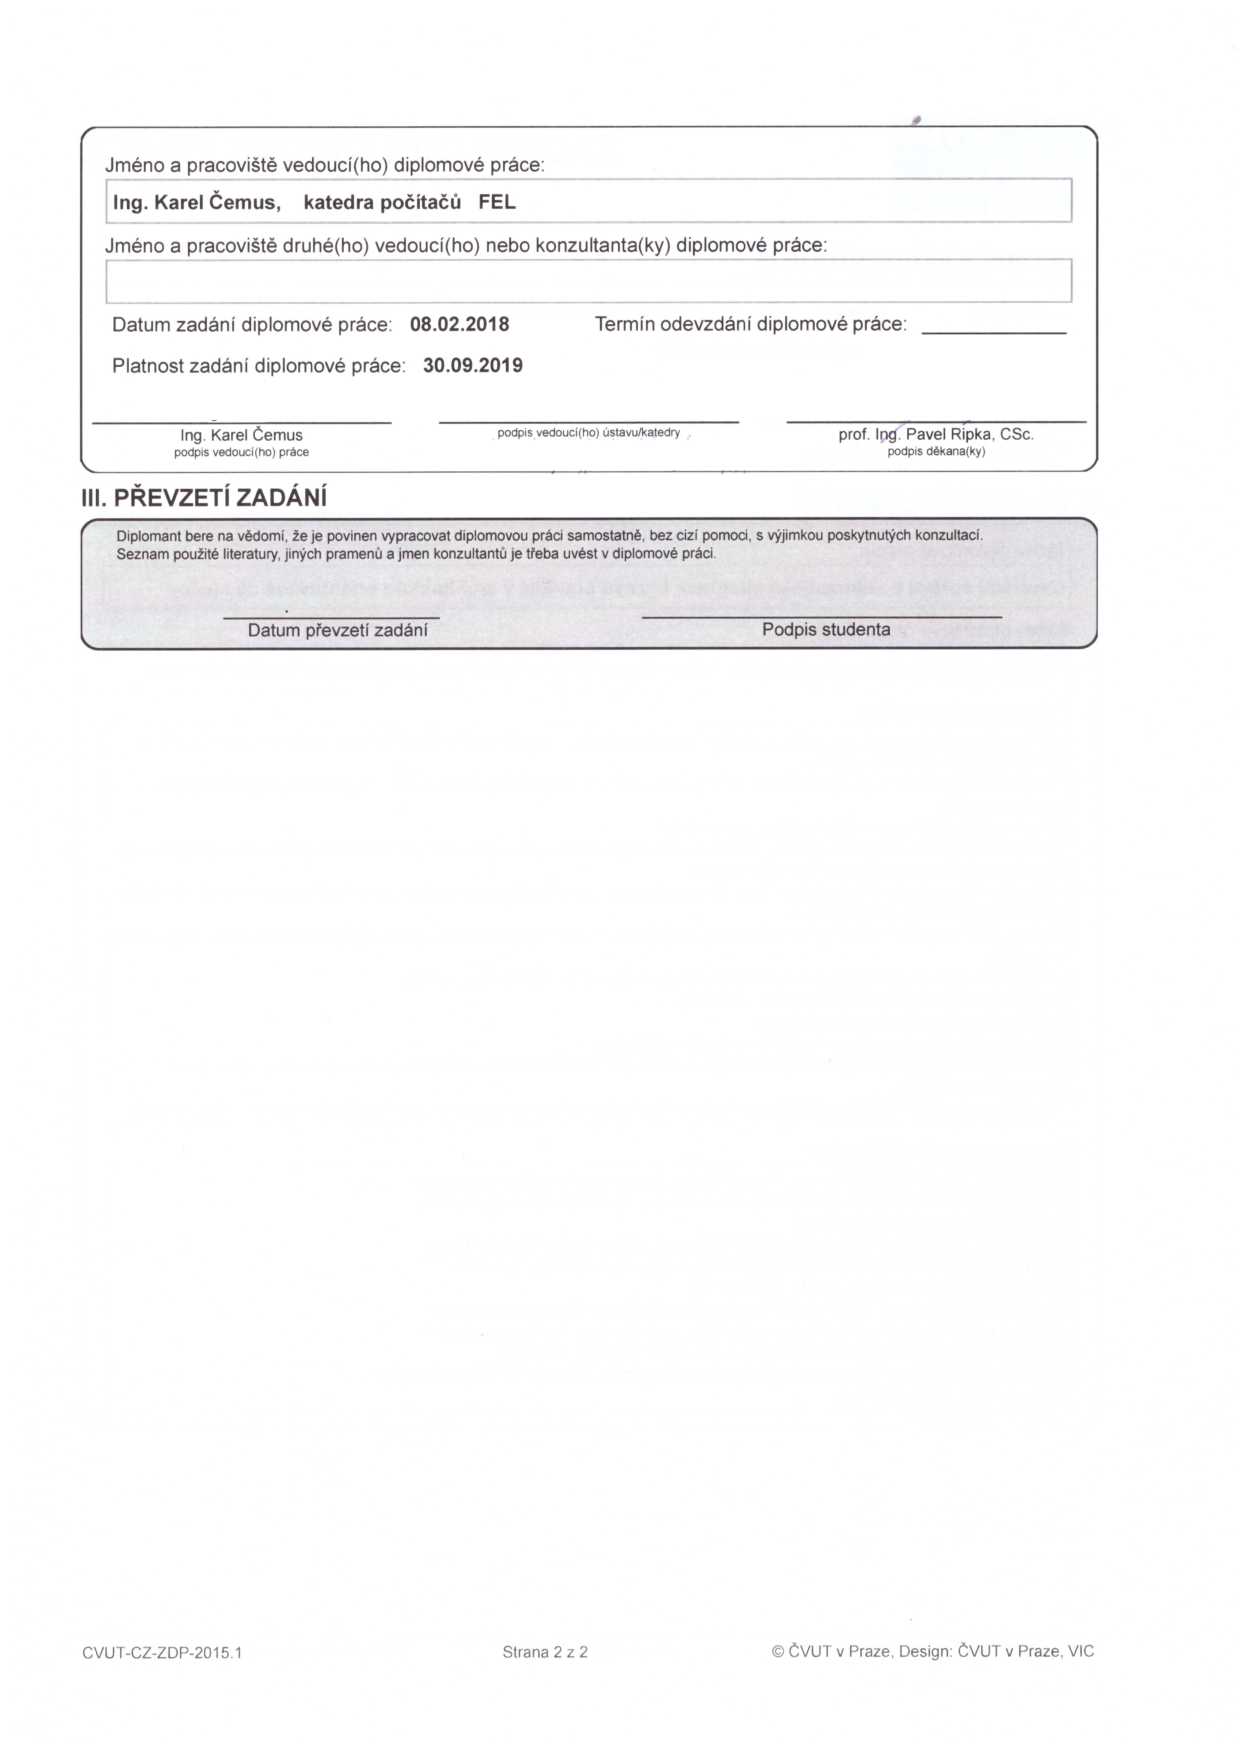
\includepdf[pages=1,pagecommand={}]{figures/zadani-back.pdf}
\newpage
}

%%%%%%%%%%%%%%%%%%%%%%%%%%
% Titulni stranka / Title page
\coverpagestarts

%%%%%%%%%%%%%%%%%%%%%%%%%%%
% Poděkovani / Acknowledgements

\acknowledgements
\noindent
Chtěl bych poděkovat Ing. Karlovi Čemusovi za jeho trpělivost, podporu a
cenné rady nejen při vedení této práce, ale po celou dobu mého studia.
Děkuji své rodině, přítelkyni a přátelům za zázemí a podporu, kterou
mi po dobu studia poskytovali a bez které bych ho nemohl dokončit.
Děkuji také svým kolegům ve škole i v zaměstnání, kteří mě motivovali k
dosažení vynikajících výsledků v průběhu magisterského studia.


%%%%%%%%%%%%%%%%%%%%%%%%%%%
% Prohlášení / Declaration

\declaration{V~Praze dne 23.\,5.\,2018}
%\declaration{In Kořenovice nad Bečvárkou on May 15, 2008}


%%%%%%%%%%%%%%%%%%%%%%%%%%%%
% Abstrakt / Abstract

\abstractpage

%Translation of Czech abstract into English.
\noindent{Service-oriented architecture decomposes information systems into small
standalone services lowering their complexity through loose coupling
and component reuse. Business rules often cross-cut multiple services and
must be addressed consistently. Current approaches reach their limits when it
comes to the business rules. They tend to require manual information restatement and
code duplication, which raises development and maintenance costs and efforts.}

\vspace{\baselineskip}

\noindent{This thesis analyses the problem of business rules in service-oriented
architecture and proposes a novel approach that uses aspect-oriented
programming to enable central administration and automatic integration
of business rules in such systems. Moreover, the thesis provides a proof of concept
showing reduction of manual duplication of business rules within an example system
utilizing the proposed approach.}

\vspace{\baselineskip}

\noindent{\textbf{Keywords:} Service-oriented architecture, enterprise information systems, business rules, aspect-oriented programming, separation of concerns}

% Prace v cestine musi krome abstraktu v anglictine obsahovat i
% abstrakt v cestine.
\vglue25mm

\noindent{\LARGE \textbf{Abstrakt}}
\vspace{\baselineskip}

\noindent{Architektura orientovaná na služby člení funkcionalitu komplexních
informačních systémů do samostatných služeb a díky tomu usnadňuje oddělení
zodpovědností a zvyšuje znovupoužitelnost jednotlivých komponent.
Byznysová pravidla ale často zasahují do více služeb najednou a vyžadují
konzistentní vykonávání. To při použití současných přístupů vede k manuální
duplikaci pravidel, která zvyšuje náklady na vývoj a údržbu systémů.}

\vspace{\baselineskip}

\noindent{Tato práce analyzuje problematiku byznysových pravidel v architektuře orientované
na služby a navrhuje alternativní způsob, jakým lze s využitím aspektově orientovaného
programování usnadnit práci vývojářů a administrátorů pomocí centrální správy a
automatické integrace těchto pravidel. Součástí práce je implementace navrženého přístupu na
ukázkovém příkladu, který demonstruje snížení manuální duplikace byznysových pravidel.}

\vspace{\baselineskip}

\noindent{\textbf{Klíčová slova:} Architektura orientovaná na služby, podnikové informační systémy, byznysová pravidla, aspektově orientované programování}

%\noindent
%Abstrakt práce by měl velmi stručně vystihovat její obsah. Tedy čím se práce zabývá a co je jejím výsledkem/přínosem.

%\noindent
%Očekávají se cca 1 -- 2 odstavce, maximálně půl stránky.

%%%%%%%%%%%%%%%%%%%%%%%%%%
% obsahy a seznamy
\renewcommand{\lstlistlistingname}{Seznam zdrojových kódů}
\renewcommand{\lstlistingname}{Zdrojový kód}

\setcounter{tocdepth}{1}
\begingroup
\hypersetup{linkcolor=black}
\tableofcontents

% pokud v práci nejsou obrázky nebo tabulky - odstraňte jejich seznam
\listoffigures            % Obsah / Table of Contents
\listoftables            % Seznam tabulek / List of Tables

\lstset{
basicstyle=\fontsize{10}{12}\selectfont\ttfamily
}
\lstlistoflistings
\endgroup

%%%%%%%%%%%%%%%%%%%%%%%%%%
% začátek textu
\mainbodystarts

%!TEX ROOT=../diploma-thesis.tex

\chapter{Úvod}\label{ch:uvod}

%\goal{Informační systémy a jejich důležitost}
Informační systémy se ve 21. století staly neodmyslitelnou součástí našich každodenních životů.
Do styku s nimi přicházíme jak při výkonu našich povolání, tak ve volném čase. Usnadňují
řadu aspektů našich činností. Jejich využití sahá do mnoha sektorů, od vzdělání a vědy,
kde mimo jiné významně usnadňují přístup ke studijním materiálům, přes zdravotnictví,
kde pomáhají zvyšovat efektivitu a úroveň péče o pacienty~\cite{fichman2011editorial}, až po
sociální sítě, kde umožňují lidem globálně komunikovat a sdílet své myšlenky, pocity a zážitky.
Jedním z úkolů výzkumu v oblasti softwarového inženýrství je zjednodušení a zefektivnění procesu
vývoje informačních systémů. Díky tomu budou tyto systémy moci splňovat stále rostoucí množství požadavků.

%\goal{SOA}
Náročnost vývoje některých informačních systémů překračuje možnosti jednotlivců, ale
i celých týmů či skupin. Tyto systémy často využívají větší počet různorodých technologií kvůli
širokému spektru funkcionality, kterou nabízejí. Jedním z přístupů, který tyto problémy řeší,
je použití architektury orientované na služby. Ta se zaměřuje na sestavení systému z menších, vzájemně
nezávislých celků, tzv. služeb. Každá služba pak zastřešuje pouze část funkcionality systému.
Tím je umožněno využívat teoreticky neomezené množství technologií a rozdělit práci na systému mezi více nezávislých
vývojářských týmu.

%\goal{Byznysová pravidla}
Tato architektura bohužel nepřináší odpověď na všechny problémy, které je potřeba v informačních
systémech řešit. Jak je popsáno v následujících kapitolách, jedním z těchto problémů jsou tzv. byznysová
pravidla. Ta slouží k zajištění správné funkcionality systému a konzistenci uložených dat.
Některá tato pravidla zasahují do celého systému, tedy i do více služeb.
To při použití konvenčního přístupu přináší nutnost manuální duplikace zdrojového
kódu a tím jsou zvýšeny náklady na vývoj systému a riziko lidské chyby.

%\goal{Motivace a cíle}
Cílem této práce je prozkoumat myšlenku inovativního přístupu k centrální správě a automatické
integraci byznysových pravidel v systémech využívajících architekturu orientovanou na služby
a navrhnout framework, který by umožnil tento přístup uplatnit v praxi.
Tento koncept by měl díky využití aspektově orientovaného programování usnadnit práci vývojářů
a doménových expertů. Díky tomu by mohl přinést snížení nákladů na vývoj a údržbu informačních systémů
a tím zvýšit jejich kvalitu a snížit náklady na jejich vývoj.

%\goal{Popis struktury DP a obsah kapitol}
Kapitola~\ref{ch:analyza} se věnuje detailn\'{\i} anal\'yze problematiky bynysov\'ych pravidel a
architektury orientované na služby, včetně jej\'{\i}ho historického v\'yvoje až po nejnovějš\'{\i} trendy,
a v závěru identifikuje požadavky kladené na framework pro centráln\'{\i} správu a
automatickou integraci byznysov\'ych pravidel v této architektuře. Kapitola~\ref{ch:reserse}
se zab\'yvá rešerš\'{\i} stávaj\'{\i}c\'{\i}ch pr\'{\i}stupu k v\'yvoji informacn\'{\i}ch systému a speciálně se zaměřuje
na koncepty aspektově orientovaného programován\'{\i} a modern\'{\i}ho aspekty ř\'{\i}zeného př\'{\i}stupu k návrhu
systémů. Dále se kapitola věnuje průzkumu existuj\'{\i}c\'{\i}ch nástrojů pro správu byznysov\'ych pravidel a existujícím
síťovým architekturám, které budou sloužit pro distribuci byznysových pravidel mezi službami.
Kapitola~\ref{ch:navrh} formalizuje prostřed\'{\i} architektury orientované na služby do terminologie
aspektově orientovaného programován\'{\i} a na základě této formalizace navrhuje koncept frameworku,
kter\'y realizuje centráln\'{\i} správu a automatickou integraci byznysov\'ych pravidel.
V kapitole~\ref{ch:implementace} je detailně probrána implementace knihoven pro navržen\'y framework
pro platformy jazyků Java a Python a frameworku Node.js. Následuj\'{\i}c\'{\i} kapitola~\ref{ch:verifikace}
popisuje, jak\'ym způsobem byly tyto knihovny otestovány a jak byla prokázána jejich funkčnost. Zároveň
je zde popsána validace a vyhodnocen\'{\i} konceptu frameworku jeho nasazen\'{\i}m při v\'yvoji
jednoduchého ukázkového e-commerce systému. V posledn\'{\i} kapitole~\ref{ch:zaver} je shrnuto, jak\'ych
c\'{\i}lů bylo v práci dosáhnuto a jak\'ym dalš\'{\i}m směrem se může v\'yzkum v této oblasti ub\'{\i}rat.

%!TEX ROOT=../diploma-thesis.tex

\chapter{Anal\'yza}\label{ch:analyza}

Tato kapitola analyzuje problematiku byznysov\'ych pravidel v informačn\'{\i}ch systémech.
Dále detailně popisuje architekturu orientovanou na služby, včetně jej\'{\i}ho historického
v\'yvoje a modern\'{\i}ho trendu v podobě microservices. Na základě toho kapitola popisuje nedostatky
současn\'ych př\'{\i}stupů při řešen\'{\i} průřezov\'ych problémů v těchto architekturách, s důrazem na byznysová pravidla.
V závěru kapitoly jsou identifikovány požadavky, které by měl splňovat framework,
jež bude v\'ystupem této diplomové práce.

\section{Byznysová pravidla}

Informačn\'{\i} systémy (\gls{IS}) maj\'{\i} za úkol ulehčit, automatizovat či poskytovat podporu pro
byznysové procesy společnost\'{\i}, které je využ\'{\i}vaj\'{\i}. Tyto procesy jsou tedy stěžejn\'{\i}m
prvkem \gls{IS}. Systém má také za úkol uchovávat a spravovat data společnosti
a měl by zaručit, že nedojde k jejich poškozen\'{\i} či narušen\'{\i} jejich integrity.
Byznysové procesy, potažmo byznysové operace, proto musej\'{\i}
podléhat jasně definovan\'ym byznysov\'ym pravidlům, která zajišťuj\'{\i} konzistenci dat informačn\'{\i}ho
systému a také zabraňuj\'{\i} nepovolen\'ym operac\'{\i}m~\cite{cemus2015automated}.

Byznysová pravidla děl\'{\i}me do tř\'{\i} skupin~\cite{cemus2014aspect}:
\begin{description}
    \item [Bezkontextová pravidla] jsou validačn\'{\i} pravidla, která musej\'{\i} b\'yt obecně platná
    v každé operaci, jinak by mohlo doj\'{\i}t k porušen\'{\i} integrity dat systému. Př\'{\i}kladem může
    b\'yt pravidlo \uv{\textit{Adresa uživatele je platnou e-mailovou adresou}}.
    \item [Kontextová pravidla] jsou pravidla, která musej\'{\i} b\'yt zohledněna v daném kontextu
    byznysové operace, např\'{\i}klad \uv{\textit{Při přidán\'{\i} produktu do koš\'{\i}ku nesm\'{\i} součet položek
    v koš\'{\i}ku přesahovat částku milion korun}}
    \item [Průřezová pravidla] jsou parametrizována stavem systému nebo uživatelského účtu a maj\'{\i}
    dopad na velkou část byznysov\'ych operac\'{\i}. Uvažme pravidlo \uv{\textit{V systému nesm\'{\i} prob\'{\i}hat
    žádné změny po dobu účetn\'{\i} uzávěrky}}.
\end{description}

Dále také rozlišujeme dva typy byznysov\'ych pravidel, a těmi jsou \textit{preconditions}
a \textit{post-conditions}~\cite{cemus2015automated}.

\subsection{Precondition}

Aby mohla b\'yt byznysová operace vykonána, musej\'{\i}
b\'yt splněny předem definované podm\'{\i}nky, neboli předpoklady,
které naz\'yváme \textit{preconditions}. Pokud alespoň jedna z podm\'{\i}nek
nen\'{\i} splněna, byznysová operace nemůže proběhnout.

Pro lepš\'{\i} ilustraci uveďme př\'{\i}klad: aby mohla b\'yt provedena
registrace uživatele s danou emailovou adresu, mus\'{\i} b\'yt splněna
podm\'{\i}nka, že uživatel vyplnil svoj\'{\i} emailovou adresu, a zároveň
dosud v systému neexistuje žádn\'y uživatel se stejnou emailovou adresou.

\subsection{Post-condition}

Na byznysovou operaci mohou b\'yt kladeny požadavky, které
musej\'{\i} b\'yt splněny po jej\'{\i}m úspěšném vykonán\'{\i}. Př\'{\i}kladem
může b\'yt anonymizace uživatelů při vytvářen\'{\i} statistického
reportu e-commerce společnosti – po vygenerován\'{\i} reportu
post-condition zajist\'{\i}, že z něj budou smazány veškeré citlivé údaje.
Dalš\'{\i}m př\'{\i}padem může b\'yt filtrován\'{\i} v\'ystupu byznysové operace.
Např\'{\i}klad při v\'ypisu objednávek pro zákazn\'{\i}ka se chceme ujistit, že
všechny vypsané objednávky patř\'{\i} danému zákazn\'{\i}kovi.

\subsection{Reprezentace byznysového pravidla}

Existuje několik možnost\'{\i}, jak zachytit a reprezentovat byznysová pravidla~\cite{cemus2015automated}.
Nejběžnějš\'{\i} a nejpouž\'{\i}vanějš\'{\i} metodou je jejich zachycen\'{\i} v programovac\'{\i}m
jazyce. Tato metoda je snadná, protože programátor může použ\'{\i}t stejn\'y jazyk
pro popis pravidel stejně jako pro popis celého systému. Bohužel, tato metoda
nám nedává př\'{\i}liš možnost\'{\i} jak provést inspekci a extrakci pravidel.
Dalš\'{\i}, pokročilejš\'{\i} metodou, je zápis pravidel pomoc\'{\i} meta-instrukc\'{\i}, např\'{\i}klad anotac\'{\i},
nebo tzv.\textit{Expression Language} (\gls{EL}). Tato metoda poskytuje dobrou možnost inspekce,
ale zpravidla nen\'{\i} typově bezpečná a může snáze způsobovat chyby v programu.
Posledn\'{\i}, nejpokročilejš\'{\i} metodou, je zápis pomoc\'{\i} doménově specifick\'ych jazyků.
Ty jsou snadno srozumitelné nejen pro programátory, ale i pro doménové experty.
Nevyžaduj\'{\i} inspekci a mohou b\'yt typově bezpečné. Mezi jejich nev\'yhody ale patř\'{\i} vysoká
počátečn\'{\i} investice v podobě návrhu takového jazyka a nutnost jeho kompilace nebo
interpretace.

\subsection{Byznysov\'y kontext}

Informačn\'{\i} systém zpravidla implementuje v\'{\i}ce byznysov\'ych procesů, které se vážou
na jeden či v\'{\i}ce uživatelsk\'ych scénářů. Uživatelsk\'y scénář se pak děl\'{\i} na jednotlivé
kroky, např\'{\i}klad zaslán\'{\i} potvrzovac\'{\i}ho e-mailu k objednávce, či uložen\'{\i} objednávky
do databáze. Tyto kroky naz\'yváme \textit{byznysové operace} – tedy operace, které maj\'{\i}
byznysovou hodnotu. Ke každé byznysové operaci př\'{\i}sluš\'{\i} množina byznysov\'ych pravidel,
konkrétně preconditions a post-conditions.

Při běhu informačn\'{\i}ho systému je v paměti držen tzv. \textit{exekučn\'{\i} kontext} (z anglického \textit{execution context}),
kter\'y se skládá z několika d\'{\i}lč\'{\i}ch kontextů~\cite{cemus2017separation}. Prvn\'{\i}m
je \textit{aplikačn\'{\i} kontext} (z anglického \textit{application context}), ve kterém je uložen stav globálnc\'{\i}h proměnn\'ych systému,
jako např. nastaven\'{\i} produkčn\'{\i}ho režimu, nebo př\'{\i}znak o tom, zda právě prob\'{\i}há obchodn\'{\i}
uzávěrka. Dalš\'{\i}m je \textit{uživatelsk\'y kontext}, kter\'y obsahuje informace o aktuálně
přihlášeném uživateli. \textit{Kontext požadavku} (z anglického \textit{Request context}) obsahuje
informace o aktuáln\'{\i}m požadavku, jako IP adresa uživatele či jeho geolokace,
a vztahuje se zejména k webov\'ym službám. Posledn\'{\i}m je \textit{byznysov\'y kontext}. Ten
chápeme jako množinu preconditions a post-conditions s byznysovou hodnotou, která se
váže na konkrétn\'{\i} byzynsovou operaci~\cite{cemus2015automated}.
Abychom mohli efektivně definovat co nejširš\'{\i} škálu byzynsov\'ych pravidel,
musej\'{\i} při jejich vyhodnocován\'{\i} b\'yt dostupné proměnné exekučn\'{\i}ho kontextu,

\section{Architektura orientovaná na služby}\label{sec:soa}

\goal{Úvod do SOA, proč je potřeba}
V posledn\'{\i}ch dekádách můžeme sledovat trend nárůstu komplexity
modern\'{\i}ch informačn\'{\i}ch systémů, kter\'y je způsoben stále náročnějš\'{\i}mi
požadavky na jejich funkcionalitu, v\'ykon a spolehlivost. To nut\'{\i}
v\'yvojáře těchto systémů přizpůsobovat architekturu systému tak,
aby uměla splnit všechny očekávané funkčn\'{\i} i nefunkčn\'{\i} požadavky,
zejména pak škálovatelnost systému a jeho schopnost zvládat vysok\'y
objem dat a uživatelů. \textit{Architektura orientovaná na služby} (\gls{SOA}) je
důsledkem této evoluce. Na rozd\'{\i}l od dř\'{\i}vě běžné a dnes
stále použ\'{\i}vané \textit{monolitické architektury},
\gls{SOA} podle známého pravidla \uv{rozděl a panuj}
děl\'{\i} systém na samostatné celky, zvané \textit{služby}, které jsou
zodpovědné za d\'{\i}lč\'{\i} část požadované funkcionality.

\goal{Proč tu vlastně p\'{\i}šu o nějaké historii}
Historicky byl term\'{\i}n \gls{SOA} vykládán různ\'ymi způsoby a v\'yvojáři si
pod n\'{\i}m představovali několik rozd\'{\i}ln\'ych, nekompatibiln\'{\i}ch
konceptů~\cite{fowler2005serviceorientedambiguity}.
Zejména pak absence kvalitn\'{\i}ch definic toho, co vlastně
služba je, vedla k vzájemnému nedorozuměn\'{\i}, zmaten\'{\i} a v posledn\'{\i}
době i ke snahám o opuštěn\'{\i} tohoto konceptu~\cite{cerny2017disambiguation}.
Abychom lépe prozuměli tomu, co vlastně \gls{SOA} je, pop\'{\i}šeme si jej\'{\i} historick\'y
v\'yvoj a shrneme v\'yhody a nev\'yhody jednotliv\'ych př\'{\i}stupů.

\subsection{Common Object Request Broker Architecture}\label{sec:corba}

Prvn\'{\i}m historick\'ym předchůdcem architektury orientované na služby
byla tzv. \textit{Common Object Request Broker Architecture}
(\gls{CORBA})~\cite{siegel2000corba}, která vzikala v osmdesát\'ych a devadesát\'ych letech
dvacátého stolet\'{\i}. Ta umožňuje komunikaci mezi aplikacemi implementovan\'ymi v
různ\'ych technologi\'{\i}ch a běž\'{\i}c\'{\i}mi na vlastn\'{\i}ch stroj\'{\i}ch s rozd\'{\i}ln\'ymi
operačn\'{\i}mi systémy. Základn\'{\i}m stavebn\'{\i}m kamenem této architektury
je \textit{Object Request Broker} (\gls{ORB}), kter\'y emuluje objekty,
na kter\'ych může klient volat jejich metody. Při zavolán\'{\i} metody
na objektu, kter\'y se fyzicky nacház\'{\i} v aplikaci na vzdáleném stroji,
zprostředkovává \gls{ORB} veškerou komunikaci a svému uživateli poskytuje
jeho kompletn\'{\i} rozhran\'{\i}. Uživatel tedy de facto nerozezná, kdy volá
metodu na objektu, kter\'y je lokálně dostupn\'y,
a kdy volá metodu, kterou obsouž\'{\i} vzdálená služba. To je ale zároveň
hlavn\'{\i} nev\'yhodou této architektury, protože komunikace se vzdálen\'ym
objektem s sebou nese celou řadu problémů, např\'{\i}klad mnohem vyšš\'{\i} latenci
při komunikaci nebo v\'yjimečné stavy, které je potřeba ošetřit. Ve chv\'{\i}li,
kdy klient nen\'{\i} schopen rozeznat mezi metodou volanou lokálně či vzdáleně,
se těžko přizpůsobuje těmto okolnostem, což vnáš\'{\i} do kódu zbytečnou
komplexitu a zhoršuje jeho kvalitu kvůli obt\'{\i}žnějš\'{\i} optimalizaci.

\subsection{Web Services}

Nedostatky architektury \gls{CORBA} vedly k volbě jednodušš\'{\i}ho
formátu pro popis komunikace služeb, spolehlivějš\'{\i}ho a méně
komplikovaného kanálu pro komunikaci a celkové redukci
objemu komunikovan\'ych dat. Preferovanou cestou komunikace
se na přelomu tis\'{\i}cilet\'{\i} stal protokol \gls{HTTP}, zat\'{\i}mco preferovan\'ym formátem
pro serializaci přenášen\'ych dat se stal jazyk \gls{XML}.
Postupně se upustilo od volán\'{\i} metod na vzdálen\'ych objektech a přijal
se koncept explicitn\'{\i}ho pos\'{\i}lán\'{\i} zpráv mezi službami.
Pro popis schématu zpráv vznikl formát \textit{Simple Object Access
Protocol} (\gls{SOAP})~\cite{box2000simple}, kter\'y v kombinaci s
\textit{Web Service Description Language} (\gls{WSDL})~\cite{christensen2001web}
umožňuje kompletn\'{\i} definici rozhran\'{\i} pro komunikaci mezi službami.
V průběhu dalš\'{\i}ch let vznikla také velmi populárn\'{\i} architektura
\textit{Representational State Transfer} (\gls{REST})~\cite{fielding2000rest},
která pro popis webov\'ych služeb využ\'{\i}vá čistě protokol \gls{HTTP} a jeho slovesa.
To službám přináš\'{\i} společn\'y slovn\'{\i}k a umožňuje snažš\'{\i} dokumentaci
a rychlejš\'{\i} orientaci v\'yvojářů, kteř\'{\i} takovou službu implementuj\'{\i} či konzumuj\'{\i}.
Kvůli těžkopádnosti \gls{XML} se pro služby implementuj\'{\i}c\'{\i} \gls{REST} architekturu stal
preferovan\'ym formátem přenosu \textit{JavaScript Object Notation} (\gls{JSON}).
Nejnovějš\'{\i}m formátem pro popis služeb, čerpaj\'{\i}c\'{\i} z nedostatků architektury \gls{REST}, je
\textit{GraphQL}, se kter\'ym v roce 2015 přišla společnost Google.

\subsection{Message Queue}

\begin{figure}
    \centering
    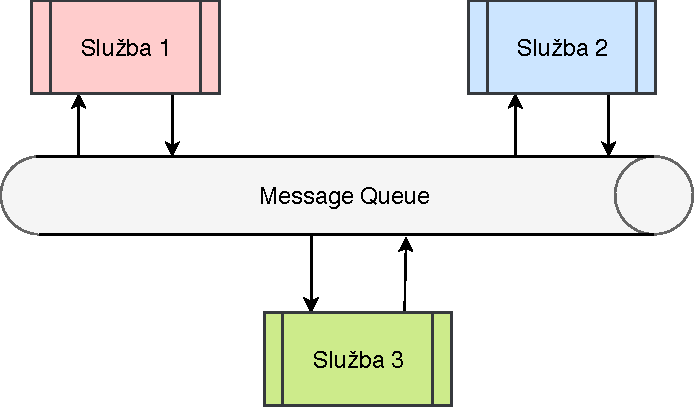
\includegraphics[keepaspectratio=true, width=0.5\linewidth]{figures/message-queue.pdf}
    \caption{Komunikace služeb pomoc\'{\i} Message Queue}
    \label{fig:message-queue}
\end{figure}

Dalš\'{\i}m z konceptů, kter\'y v rámci \gls{SOA} vznikl, je tzv. \textit{Message Queue} (\gls{MQ}).
Základn\'{\i} myšlenkou \gls{MQ}, znázorněnou na obrázku~\ref{fig:message-queue},
je asynchronn\'{\i} komunikace služeb pomoc\'{\i} zpráv nezávisl\'ych
na platformě. Komunikaci zprostředkovává fronta, která přij\'{\i}má a rozes\'{\i}lá
zprávy mezi službami. To přináš\'{\i} vyšš\'{\i} škálovatelnost a menš\'{\i} provázanost
mezi službami. Všechny služby ale mus\'{\i} použ\'{\i}vat jednotn\'y formát zpráv.

\gls{MQ} přináš\'{\i} dva způsoby, kter\'ymi mohou služby komunikovat. Prvn\'{\i}m je
\textit{Request/Reply}, připom\'{\i}naj\'{\i}c\'{\i} konverzaci dvou lid\'{\i}. Jedna
služba zašle zprávu obsahuj\'{\i}c\'{\i} identifikátor konverzace. Druhá služba
na obdrženou zprávu zašle odpověď a pomoc\'{\i} identifikátoru označ\'{\i},
ke které otázce odpověď patř\'{\i}. Druh\'ym způsobem je \textit{publish-subscribe},
kdy existuje v\'{\i}ce front s různ\'ymi tématy (\textit{topics}) a služby mohou
do těchto front přisp\'{\i}vat relevantn\'{\i}mi zprávami nebo je konzumovat jako odběratelé.

\subsection{Enterprise Service Bus}

Ačkoliv zm\'{\i}něné modely usnadňuj\'{\i} komunikaci služeb a zvyšuj\'{\i} jejich
spolehlivost, integrace služeb může b\'yt obt\'{\i}žná, pokud služby použ\'{\i}vaj\'{\i} navzájem různé
komunikačn\'{\i} protokoly a formáty. Již v devadesát\'ych letech minulého stolet\'{\i}
byl představen koncept \textit{Enterprise Service
Bus} (\gls{ESB})~\cite{chappell2004enterprise},
znázorněn\'y na obrázku~\ref{fig:enterprise-service-bus},
kter\'y má za úkol propojit heterogenn\'{\i} služby a zajistit mezi nimi
komunikačn\'{\i} kanály. T\'{\i}m na sebe \gls{ESB} přeb\'{\i}rá zodpovědnost za překlad
jednotliv\'ych zpráv a centralizuje veškerou komunikaci v systému.

\gls{ESB} se zároveň stav\'{\i} do role experta na lokalizaci jednotliv\'ych služeb.
Službě tak pro komunikaci s okoln\'{\i}m světem stač\'{\i} znát adresu \gls{ESB}, kterému
zašle zprávu, a ten ji sám doruč\'{\i} na m\'{\i}sto určen\'{\i}. Tento model ale
znamená, že \gls{ESB} je velmi komplexn\'{\i} komponentou. V\'ypadek \gls{ESB} nav\'{\i}c
v způsob\'{\i} zastaven\'{\i} funkce celého systému a \gls{ESB} se tak stává
tzv. \textit{single point of failure}, což v praxi snižuje škálovatelnost systému.
V př\'{\i}padě vlastn\'{\i}ho n\'{\i}zkého v\'ykonu se \gls{ESB} může snadno stát úzk\'ym hrdlem.
Tyto problémy mohou b\'yt částečně vyřešeny tzv. \textit{federovan\'ym designem},
kdy je systém rozdělen na byznysově př\'{\i}buzné části, z nichž každá má
svůj \gls{ESB}.

\begin{figure}
    \centering
    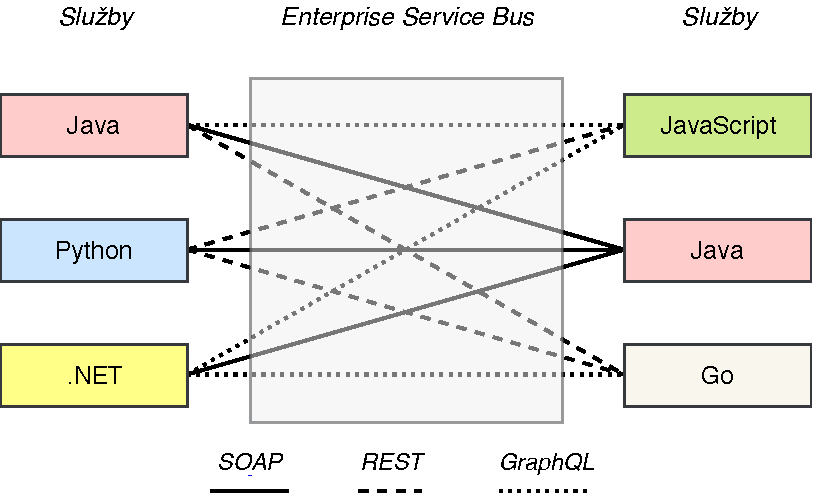
\includegraphics[keepaspectratio=true, width=0.7\linewidth]{figures/enterprise-service-bus.pdf}
    \caption{Komunikace služeb skrz Enterprise Service Bus}
    \label{fig:enterprise-service-bus}
\end{figure}

\subsection{Microservices}

\goal{Microservices a budoucnost SOA}
Nov\'ym trendem posledn\'{\i}ch let jsou takzvané \textit{Microservices}.
Přináš\'{\i} několik zajmav\'ych konceptů, které specializuj\'{\i} a konkretizuj\'{\i}
principy \gls{SOA}. Microservices se tedy daj\'{\i} chápat jako podmnožina
\gls{SOA}. Základn\'{\i} myšlenkou je v\'yvoj informačn\'{\i}ho systému jako množiny
mal\'ych oddělen\'ych služeb, které jsou spouštěny v samostatn\'ych procesech
a komunikuj\'{\i} spolu pomoc\'{\i} jednoduch\'ych protokolů~\cite{lewis2014microservices}.

\goal{Stavba služeb kolem byznysov\'ych schopnost\'{\i}}
Důležitou myšlenkou microservices je organizace služeb kolem
byznysov\'ych schopnost\'{\i} systému. Nam\'{\i}sto horizontáln\'{\i}ho dělen\'{\i} systému
podle jeho vrstev\footnote{
Zde předpokládáme klasickou tř\'{\i}vrstvou architekturu~\cite{fowler2002patterns},
rozděluj\'{\i}c\'{\i} systém na \textit{datovou vrstvu}, \textit{aplikačn\'{\i} vrstvu}
a \textit{prezentačn\'{\i} vrstvu}. Tyto vrstvy maj\'{\i} oddělené zodpovědnosti a komunikuj\'{\i}
spolu pomoc\'{\i} jasně definovan\'ych společn\'ych rozhran\'{\i}.
} navrhuje rozdělit systém vertikálně podle jeho byznysov\'ych schopnost\'{\i}.
Na obrázku~\ref{fig:monolith-vs-microservices} je toto rozdělen\'{\i} demonstrováno.
Př\'{\i}kladem může b\'yt dělen\'{\i} e-commerce systému na jednu službu obsahuj\'{\i}c\'{\i} byznysovou
logiku pro registraci a správu uživatelů, druhou službu obsahuj\'{\i}c\'{\i} byznysovou logiku
pro práci s produkty a třet\'{\i} službu obsahuj\'{\i}c\'{\i} byznysovou logiku pro práci
s objednávkami.

\begin{figure}
    \centering
    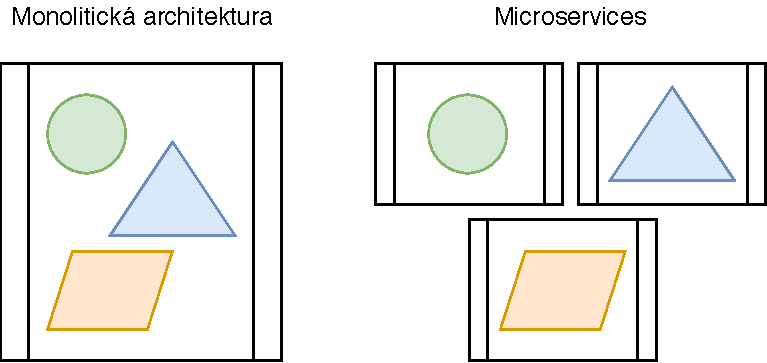
\includegraphics[keepaspectratio=true, width=0.5\linewidth]{figures/monolith-vs-microservices.pdf}
    \caption{Porovnán\'{\i} struktury monolitické architektury a microservices}
    \label{fig:monolith-vs-microservices}
\end{figure}

\goal{Myšlenka nahraditelnosti komponenty}
Koncept microservices přem\'yšl\'{\i} o službě jako o samostatné komponentě,
kterou lze individuálně vyměnit či vylepšit, bez nutnosti zásahu do
ostatn\'{\i}ch služeb~\cite{lewis2014microservices}. Monolitická architektura
vyžaduje i při malé změně jedné části cel\'y systém znovu zkompilovat, sestavit
a nasadit. Malé služby slouž\'{\i}c\'{\i} ideálně jedinému byznysovému účelu lze naopak
při změně byznysov\'ych požadavků snadno nahradit samostatně bez zásahu do zbytku
systému. T\'{\i}m se usnadňuje cyklus nasazen\'{\i} a spuštěn\'{\i} nové verze služby.

\goal{Myšlenka smart endpoints, dumb pipes}
Microservices také přinášej\'{\i} koncept \uv{smart endpoint, dumb pipes},
kter\'y opoušt\'{\i} koncept \gls{ESB} ve prospěch přesunut\'{\i} veškeré byznys logiky
na stranu služeb. T\'{\i}m se zvyšuje zapouzdřenost služeb a snižuje se
jejich vzájemné provázán\'{\i}. Nutno podotknout, že microservices často
využ\'{\i}vaj\'{\i} ke své funkci Message Queues.

\paragraph{Škálovatelnost}
Dalš\'{\i} nespornou v\'yhodou microservices je vysoká škálovatelnost systému. Pokud je na
některou ze služeb kladen vyšš\'{\i} nárok na v\'ykon než na ostatn\'{\i}, maj\'{\i}
v\'yvojáři možnost konkrétn\'{\i} službu horizontálně škálovat aniž by
museli škálovat kompletně cel\'y systém, na rozd\'{\i}l od monolitické architektury.
Srovnán\'{\i} př\'{\i}stupů je znázorněno na obrázku~\ref{fig:microservices-deployment}.
D\'{\i}ky této vlastnosti je možné sn\'{\i}žit nároky na systémové zdroje při zachován\'{\i}
stejného v\'ykonu.

\paragraph{Využit\'{\i} rozlišn\'ych technologi\'{\i}}
Monolitické aplikace jsou často implementovány v jednom programovac\'{\i}m jazyce
a využ\'{\i}vaj\'{\i} omezenou množinu technologi\'{\i}. Ne pro každ\'y úkol je ale vhodn\'y
jeden programovac\'{\i} jazyk a s rostouc\'{\i} velikost\'{\i} informačn\'{\i}ho systému často roste
i rozmanitost jeho funkcionality. Rozdělen\'{\i}m systému na v\'{\i}ce služeb, které
komunikuj\'{\i} protokolem nezávisl\'ym na platformě, je v\'yvojářům umožněno využ\'{\i}t
širš\'{\i} spektrum technologi\'{\i} a implementovat požadovanou funkcionalitu
efektivněji.

\begin{figure}
    \centering
    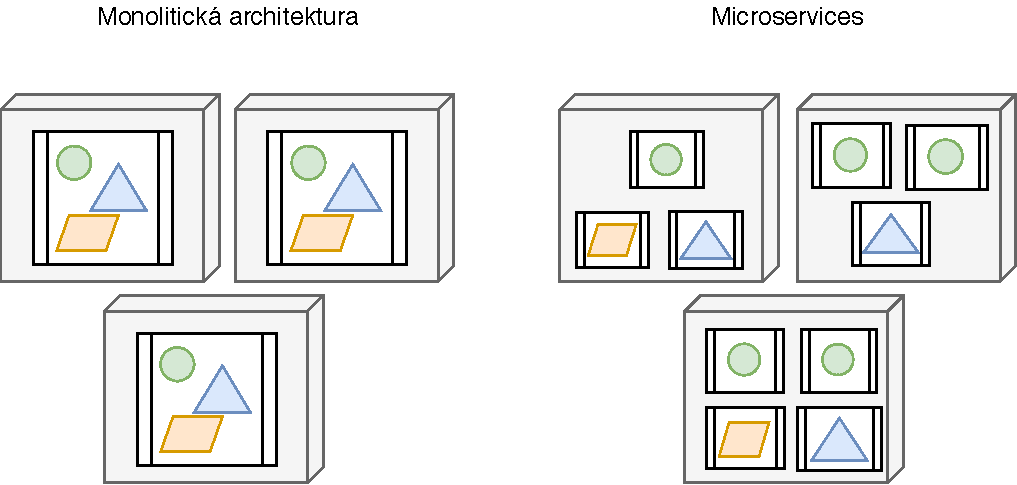
\includegraphics[keepaspectratio=true, width=0.8\linewidth]{figures/microservices-deployment.pdf}
    \caption{Porovnán\'{\i} nasazen\'{\i} monolitické architektury a microservices}
    \label{fig:microservices-deployment}
\end{figure}

\paragraph{Decentralizace úložiště}
Dalš\'{\i}m z principů, které microservices přináš\'{\i}, je oddělen\'{\i} a decentralizace
databázového úložiště. Každá služba, či cluster instanc\'{\i} jedné služby, zapisuj\'{\i}
a čtou data ze své oddělené databáze. Pokud potřebujou nač\'{\i}st data jiné služby,
musej\'{\i} k tomu využ\'{\i}t jej\'{\i} \gls{API}. T\'{\i}m se ještě v\'yrazněji odděluje zodpovědnost služeb.
Typickou praktikou v rámci \gls{SOA} je naopak sd\'{\i}len\'{\i} jedné databáze mezi v\'{\i}ce službami,
což je často dáno komerčn\'{\i}m modelem extern\'{\i}ho dodatavele databáze. Jediná databáze
má nav\'{\i}c obrovskou v\'yhodu v transakčn\'{\i}m zpracován\'{\i}, které je centralizované.
V př\'{\i}padě microservices je nutno transakce řešit distribuovaně, což je velmi náročn\'y
úkol a společnosti často vol\'{\i} koncept tzv. \textit{eventual consistency}, kdy je
preferována občasná nekonzistence v datech, která je následně manuálně opravena.
Tento př\'{\i}stup je opodstatněn t\'{\i}m, že občasná manuáln\'{\i} oprava může b\'yt
často levnějš\'{\i} než investice do kvalitn\'{\i}ho řešen\'{\i} distribuovan\'ych transakc\'{\i} –
zejména pokud by jeho řešen\'{\i} znamenalo zpožděn\'{\i} v\'yvoje produktu a způsobilo
by ztrátu obchodn\'{\i} př\'{\i}ležitosti~\cite{lewis2014microservices}.

\subsection{Orchestrace a choreografie služeb}

Jak již bylo zm\'{\i}něno, aby informačn\'{\i} systém skládaj\'{\i}c\'{\i} se ze služeb mohl vykonávat
své funkce, musej\'{\i} spolu služby komunikovat. Aby tato komunikace opravdu vedla
ke správné funkci systému, mus\'{\i} podléhat jasně danému řádu.

\paragraph{Orchestrace služeb}
Pro vykonán\'{\i} byznysové operace je v rámci \gls{SOA} často potřeba součinnost v\'{\i}ce služeb
najednou. \textit{Orchestrace služeb} má za úkol zajistit, že komunikace mezi službami
proběhne úspěšně a ve správném časovém sledu~\cite{orchestration},
pomoc\'{\i} centráln\'{\i} komponenty – tzv. \textit{dirigenta}.
Abychom si mohli tento koncept lépe představit, uvažme následuj\'{\i}c\'{\i} př\'{\i}klad. Uživatel
pomoc\'{\i} \gls{UI} vytvoř\'{\i} a odešle objednávku. V tuto chv\'{\i}li
je spuštěn byznysov\'y proces, kter\'y mus\'{\i} zajistit, že objednávka bude založena v databázi,
budou o n\'{\i} informováni skladn\'{\i}ci, bude zažádáno o vytvořen\'{\i} faktury a nakonec bude odeslán
potvrzovac\'{\i} e-mail zákazn\'{\i}kovi. Po úspěšném dokončen\'{\i} operace je nav\'{\i}c potřeba uživateli
zobrazit v \gls{UI} informaci, že vše proběhlo v pořádku. V př\'{\i}padě orchestrace služba
poskytuj\'{\i}c\'{\i} \gls{UI} požádá dirigenta o vytvořen\'{\i} objednávky a ten se již postará o
komunikaci tohoto požadavku všem službám zapojen\'ym do procesu.
Typicky je jako dirigent využ\'{\i}ván \gls{ESB}, kter\'y je pro tuto roli vhodn\'y,
protože má informace o lokaci jednotliv\'ych služeb a zprostředkovává mezi nimi
komunikačn\'{\i} kanály.

\paragraph{Choreografie služeb}
Př\'{\i}m\'ym opakem orchestrace je tzv. \textit{choreografie služeb} a znamená
vykonáván\'{\i} byznysov\'ych operac\'{\i} autonomně a asynchronně, bez centráln\'{\i}
autority. V př\'{\i}padě microservices je preferován tento př\'{\i}stup~\cite{dragoni2017microservices},
protože orchestrace vede k vyšš\'{\i}mu provázán\'{\i} služeb a nerovnoměrnému rozložen\'{\i}
zodpovědnost\'{\i} v systémů. Porovnán\'{\i} obou př\'{\i}stupů je pro lepš\'{\i} pochopen\'{\i} graficky
znázorněno na obrázku~\ref{fig:choreography-orchestration}~\cite{orchestrationvschoreography}.

\begin{figure}
    \centering
    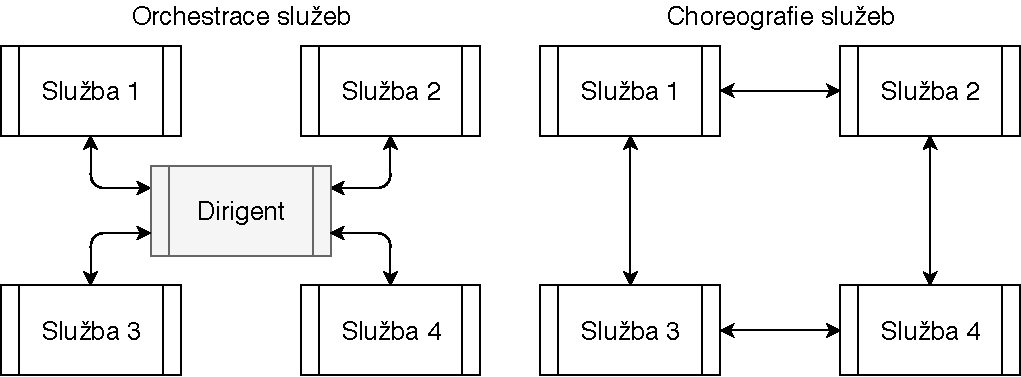
\includegraphics[keepaspectratio=true, width=0.8\linewidth]{figures/choreography-orchestration.pdf}
    \caption{Porovnán\'{\i} orchestrace a choreografie služeb}
    \label{fig:choreography-orchestration}
\end{figure}

\section{Nedostatky současného př\'{\i}stupu}

\goal{Navázán\'{\i} na předchoz\'{\i} sekci}
Jak jsme zjistili v předchoz\'{\i}ch odstavc\'{\i}ch, \gls{SOA} se zaměřuje zejména na
dělen\'{\i} systému na služby a detailně rozeb\'{\i}rá formu jejich vzájemné komunikace.
Neodpov\'{\i}dá ale na několik závažn\'ych otázek, se kter\'ymi se v praxi musej\'{\i}
architekti informačn\'{\i}ch systémů vypořádat, aby architektura byla schopná uspokojivě
plnit požadavky, které jsou na n\'{\i} kladené.

\goal{Problémy SOA a průřezov\'ych problémů}
Jelikož jedn\'{\i}m z c\'{\i}lů \gls{SOA}, potažmo microservices, je co nejv\'{\i}ce izolovat
jednotlivé služby, maj\'{\i} tyto architektury tendenci duplikovat části kódu
zajišťuj\'{\i}c\'{\i} funkcionalitu, která vyžaduje konzistentn\'{\i} zpracován\'{\i} ve v\'{\i}ce
službách~\cite{cerny2017disambiguation}, tzv. \textit{průřezov\'ych
problémů} (z anglického \textit{cross-cutting concerns}).
Př\'{\i}kladem mohou b\'yt právě byznysová pravidla~\cite{cemus2014aspect}, která je potřeba
zohlednit v rámci různ\'ych byznysov\'ych kontextů realizovan\'ych ve v\'{\i}ce službách.
Mezi dalš\'{\i} př\'{\i}klady se řad\'{\i} logován\'{\i}, monitoring či sběr dat
o telemetrii procesů.

\goal{Nast\'{\i}něn\'{\i} konkrétn\'{\i}ho př\'{\i}kladu}
Abychom si mohli lépe představit diskutovan\'y problém, znázorněmě
si ho na konkrétn\'{\i}m př\'{\i}kladu. Uvažme e-commerce systém
skládaj\'{\i}c\'{\i} se z několika služeb naprogramovan\'ych v různ\'ych technologi\'{\i}ch,
organizovan\'ych kolem jeho byznysov\'ych funkc\'{\i}.
Jedna služba obsluhuje byznysové operace vázaj\'{\i}c\'{\i}
se na uživatele systému, jejich registraci a administraci. Druhá
služba realizuje operace s produkty, jejich vytvářen\'{\i}, úpravu,
správu skladov\'ych zásob a informace o dostupnosti. Třet\'{\i} služba je
zodpovědná za vytvářen\'{\i} a správu objednávek, informován\'{\i} uživatelů
o změnách jejich stavů a vytvářen\'{\i} statistik a reportů pro management.
Čtvrtá služba má na starosti účetnictv\'{\i}, tedy vystavován\'{\i} a přij\'{\i}mán\'{\i}
faktur a komunikaci s bankovn\'{\i}mi službami o potvrzen\'{\i} přijat\'ych plateb.
Posledn\'{\i}, pátá služba, poskytuje uživatelské a umožňuje komfortn\'{\i} obsluhu systému.

\goal{Konkrétn\'{\i} problémy zpracován\'{\i} průřezov\'ych problémů na př\'{\i}kladu}
Jak již v\'{\i}me, každá byznysová operace má své preconditions, které musej\'{\i} b\'yt splněny,
aby mohla b\'yt vykonána. Operace má také post-conditions, které musej\'{\i} b\'yt
aplikovány po skončen\'{\i} operace. Např\'{\i}klad při vytvářen\'{\i} faktury za
objednávku mus\'{\i} b\'yt zvalidována fakturačn\'{\i} adresa, bez n\'{\i}ž nemůže
b\'yt faktura vystavena. Pokud chceme ušetřit práci účetn\'{\i}kům, kteř\'{\i} by
v př\'{\i}padě nevalidn\'{\i} adresy musely kontaktovat zákazn\'{\i}ka – pokud vůbec
takovou možnost maj\'{\i} – mus\'{\i}me tento fakt zohlednit již při vytvářen\'{\i} objednávky.
Proces vytvářen\'{\i} objednávky ale realizuje jiná služba, než vystavován\'{\i} faktur.
V ideáln\'{\i}m př\'{\i}padě bychom chtěli zákazn\'{\i}ka upozornit na nevalidn\'{\i} fakturačn\'{\i}
adresu dynamicky ještě před odeslán\'{\i}m objednávkového formuláře př\'{\i}mo v uživatelském
rozhran\'{\i}~\cite{cemus2017separation}. Pro lepš\'{\i} představu je problém znázorněn na
obrázku~\ref{fig:service-cutting},

\goal{Náročná údržba a reakce na změnu požadavku}
Z tohoto př\'{\i}kladu je jasně vidět, že stejná funkcionalita se prom\'{\i}tá
do tř\'{\i} služeb, z nichž každá má zodpovědnost za jiné byznysové operace.
To znamená, že stejn\'y kód, kter\'y realizuje validaci fakturačn\'{\i} adresy,
mus\'{\i} b\'yt implementován v každé ze služeb – v našem př\'{\i}padě nav\'{\i}c ve třech
různ\'ych programovac\'{\i}ch jazyc\'{\i}ch. Ve chv\'{\i}li, kdy vzejde požadavek na změnu
validace fakturačn\'{\i} adresy \textendash řekněme, že chceme zobecnit
validaci PSČ a umožn\'{\i}me přij\'{\i}mat i jeho tvar s mezerou – mus\'{\i}me stejnou změnu
provést konzistentně na třech různ\'ych m\'{\i}stech, všechny tři služby znovu
sestavit a nasadit ve správném pořad\'{\i} tak, aby nedošlo ke stavu,
kdy jedna služba přijme nov\'y tvar PSČ, ale navazuj\'{\i}c\'{\i} služba ho nen\'{\i}
schopna zpracovat.

\goal{Microservices neř\'{\i}ká nic o tom, jak velké je mikro}
Pozorn\'y čtenář může nam\'{\i}tnout, že problém validace fakturačn\'{\i}ch adres by
bylo možné vyřešit vyčleněn\'{\i}m této funkcionality
do samostatné služby a vystavit jej\'{\i} rozhran\'{\i} pro ostatn\'{\i} služby,
v souladu s nosnou myšlenkou microservices. Je pravda, že microservices
v názvu nese slovo \uv{micro} a evokuje tak, že služby by měly b\'yt co nejmenš\'{\i}
a nést co nejméně zodpovědnosti. Může ale nastat stav, kdy je služba př\'{\i}liš malá?
Pokud služby ponesou př\'{\i}liš málo odpovědnosti,
přináš\'{\i} to s sebou několik problémů, které je nutné zvážit. Mus\'{\i}me m\'{\i}t na paměti, že
nasazen\'{\i} a provoz každé služby s sebou přináš\'{\i} náklady nav\'{\i}c
a zvyšuje časové nároky na jejich v\'yvojáře a administrátory.
Komunikace služeb po s\'{\i}ti je nav\'{\i}c podstatně pomalejš\'{\i} a náchylnějš\'{\i} na
chybu, než komunikace jednotliv\'ych komponent v rámci jednoho procesu.
S rostouc\'{\i}m počtem \textit{průřezov\'ych problémů} by tak i rychle rostl
počet služeb v systému a celkové náklady na jeho v\'yvoj a údržbu.

\begin{figure}
    \centering
    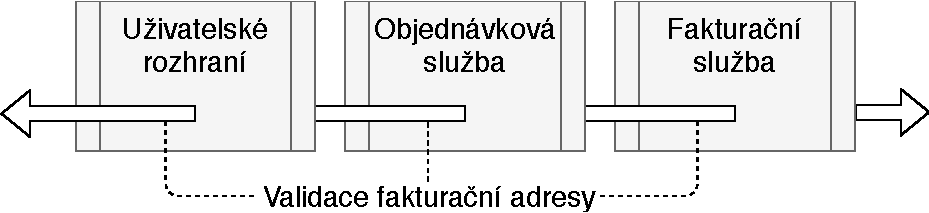
\includegraphics[keepaspectratio=true, width=0.8\linewidth]{figures/service-cutting.pdf}
    \caption{Př\'{\i}klad zásahu jedné funkcionality do v\'{\i}ce služeb}
    \label{fig:service-cutting}
\end{figure}

\goal{Shrnut\'{\i} problémů}
Na př\'{\i}kladu můžeme vidět, že existuje typ problémů, které v rámci architektury
orientované na služby při využit\'{\i} současného př\'{\i}stupu nejsme schopni uspokojivě
vyřešit na jednom m\'{\i}stě a vedou k duplikaci znalost\'{\i} na v\'{\i}ce m\'{\i}stech systému.
Taková duplikace může vést k zv\'yšenému riziku lidské chyby v\'yvojáře a t\'{\i}m k
nekonzistentn\'{\i}mu chován\'{\i} systému. Nav\'{\i}c zvyšuje cenu na v\'yvoj a údržbu systému.

\section{Identifikace požadavků na implementaci frameworku}\label{sec:implementation-requirements}

Z př\'{\i}kladu popsaného v\'yše můžeme identifikovat požadavky, které by měly
b\'yt zohledněny při návrhu a implementaci frameworku, kter\'y bude sloužit
pro centráln\'{\i} administraci a automatickou distribuci byznysov\'ych pravidel
v architektuře orientované na služby.

Framework, resp. jeho knihovny, by měly umožňovat:

\begin{itemize}
    \item{Definice byznys kontextů pomoc\'{\i} platformně nezávislého doménově specifického jazyka srozumitelného pro doménové experty}
    \item{Zápis preconditions a post-conditions pravidla jednotliv\'ych byznys kontextů}
    \item{Možnost jednoho kontextu rozšiřovat jiné kontexty}
    \item{Možnost centrálně spravovat byznysové kontexty, včetně úpravy stávaj\'{\i}c\'{\i}ch a vytvářen\'{\i} nov\'ych kontextů}
    \item{Automatickou distribuci kontextů, vyhodnocován\'{\i} jejich preconditions a aplikaci post-conditions}
    \item{Možnost využ\'{\i}vat framework na v\'{\i}ce plaformách}
\end{itemize}

\section{Shrnut\'{\i}}

V této kapitole jsme nast\'{\i}nili problematiku vysoké komplexity modern\'{\i}ch informačn\'{\i}ch systémů
a z toho vypl\'yvaj\'{\i}c\'{\i} požadavky na jejich architekturu. Analyzovali jsme koncept byznysov\'ych
pravidel a byznysov\'ych kontextů. Dále jsme prozkoumali architekturu orientovanou na služby, jej\'{\i}
v\'yhody a nev\'yhody, jej\'{\i} modern\'{\i} evoluci v podobě microservices a identifikovali jsme nedostatky
současn\'ych př\'{\i}stupů v řešen\'{\i} průřezov\'ych problémů, které zasahuj\'{\i} do v\'{\i}ce služeb najednou. Nakonec
jsme vyjmenovali požadavky, které by měl splňovat framework, jež bude v\'ystupem této práce.

\usepackage[T1]{fontenc}
\usepackage[utf8]{inputenc}

%!TEX ROOT=../diploma-thesis.tex

\chapter{Rešerše}\label{ch:reserse}

\section{Modelem řízená architektura}

\todo{
\begin{itemize}
    \item Co to je MDA
    \item Výhody
    \item Nevýhody
    \item Shrnutí a proč se nám nehodí
\end{itemize}
}

\section{Architektura klient-server}\label{sec:client-server}

\todo{
\begin{itemize}
    \item Co to je
    \item Výhody
    \item Nevýhody
    \item Shrnutí a proč se nám hodí
    \item Citovat ~\cite{berson1992client}
\end{itemize}
}

\section{Aspektově orientované programování}

\goal{Co je paradigma}
Programování je komplexní disciplína s teoreticky
neomezeným počtem možností, jakým programátor může
řešit zadaný problém. Ačkoliv každá úloha má své specifické
požadavky, za relativně krátkou historii programování se
stihlo ustálit několik ideologií, tzv. programovacích
paradigmat, které programátorovi poskytují sadu abstrakcí
a základních principů~\cite{van2009programming}.
Díky znalosti paradigmatu může programátor nejen zlepšit
svou produktivitu, ale zároveň může snáze pochopit myšlenky
jiného programátora a tím zlepšit kvalitu týmové spolupráce.

\goal{OOP a jeho popis}
Jedním z nejpopulárnějších paradigmat používaných k
vývoji moderních enterprise systémů je nepochybně
objektově orientované programování (OOP). To vnímá daný problém
jako množinu objektu, které spolu intereagují. Program
člení na malé funkční celky odpovídající struktuře
reálného světa~\cite{rentsch1982object}. Je vhodné zmínit,
že objekty se rozumí jak konkrétní koncepty, například
auto nebo člověk, tak i abstraktní koncepty,
namátkou bankovní transakce nebo objednávka v obchodě.
Objekty se pak promítají do kódu programu i do
reprezentace struktur v paměti počítače.
Tento přístup je velmi snadný pro pochopení,
vede k lepšímu návrhu a organizaci programu a snižuje
tak náklady na jeho vývoj a údržbu.

\goal{Nedostatky OOP}
Ačkoliv je OOP velmi silným a všestraným nástrojem,
existují problémy, které nelze jeho pomocí efektivně řešit.
Jedním takovým problémem jsou obecné požadavky na systém,
které musejí být konzistentně dodržovány na více místech,
které spolu zdánlivě nesouvisí. Příkladem
může být logování systémových akcí, optimalizace správy paměti
nebo uniformní zpracování výjimek~\cite{kiczales1997aspect}.
Takové požadavky nazýváme \textit{cross-cutting concerns}.
V rámci OOP je programátor nucen v ojektech manuálně opakovat
kód, který zodpovídá za jejich realizaci. Duplikace kódu
vede k větší náchylnosti na lidskou chybu a k vyšším nárokům na vývoj
a údržbu daného softwarového systému~\cite{fowler1999refactoring}.

\goal{AOP jako odpověď na nedostatky OOP}
Aspektově orientované programování (AOP) přináší řešení na
výše zmiňované problémy. Extrahuje obecné požadavky,
tzv. \textit{aspekty} do jednoho místa a pomocí procesu zvaného
\textit{weaving} je poté automaticky distribuuje do systému.
Weaving může proběhnout staticky při kompilaci programu nebo dynamicky
při jeho běhu. V obou případech ale programátorovi ulehčuje práci,
protože k definici i změně aspektu dochází centrálně a tím je eliminována
potřeba manuální duplikace kódu. Je nutno poznamenat, že AOP není
paradigmatem poskytujícím kompletní framework pro návrh programu.
V ideálním případě je tedy k návrhu systému využita kombinace
AOP s jiným paradigmatem. Pro účely této práce se zaměříme na
kombinaci AOP a OOP.

\todo{
\begin{itemize}
    \item diagram cross cutting concerns
    \item roztáhnout do více odstavců
    \item diagram weaveru
    \item section BPEL
\end{itemize}
}

\begin{description}
    \item [Aspekt]
    \item [Join-point]
    \item [Pointcut]
    \item [Advice]
    \item [Weaving]
\end{description}

\section{Aspect-driven Design Approach}

\todo{
\begin{itemize}
    \item co to je
    \item jak nám to pomůže
    \item využítí jeho konceptů
    \item shrnutí
\end{itemize}
}

Aspect-driven Design Approach (ADDA)

\goal{Vhodnost AOP pro náš úkol}
Vzhledem k požadavkům na implementaci našeho frameworku stanoveným
v předchozí kapitole~\ref{ch:analyza} se AOP a na něm stavějící ADDA
jeví jako vhodný přístup, který nám pomůže dosáhnout cíle.

\section{Stávající řešení reprezentace business pravidel}

\subsection{Drools DSL}

\todo{
\begin{itemize}
    \item co to je
    \item jak to funguje
    \item výhody
    \item nevýhody
    \item shrnutí a proč se nám nehodí
\end{itemize}
}

\goal{Drools se nám nehodí, protože je jen pro platformu Java}
...

\subsection{JetBrains MPS}

\todo{
\begin{itemize}
    \item co to je
    \item jak to funguje
    \item výhody
    \item nevýhody
    \item shrnutí a proč se nám nehodí
\end{itemize}
}

\goal{MPS je super, ale nevyhovuje nám kvůli dynamickým změnám}
...

\section{Shrnutí}

V této kapitole jsme provedli rešerši \textit{architektury orientované
na služby}, jejích výhod, nevýhod a známých nedostatků. Dále jsme
prozkoumali, jaký způsobem funguje síťová \textit{architektura klient-server},
jaké jsou výhody a nevýhody \textit{modelem řízeného vývoje} pro náš případ
a shrnuli jsme paradigma \textit{aspektově orientovaného programování} a
z něch vycházející přístup k návrhu softwarových systémů \textit{ADDA}.
Nakonec jsme provedli rešerši stávajících řešení reprezentace byznys pravidel
včetně komplexního frameworku \textit{Drools} a zhodnotili jsme jeho vhodnost
k řešení našeho problému.

%!TEX ROOT=../diploma-thesis.tex

\chapter{Návrh frameworku}\label{ch:navrh}

V této kapitole je diskutován návrh frameworku pro centrální správu
a automatickou integraci business pravidel vyhovující požadavkům identifikovaným
v sekci~\ref{sec:implementation-requirements}. Tento návrh staví na znalostech získaných
v předchozí kapitole~\ref{ch:reserse}, zejména na paradigmatu \gls{AOP} a přístupu \gls{ADDA}.

\section{Formalizace architektury orientované na služby}

Pro formalizaci problému byznysových pravidel v \gls{SOA} do termínů \gls{AOP} je nutno
identifikovat \textit{join-points}, určit podobu \textit{advices}, popsat způsob jakým budou
zachyceny \textit{pointcuts} a nakonec navrhnout proces \textit{weavingu} pravidel.

\subsection{Join-points}

Identifikace join-points vychází ze životního cyklu služby, který je znázorněn
na obrázku~\ref{fig:join-points}. První fází v životě instance služby je její inicializace,
konkrétně načtení aplikačního kontextu. V tomto bodě je potřeba získat veškerá pravidla, která
bude služba potřebovat ke své funkci.
Po inicializaci vstupuje služba do fáze, ve které může přijímat požadavky
na vykonání byznysových operací. Při přijmutí požadavku je nejprve nutno určit
byznysový kontext a poté vyhodnotit veškeré \textit{preconditions}. Pokud jsou všechny předpoklady
pro spuštění operace splněny, může být vykonána. Po dokončení operace je nutno aplikovat relevantní
post-conditions.

\begin{figure}
    \centering
    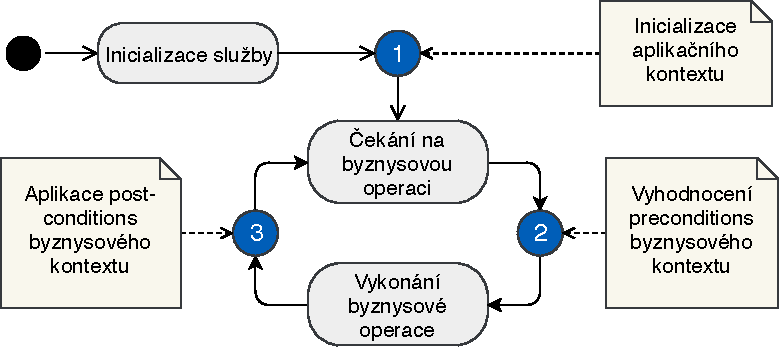
\includegraphics[keepaspectratio=true, width=0.6\linewidth]{figures/join-points.pdf}
    \caption{Diagram životn\'{\i}ho cyklu služby a identifikovan\'ych join-pointů}
    \label{fig:join-points}
\end{figure}

Identifikované join-points tedy jsou:

\benum[label=\circledarabic]
\item\label{itm:initialization} Inicializace instance služby
\item\label{itm:before} Volání byznysové operace
\item\label{itm:after} Dokončení byznysové operace
\eenum

\subsection{Pointcuts}

V join-pointu~\ref{itm:initialization} by služba měla načíst všechna byznysová pravidla, která
bude potřebovat ke své činnosti, a nejsou pro ni lokálně dostupná. Služba tedy musí zjistit,
která pravidla je potřeba získat, a následně si je vyžádat od ostatních služeb.
V join-pointech~\ref{itm:before}~a~\ref{itm:after} musejí být aplikována byznysová pravidla každého
kontextu vztahujícího se k dané operaci.

\lstinputlisting[
caption={Ukázka zápisu validačních pravidel pomocí anotací v jazyku Java},
label={lst:jsr303},
language=Java,
%frame=single,
%float,
%floatplacement=t
]
{code/jsr303.java}

Pro zápis selektoru poincutu byznysového pravidla se lze inspirovat standardem \gls{JSR}
303~\cite{bernard2009jsr}, který umožňuje validovat data byznysových objektů vstupujících do
byznysových operací pomocí anotací atributů těchto objektů. Příklad validačních anotací je znázorněn
ve zdrojovém kódu~\ref{lst:jsr303}, kde je pomocí anotace \code{$@$NotNull} zajištěno, že fakturační
adresa bude mít vyplněna všechna pole (v kontextu našeho frameworku se jedná o paralelu preconditions).
Podobným způsobem by každá byznysová operace mohla pomocí metainstrukcí specifikovat, která byznysová
pravidla bude využívat. Toto řešení však neposkytuje možnost dynamicky při běhu programu změnit sadu
byzynsových pravidel. Tento problém lze řešit zavedením konceptu byznysového kontextu, který
zapouzdřuje byznysová pravidla, a byznysová operace se na něj může explicitně odkázat. Obsah byznysového
kontextu by přitom mohl být dynamicky změněn za běhu programu.

Sdílení pravidel mezi byznysovými kontexty, potažmo byznysovými operacemi a mezi jednotlivými službami,
by lze realizovat pomocí dědičnosti kontextů. Každý kontext, který by potřeboval validovat fakturační
adresu, by tak mohl pouze dědit od kontextu vytváření faktury. Na obrázku~\ref{fig:context-extension}
je dědičnost kontextů znázorněna. Kontext vytváření objednávky dědí od kontextu vytváření faktury
a znovupoužívá jeho byznysová pravidla. Byznysové operace se odkazují na byznysové kontexty, které mají
být při jejich vykonávání použity. Před spuštěním a po dokončení operace vytváření
objednávky jsou aplikována pravidla obou kontextů, zatímco při vytváření faktury jsou zohledněna
pouze pravidla jednoho kontextu.

\begin{figure}
    \centering
    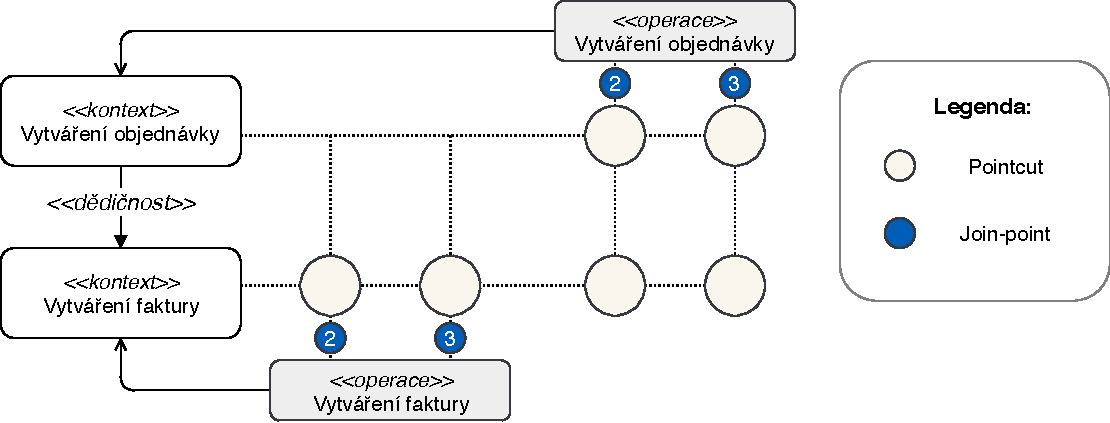
\includegraphics[keepaspectratio=true, width=1\linewidth]{figures/context-extension.pdf}
    \caption{Dědičnost kontextů ve vztahu k join-pointům a pointcuts}
    \label{fig:context-extension}
\end{figure}

\subsection{Advices}

V případě join-pointu~\ref{itm:initialization} je advice samotná reprezentace byznysového
kontextu přenášeného mezi službami. Naopak v join-pointech~\ref{itm:before}~a~\ref{itm:after}
je přidanou funkcionalitou vyhodnocování preconditions nad aplikačním kontextem, resp. aplikování
post-conditions na návratovou hodnotu operace.

\subsection{Weaving}

Weaving v případě join-pointu~\ref{itm:initialization} bude provádět komponenta frameworku, která
analyzuje lokálně dostupná pravidla služby, vyhodnotí, která pravidla je potřeba stáhnout,
a vyžádá tato pravidla od příslušných služeb.
V případě join-pointů~\ref{itm:before}~a~\ref{itm:after} je k weavingu potřeba využít speciální aspect
weaver. Ten zachytí volání byznysové operace a získá informace o aktuálním stavu aplikačního kontextu.
Následně zjistí, který byznysový kontext má být aplikován, shromaždí všechny preconditions
a každou z nich vyhodnotí. Pokud některá precondition není splněna, byznysová operace je zastavena
a je vyhozena výjimka, kterou služba zpracuje. V opačném případě je kontrola vrácena zpět
službě, která vykoná byznysovou operaci. Po dokončení operace aspect weaver zachytí výstup byznysové
operace a aplikuje post-conditions daného byznysového kontextu. Proces weavingu je zachycen na
obrázku~\ref{fig:business-rules-weaver}.

\begin{figure}
    \centering
    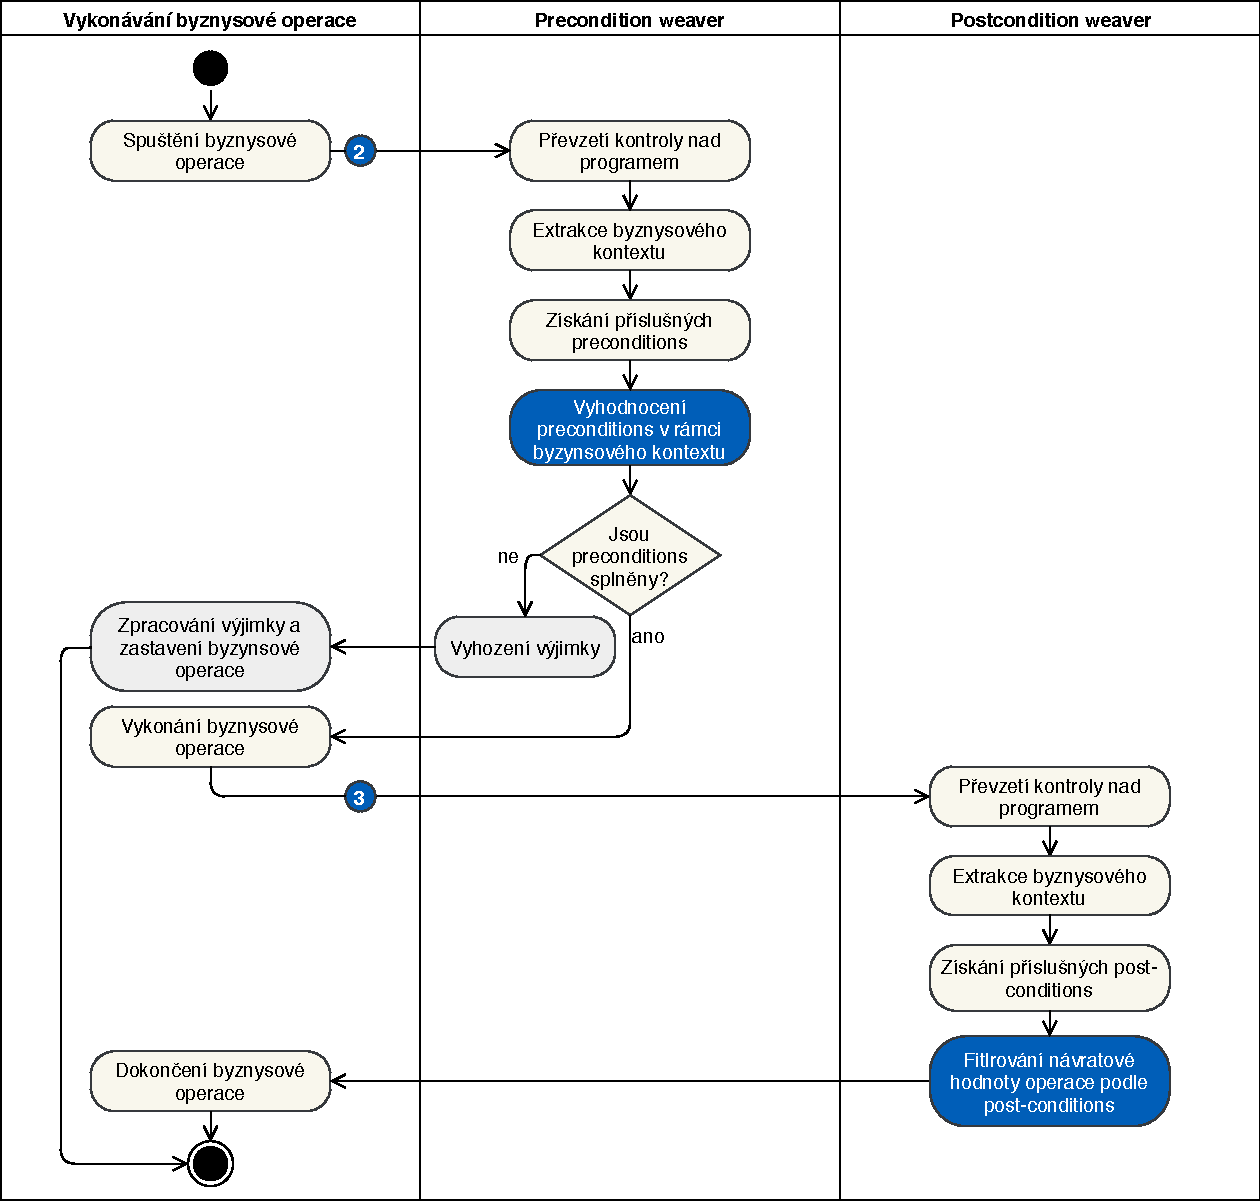
\includegraphics[keepaspectratio=true, width=0.8\linewidth]{figures/business-rules-weaver.pdf}
    \caption{Proces weavingu byznysov\'ych pravidel}
    \label{fig:business-rules-weaver}
\end{figure}

\section{Dědičnost byznysových kontextů}\label{sec:context-inheritance}

V předchozím textu byl představen koncept dědičnosti byznysových kontextů.
Každý kontext díky němu může rozšiřovat libovolné množství jiných kontextů, a sdílet jejich
byznysová pravidla. Byznysové operace pak mohou samy určit, který byznysový kontext se k ním váže.
Tento kontext však přináší několik problémů, které jsou rozebrány v následujících odstavcích.

Může nastat situace, kdy je potřeba sdílet pouze některá byznysová pravidla
daného kontextu. Při mapování kontextů jedna ku jedné s operacemi by to ale
nebylo možné. Řešením je využití tzv. \textit{abstraktních kontextů},
které přímo nevyužívá žádná byznysová operace.
Příklad znázorněný na obrázku~\ref{fig:abstract-context} popisuje situaci, kdy je nežádoucí,
aby kontext \code{user.register} zdědil pravidlo vyžadující přihlášení uživatele.

\begin{figure}
    \centering
    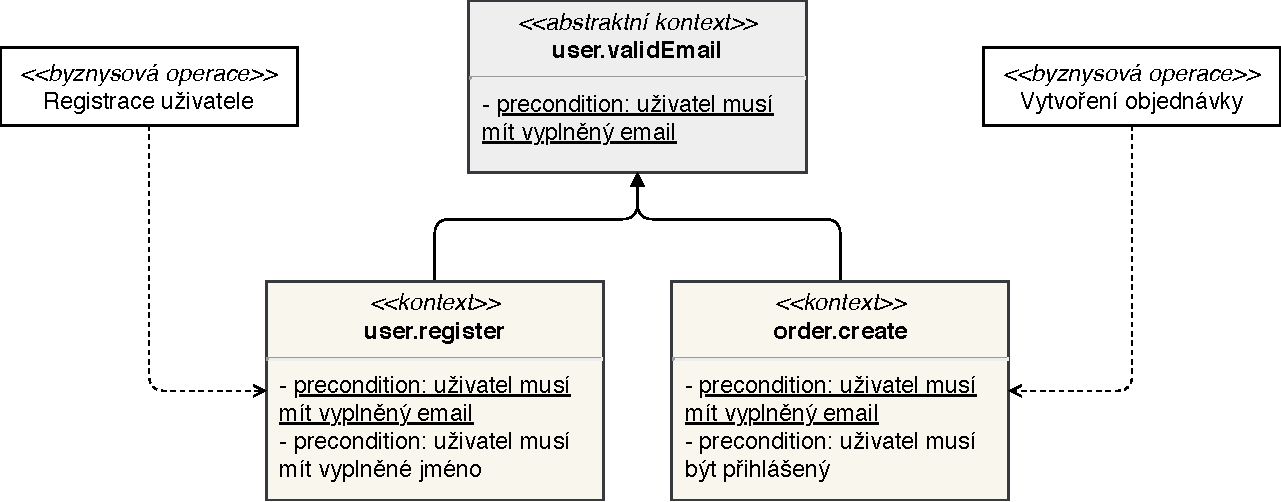
\includegraphics[keepaspectratio=true, width=1\linewidth]{figures/abstract-context.pdf}
    \caption{Znázornění abstraktního byznysového kontextu}
    \label{fig:abstract-context}
\end{figure}

Kvůli dědičnosti může vzniknout v grafu závislostí kontextů cyklus, který by způsobil zacyklení
procesu inicializace v~\ref{itm:initialization}. Tuto situaci nelze z hlediska frameworku vyřešit,
ale dá se jí předejít. K prevenci by mohl sloužit validátor vestavěný do nástroje pro správu
byznysových kontextů.

Vícenásobná dědičnosti může přinést problém, kdy jeden kontext zdědí více stejných pravidel z
různých zdrojů, tzv. \textit{diamond problem}~\cite{boyen1994generalized}. Tomu lze předejít tak, že
každé pravidlo bude mít unikátní identifikátor v rámci celého systému a při dědění budou zohledněna
pouze unikátní pravidla. Zajištění unikátního identifikátoru lze zajistit díky nástroji pro centrální
administraci byznysových pravidel.

\section{Logické výrazy byznysových pravidel}

Sekce~\ref{sec:business-rules} uvádí, že pravidla obsahují logické podmínky. V případě preconditions je to
ověření podmínky, která musí být platná před spuštěním byznysové operace v~\ref{itm:before}. V případě
post-condition může filtrování návratové hodnotry podléhat splnění určité podmínky, která musí být
vyhodnocena v~\ref{itm:after}.

\begin{figure}
    \centering
    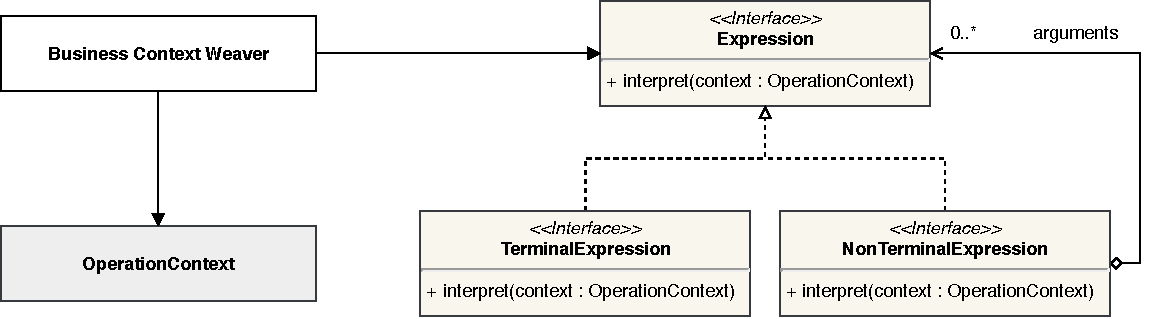
\includegraphics[keepaspectratio=true, width=1\linewidth]{figures/expression.pdf}
    \caption{Použití vzoru Intepreter pro vyhodnocování logických výrazů}
    \label{fig:expression}
\end{figure}

Podmínky byznysových pravidel se skládají z jednotlivých výrazů, které tvoří
orientovaný acyklický graf (\gls{DAG}), tzv. \textit{derivační strom}.
Výrazy se dělí na \textit{terminály} a \textit{neterminály}~\cite{melichar2003jazyky}.
Terminál znamená, že z daného výrazu již nevychází žádná hrana do jiného výrazu.
Neterminál je opak terminálu. Pro reprezentaci stromu bude využit návrhový vzor
\textit{Composite}~\cite{fowler2002patterns}. K vyhodnocování podmínek popsaných v byznysovém
pravidle je vhodný návrhový vzor \textit{Interpreter}~\cite{fowler2002patterns}, jehož
použití je demonstrováno na obrázku~\ref{fig:expression}.

Framework bude disponovat základní sadou výrazů pro zápis byznysových pravidel.
Mezi ně budou patřit logické operace \code{and}, \code{or}, \code{equals} a \code{negate}.
Dále výraz \code{VariableReference}, který získá hodnotu proměnné či konstanty z kontextu.
Pokud bude v kontextu uložen objekt, je potřeba přistupovat i k jeho
veřejným atributům, což bude zajišťovat výraz \code{ObjectPropertyReference}.
K ověření přítomnosti hodnoty v proměnné bude sloužit výraz \code{IsNotNull}. Výraz \code{IsNotBlank} ověří,
zda je v proměnné řetězec nenulové délky. Pro vložení konstantní hodnoty přímo do byznysového pravidla bude
sloužit terminál \code{Constant}. Pro zvýšený komfort budou přidány i výrazi realizující základní matematické operace sčítání, odečítání,
násobení a dělení. Pro volání uživatelských funkcí definovaných v operačním kontextu bude sloužit speciální výraz
\code{FunctionCall}. V jeho případě je nutno zohlednit skutečnost, že funkce může přijímat libovolný počet argumentů.
Protože volaná funkce může potřebovat přistupovat k operačnímu kontextu, musejí být argumenty také interpretovány.
Bohužel nelze u uživatelem definovaných funkcí ověřit, že bude při jejich volání odpovídat počet a typ argumentů.
Přehled všech výrazů, které bude framework podporovat, je v tabulce~\ref{tbl:expressions},

\afterpage{%
\clearpage% Flush earlier floats (otherwise order might not be correct)
\begin{landscape}
    \begin{table}
        \centering
        \begin{tabular}{ l l l c c }
            \hline
            \textbf{Název} & \textbf{Argumenty} & \textbf{Atributy} & \textbf{Návratový typ} & \textbf{Typ výrazu} \\ \hline \hline
            \textbf{Constant} & - & Hodnota a typ konstanty & \code{?} & Terminál \\
            \textbf{FunctionCall} & Libovolný počet argumentů & Návratový typ funkce & \code{?} & Terminál \\
            \textbf{IsNotNull} & Jeden argument libovolného typu & - & \code{BOOL} & Neterminál \\
            \textbf{IsNotBlank} & Jeden argument typu \code{STRING} & - & \code{BOOL} & Neterminál \\
            \textbf{LogicalAnd} & 2 argumenty typu \code{BOOL} & - & \code{BOOL} & Neterminál \\
            \textbf{LogicalEquals} & 2 argumenty libovolného typu & - & \code{BOOL} & Neterminál \\
            \textbf{LogicalNegate} & 1 argument typu \code{BOOL} & - & \code{BOOL} & Neterminál \\
            \textbf{LogicalOr} & 2 argumenty typu \code{BOOL} & - & \code{BOOL} & Neterminál \\
            \textbf{NumericAdd} & 2 argumenty typu \code{NUMBER} & - & \code{NUMBER} & Neterminál \\
            \textbf{NumericSubtract} & 2 argumenty typu \code{NUMBER} & - & \code{NUMBER} & Neterminál \\
            \textbf{NumericMultiply} & 2 argumenty typu \code{NUMBER} & - & \code{NUMBER} & Neterminál \\
            \textbf{NumericDivide} & 2 argumenty typu \code{NUMBER} & - & \code{NUMBER} & Neterminál \\
            \textbf{ObjectReference} & - & Název objektu a název a typ proměnné & \code{?} & Terminál \\
            \textbf{VariableReference} & - & Název a typ proměnné & \code{?} & Terminál \\
            \hline
        \end{tabular}
        \caption{Přehled výrazů pro zápis byznysového pravidla}
        \label{tbl:expressions}
    \end{table}
\end{landscape}
\clearpage% Flush page
}

%\goal{Typované výrazy}
Pro snažší implementaci na více platformách a prevenci sémantických chyb v pravidlech budou výrazy
obsahovat i explicitní definici svého návratového typu. Výraz byznysového pravidla může nabývat logických hodnot,
může vracet číslo, textový řetězec a také objekt. Je potřeba počítat také s tím, že výraz nevrací žádnou
hodnotu.

\begin{itemize}
    \item \code{BOOL} je logický typ, který nabývá hodnoty \code{true} a \code{false}.
    \item \code{NUMBER} je reálné číslo zapsáno ve tvaru s desetinnou tečkou a neomezeným počtem číslic.
    \item \code{OBJECT} je objekt libovolného typu.
    \item \code{STRING} je textový řetězec.
    \item \code{VOID} je pseudotyp značící, že výraz nemá návratovou hodnotu.
\end{itemize}

%\goal{Atributy pravidel}
Kromě argumentů neterminálů je v některých případech potřeba k výrazu uložit i dodatečné informace \textendash\xspace
\textit{atributy}. Jedním z atributů je typ návratové hotnoty výrazu, pokud není přímo implikována.
V případě výrazu \code{Constant} je potřeba uložit hodnotu a typ konstanty. Reference na proměnnou
musí obsahovat její název a typ, reference na pole objektu navíc musí obsahovat název odkazovaného pole.
Volání funkce musí obsahovat její název a návratový typ.

\begin{figure}
    \centering
    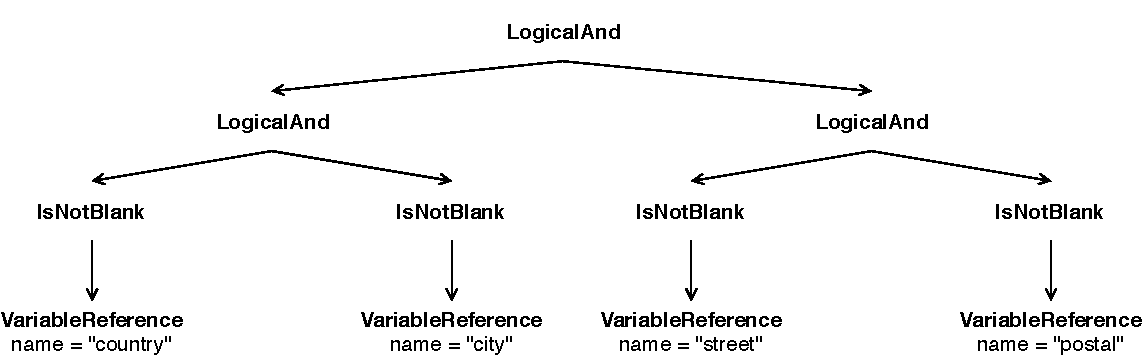
\includegraphics[keepaspectratio=true, width=1\linewidth]{figures/simple-rule.pdf}
    \caption{Syntaktický strom jednoduchého validačního pravidla}
    \label{fig:simple-rule}
\end{figure}

%\goal{Příklad AST pravidla}
Na obrázku~\ref{fig:simple-rule} je znázorněn syntaktický strom, který zachycuje jednoduché
validační pravidlo validující fakturační adresu. Jedná se o ekvivalent validačních pravidel
zachycených ve zdrojovém kódu~\ref{lst:jsr303} pomocí anotací standardu \gls{JSR} 303.
Pravidlo je tvořeno čtyřmi teminály, které se odkazují na proměnné operačního kontextu.
Hodnoty proměnných jsou validovány výrazem \code{IsNotBlank} a jednotlivé validace
jsou spojeny pomocí binárních výrazu \code{LogicalAnd} odpovídajících logické konjunkci.

\section{Filtrování návratových hodnot byznysové operace}

Při aplikování post-conditions je filtrována návratová hodnota byznysové operace. Tou může být proměnná
obsahující číslo, text, objekt, či jejich kolekce. Filtrování jednoduchých hodnot nemá pro byznysová pravidla reálný přínos.
V případě objektu lze filtrovat jeho atributy, například skrýt e-mailovou adresu uživatele.
V případě kolekce lze filtrovat jejich prvky, například skrýt objednávky, které uživateli nepatří.
Pokud se v kolekci nachází objekty, lze požadovat, aby byly zakryty atributy jednotlivých objektů,
například filtrování e-mailových adres v kolekci více uživatelů. Itentifikovanými typy post-conditions tedy jsou:

\begin{itemize}
    \item \code{FILTER\_OBJECT\_FIELD} filtruje atribut objektu, který je výstupem operace.
    \item \code{FILTER\_LIST\_OF\_OBJECTS} filtruje objekty v kolekci, která je výstupem operace.
    \item \code{FILTER\_LIST\_OF\_OBJECTS\_FIELDS} filtruje atributy objektů v kolekci, která je výstupem operace.
\end{itemize}

\section{Metamodel byznysového kontextu}\label{sec:metamodel}

\begin{figure}
    \centering
    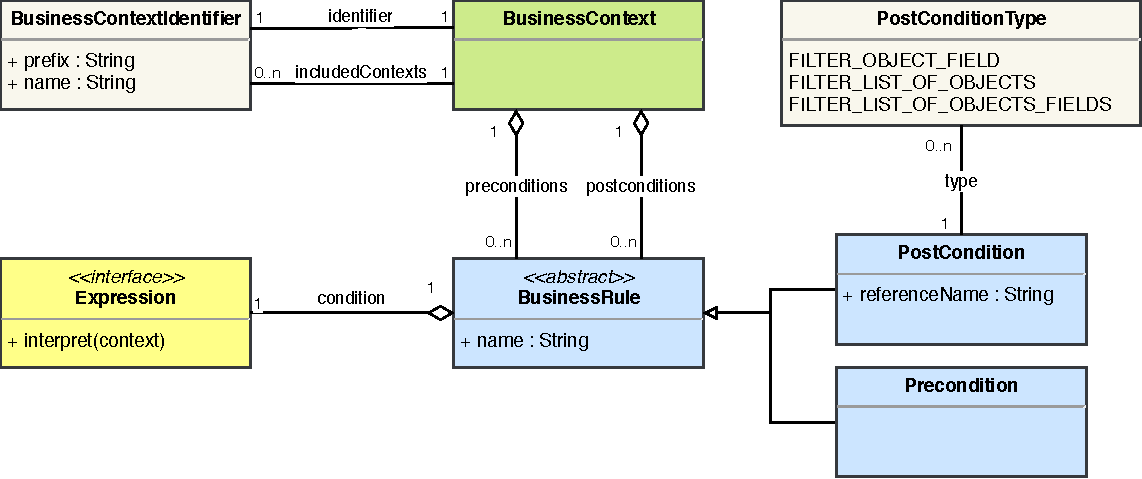
\includegraphics[keepaspectratio=true, width=\linewidth]{figures/business-context-metamodel.pdf}
    \caption{Metamodel byznysového kontextu}
    \label{fig:business-context-metamodel}
\end{figure}

Z předchozího textu vyplývá podoba metamodelu byznysových pravidel, resp. byznysových kontextů.
Kromě samotných logických výrazů musí pravidlo nést informace o tom, zda
se jedná o precondition nebo post-condition, a také jeho identifikátor.
Post-condition navíc potřebuje uložit informaci o jejím typu a názvu. Pravidla jsou uskupována
do byznysových kontextů, z nichž každý má svůj unikátní identifikátor skládající se z prefixu
a samotného jména a seznam rozšířených kontextů. Diagram tříd navrženého kontextu je znázorněn
na obrázku~\ref{fig:business-context-metamodel}.

\section{Popis byznysových kontextů pomocí \gls{DSL}}

Př\'{\i}stup \gls{ADDA} doporučuje popsat byznysová pravidla pomoc\'{\i}
vlastn\'{\i}ho, na m\'{\i}ru šitého, doménově specifického jazyka~\cite{cemus2015automated}.
Pro účely frameworku bude popsán pomocí \gls{DSL} celý byznysový kontext.
Jak bylo popsáno v sekci~\ref{sec:business-rule-dsl}, vlastnosti nástrojů Drools a JetBrains MPS,
nejsou optimální pro dosažení vytyčených cílů. Pro účely frameworku je tedy nutné specifikovat vlastnosti,
které by \gls{DSL} mělo nést. Konkrétní podoba DSL bude přenechána na implementaci frameworku.

Pro uložení kontextu z metamodelu do \gls{DSL}, aby ho mohl vývojář či administrátor
systému upravovat, je vzhledem k reprezentaci logických výrazů vhodný návrhový vzor
\textit{Visitor}~\cite{fowler2002patterns}. Ten umožní převádět libovolně složité logické
výrazy pomocí metody \textit{double-dispatch}. Jeho volbou je zároveň zajištěna rozšiřitelnost
frameworku pro libovolné \gls{DSL} \textendash\xspace bude stačit implementovat konkrétní
visitor pro zvolený jazyk, aniž by bylo nutno zasahovat přímo do implementace frameworku.
Princip použití vzoru Visitor je znázorněn na obrázku~\ref{fig:expression-visitor}.

\begin{figure}
    \centering
    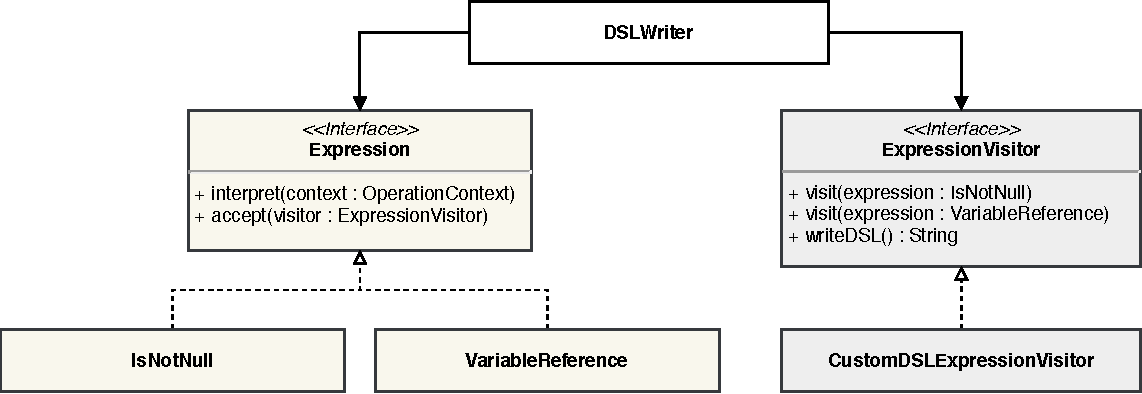
\includegraphics[keepaspectratio=true, width=1\linewidth]{figures/expression-visitor.pdf}
    \caption{Využití vzoru Visitor pro zápis logických výrazů v \gls{DSL}}
    \label{fig:expression-visitor}
\end{figure}

\section{Organizace byznysových kontextů}

Každá služba bude mít lokálně uložen popis byznysových kontextů, které se sémanticky vztahují
k její doméně. Pro snažší přidělení byznysových kontextů ke službám bude v identifikátoru kontextu sloužit
tzv. \textit{prefix}. Kontexty se stejným prefixem pak budou spravovány výhradně jednou službou. Například kontexty
služby spravující objednávky budou označeny prefixem \code{order}, zatímco kontexty služby zajišťující fakturaci budou
označeny prefixem \code{billing}. Může nastat i situace, kdy jedna služba bude spravovat více prefixů.

\subsection{Registr byznysových kontextů}

Cílem frameworku je soustředit byznysové kontexty na jedno místo, ze kterého budou
automaticky distribuovány. Pro tento účel bude využit registr byzynsových pravidel
(\code{BusinessContextRegistry}), který bude mít za úkol kontexty načítat z \gls{DSL} do metamodelu,
stahovat lokálně nedostupné kontexty z ostatních služeb a načtené kontexty uchovávat pro použití při weavingu.
Každá služba pak bude disponovat svým registrem. Při inicializaci kontextů spolu budou registry komunikovat
a vyměňovat si sdílené kontexty.

\subsection{Uložení kontextů}

Byznysové kontexty popsané pomocí \gls{DSL} mohou být v příslušné službě uloženy v souborech na disku či v
databázi. Navrhovaný framework by na způsobu uložení neměl být závislý a o potřebné kroky
pro načtení či případně uložení kontextu se postará konkrétní implementace. Pro tento účel
je tedy vhodné, aby registr pracoval s nekonkrétními rozhraními, na jejichž implementaci
nebude nijak záviset.

\section{Inicializace byznysových kontextů}

\begin{figure}
    \centering
    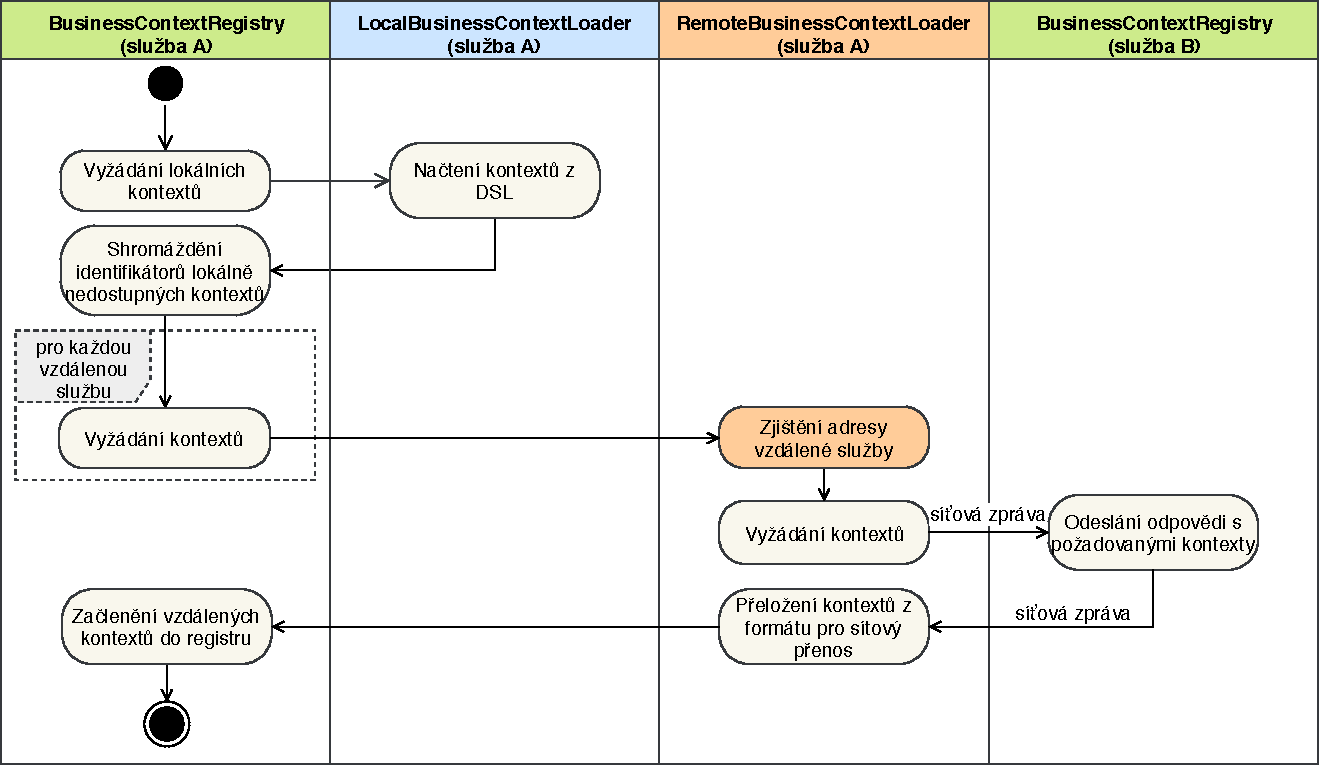
\includegraphics[keepaspectratio=true, width=\linewidth]{figures/business-context-loading.pdf}
    \caption{Proces inicializace byznysov\'ych kontextů}
    \label{fig:business-context-loading}
\end{figure}

Při inicializiaci byzynsových kontextů jsou nejprve načteny lokálně dostupné kontexty popsané pomocí \gls{DSL}.
Po převedení kontextů z \gls{DSL} do metamodelu je shromážděn seznam rozšířených kontextů a z nich jsou vybrány ty,
které nejsou lokálně dostupné. Následně jsou tyto vzdálené kontexty vyžádány od příslušných služeb
a po obdržení jsou převedeny ze síťového formátu do metamodelu. Nakonec jsou sdílená pravidla rozšířených kontextů začleněna
do kontextů, které od nich dědí. Celou inicializaci bude zastřešovat komponenta \code{BusinessContextRegistry}, která
má znalost o všech subsystémech, které jsou k tomuto procesu potřeba. Tato komponenta implementuje
návrhový vzor \textit{Facade}~\cite{fowler2002patterns}. Na obrázku~\ref{fig:business-context-loading} je znázorněn
navržený proces inicializace.

\section{Centráln\'{\i} správa byznysových kontextů}

Vzhledem k nutnosti centralizovat správu byznysových kontextů se
architektura \gls{P2P} představená v sekci~\ref{sec:p2p} nehodí.
Při úpravě kotextů by totiž v systému mohly existovat najednou staré i nové verze
byznysových pravidel, což je pro správnou funkci systému nepřijatelné.
Framework tedy využije architektury klient-server s více servery.
Byznysové kontexty budou podle prefixu přideleny službám, které budou
spravovat jejich aktuální a jediný stav a poskytovat je jiným službám.

\subsection{Uložen\'{\i} rozšířeného pravidla}\label{sec:saving-context}

Při ukládání byznysového kontextu je potřeba změnu propagovat do všech ostatních kontextů, které od něj dědí.
Při změně rozšířeného kontextu budou všechny služby, které ho využívají, informovány pomocí nástroje pro
centrální správu byzynsových pravidel. Ten má informaci o všech závislostech v systému a zároveň zná i adresu všech
služeb. Nevýhodou tohoto přístupu je zvýšená komunikační zátěž kvůli většímu objemu přenesených informací, stejný kontext
je totiž potřeba rozeslat mezi více služeb. Při implementaci je nutno zvážit, zda je tato zátěž vůči absolutnímu objemu
přenášených dat v systému významná. Bylo by vhodné vybrat vhodný přenosový formát, který minimalizuje dopad veškeré síťové
komunikace týkající se distribuce byznysových pravidel.

\subsection{Proces úpravy kontextu}

\begin{figure}
    \centering
    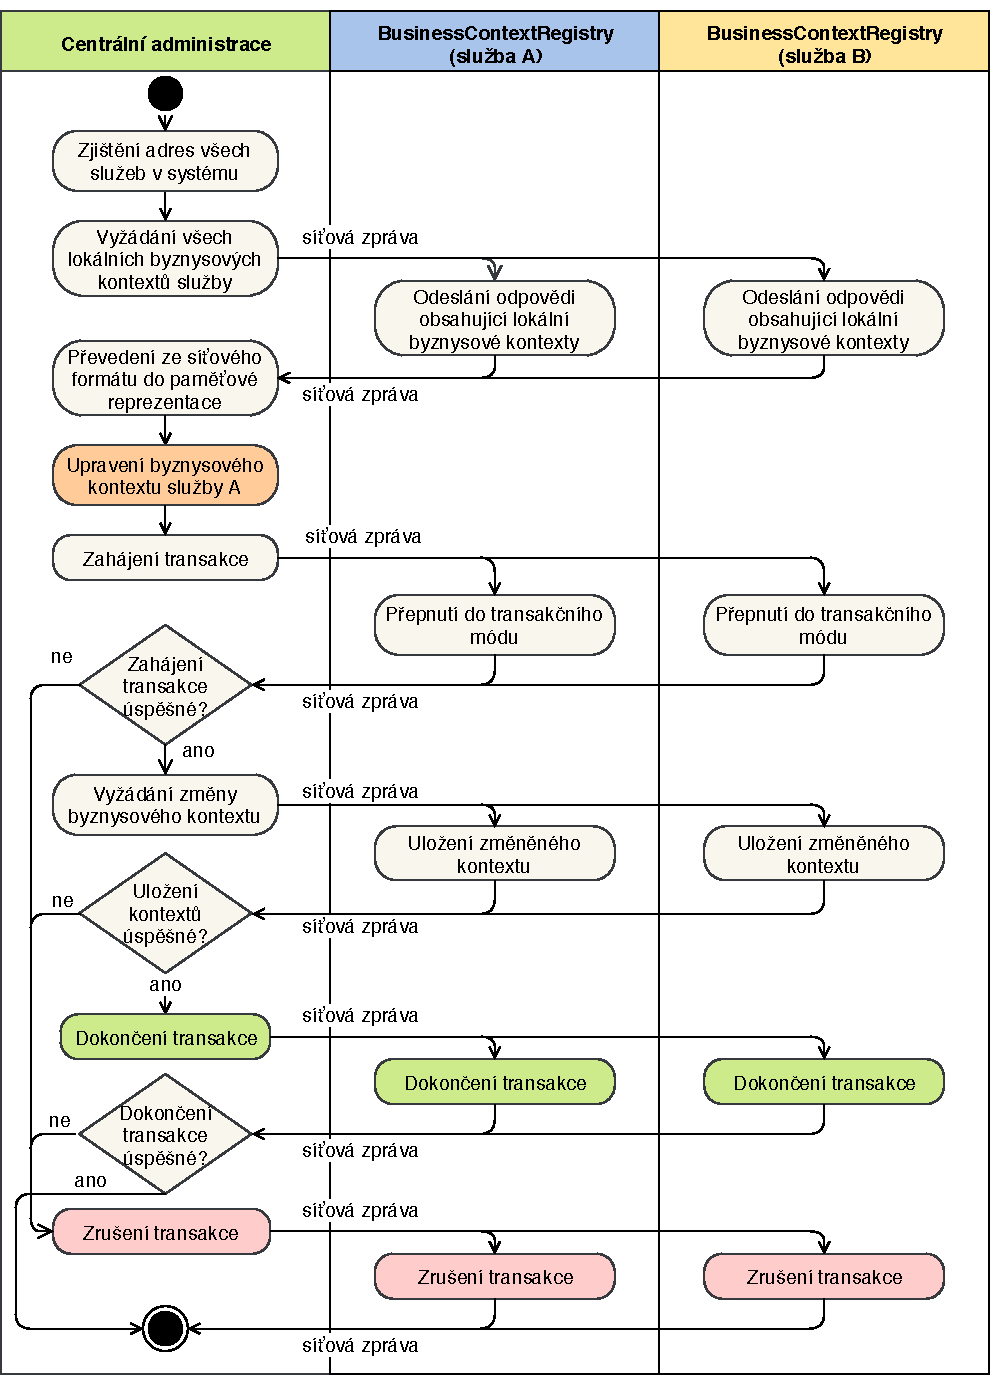
\includegraphics[keepaspectratio=true, width=\linewidth]{figures/business-context-management.pdf}
    \caption{Proces centráln\'{\i} správy byznysov\'ych kontextů}
    \label{fig:business-context-management}
\end{figure}

Proces úpravy byznysového kontextu pomocí nástroje pro centrální administraci nejprve načte všechny
byznysové kontexty všech služeb v systému. Následně zobrazí administrátorovi formulář pro úpravu pravidla.
Pravidlo je pro účely formuláře převedeno z metamodelu do \gls{DSL}. Po odeslání formuláře bude pravidlo
převedeno zpět do metamodelu. Nástroj pro administraci poté analyzuje, na které služby bude
mít změna pravidla dopad. Následně je s těmito službami zahájena transakce, při které v nich
nesmí probíhat žádná byznysová operace. Když všechny ovlivněné služby zahájí transakci, je možno
jim rozeslat novou podobu pravidla. Pokud vše proběhne v pořádku, je možno transakci dokončit
a služby otevřít byznysovým transakcím. Pokud naopak některý z kroků transakce selže, je nutno
informovat všechny zúčastněné služby o zrušení transakce a změnu inkriminovaného pravidla zrušit.
Na obrázku~\ref{fig:business-context-management} je celý proces znázorněn. Proces pro uložení
nového kontextu je analogický.

\section{Architektura frameworku}\label{sec:architecture}

V této sekci je popsána obecná architektura navrženého frameworku v rámci služby využívající
klasickou třívrstvou architekturu~\cite{fowler2002patterns}, která se skládá z prezentační,
aplikační a datové vrstvy. Každá z těchto vrstev může framework využívat
\textendash\xspace prezentační vrstva při validování vstupních polí formuláře, aplikační vrstva při
aplikaci byzynsových pravidel v byznysových operacích a datová vrstva při aplikaci post-conditions pro
filtrování dat při jejich získávání z databáze.

\begin{figure}
    \centering
    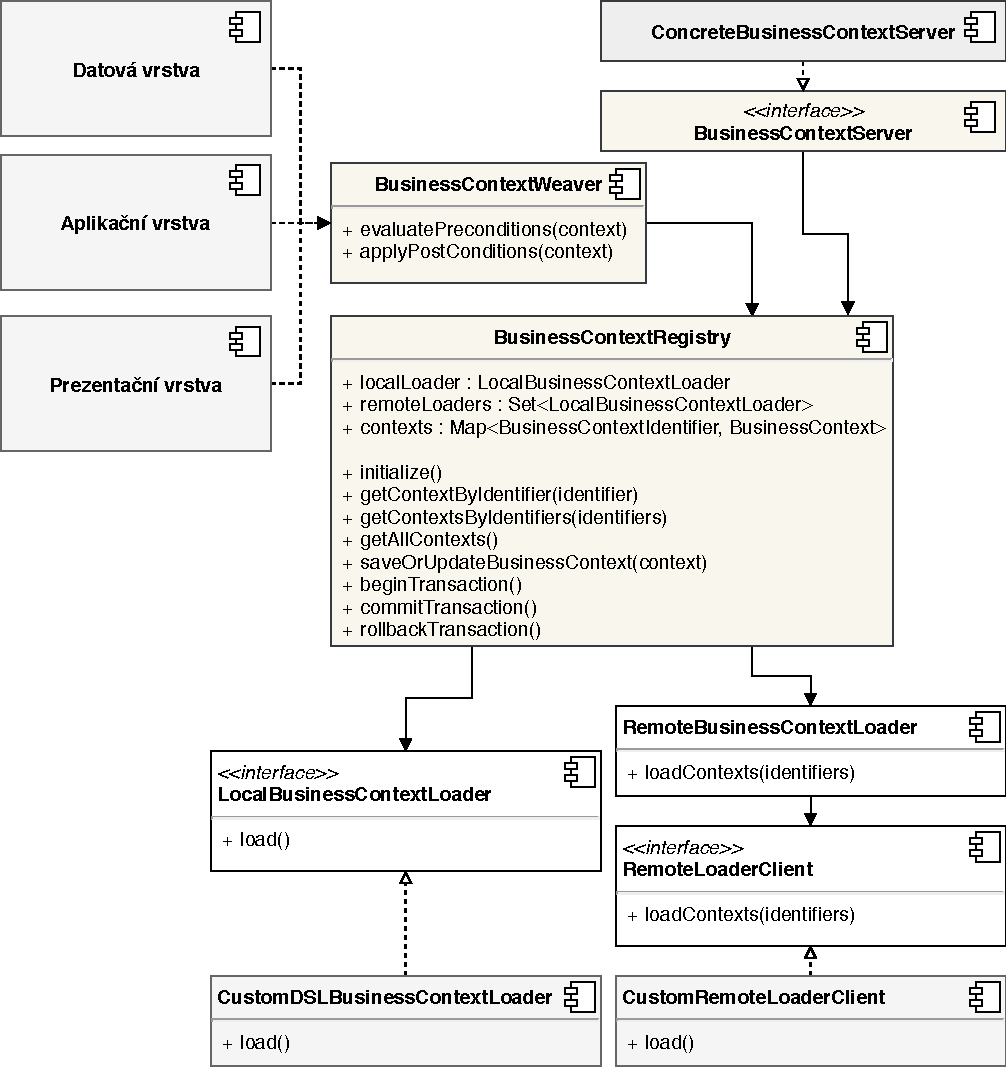
\includegraphics[keepaspectratio=true, width=\linewidth]{figures/business-context-registry.pdf}
    \caption{Architektura navrženého frameworku}
    \label{fig:business-context-registry}
\end{figure}

Základem frameworku je komponenta \code{BusinessContextRegistry}, tedy registr
byznysových kontextů, který je zodpovědný za inicializaci a uchovávání byznysových kontextů.
Načítání kontextů lze rozdělit na lokální a vzdálené. Při načítání lokálně dostupných kontextů
je potřeba získat \gls{DSL} kontextu ze souboru či databáze a převést ho do metamodelu.
K tomu bude využito rozhraní \code{LocalBusinessContextLoader}. Implementace rozhraní může být libovolná
a záviset na použitém \gls{DSL} či místu uložení pravidel. Naopak při načítání vzdálených
kontextů je potřeba vyžádat kontexty od vzdálené služby. O to se postará třída \code{RemoteBusinessContextLoader},
která požadované kontexty zorganizuje podle prefixu a poté pomocí rozhraní \code{RemoteLoaderClient} načte
pravidla od jednotlivých služeb. Implementace rozhraní \code{RemoteLoaderClient} bude záviset na použité
technologii a zajistí síťovou komunikaci a převod do a z formátu pro síťový přenos.
Aby mohl framework poskytovat lokální byznysové kontexty dané služby ke stažení, musí zastřešit
i serverovou funkcionalitu. K tomu slouží rozhraní \code{BusinessContextServer}. To bude využívat
\code{BusinessContextRegistry}, ze kterého načte byznysové kontexty, které si vyžádá \code{RemoteLoaderClient}.
Implementace serveru bude opět závislá na konkrétní technologii.
Nakonec bude framework obsahovat sadu aspect weaverů, které umožní weaving byznysových pravidel do
jednotlivých vrstev systému. Pro účely této práce bude framework poskytovat weavery pro využití v
aplikační vrstvě pro weaving preconditions a post-conditions do byznysových operací.
Architektura je zachycena na obrázku~\ref{fig:business-context-registry}.

\subsection{Service discovery}

% TODO: tohle možné nezmiňovat v samostatné kapitole, ale jen to zmínit při procesu načítání
Aby framework mohl distribuovat byznysové kontexty mezi službami, musí služba vyžadující kontext
znát adresu služby, od které ho vyžaduje. Adresy služeb mohou podléhat různým konfiguracím,
které se mohou lišit systém od systému. Framework proto nesmí být závislý na způsobu,
jakým se adresování služeb provádí. Nejlepším řešením je přenechat na uživateli frameworku, aby sám
získal a předal adresy služeb ve chvíli, kdy je framework potřebuje \textendash\xspace tedy
ve chvíli, kdy je potřeba načíst lokálně nedostupné kontexty.

\section{Shrnutí}

V této kapitole byl popsán návrh frameworku pro centrální správu a automatickou distribuci
byznysových pravidel v \gls{SOA} na základě přístupu \gls{ADDA}. Nejprve byla formalizována
doména byznysových pravidel v \gls{SOA} do názvosloví \gls{AOP}. Dále byla diskutována podobu byznysových pravidel,
jejich logických výrazů a jakým způsobem je lze zachytit v metamodelu a v \gls{DSL}.
Kapitola dále popisuje organizaci kontextů a procesy, kterými budou distribuovány a spravovány.
Nakonec byla shrnuta architektura frameworku.

%\usepackage[T1]{fontenc}
%\usepackage[utf8]{inputenc}

%!TEX ROOT=../diploma-thesis.tex

\chapter{Implementace prototypů knihoven frameworku}\label{ch:implementace}

%\goal{Uveden\'{\i} kapitoly a nast\'{\i}něn\'{\i} obsahu}
Součást\'{\i} zadán\'{\i} této práce je implementace prototypů
knihoven frameworku navrženého v kapitole~\ref{ch:navrh}
pro tři rozd\'{\i}lné platformy, z nichž jedna mus\'{\i} b\'yt \textit{Java}.
Tato kapitola popisuje výběr plaforem a konkrétní implementace
knihoven pro tyto platformy. Jelikož jednotlivé implementace
vycházejí ze stejného návrhu, kompletní implementace
je popsána pouze pro platformu Java. Ostatní implementace jsou
shrnuty komparativní metodou. Součástí kapitoly je i stručný popis
použitých technologií.

\section{V\'yběr použit\'ych platforem}

%\goal{Jaké jsme vybrali dalš\'{\i} platformy a proč}
Mimo jazyk Java, kter\'y byl určen zadán\'{\i}m, byla pro
implementaci vybrána platforma jazyka \textit{Python} a platforma \textit{Node.js},
která slouž\'{\i} jako běhové prostřed\'{\i} pro jazyk \textit{JavaScript}.
V\'yběr byl proveden na základě aktuáln\'{\i}ch trendů ve světě softwarového
inžen\'yrstv\'{\i}~\cite{githut}\cite{octoverse}\cite{stackoverflowsurvey}.
Tyto jazyky se v posledních letech stabilně umísťují na prvních příčkách
nejpopulárnějš\'{\i}ch programovacích jazyků pro obecné použit\'{\i}.

\section{Sd\'{\i}len\'{\i} byznys kontextů mezi službami}

%\goal{Formát pro přenos pravidel po s\'{\i}ti a jeho v\'yhody}
Pro sd\'{\i}lení byznysových kontextů a jejich pravidel
mezi jednotliv\'ymi službami je využita s\'{\i}ťová komunikace.
Ta musí probíhat ve formátu nezávislém na platformě, ideálně s vysokou
efektivitou přenosu. Návrh frameworku je však nezávislý na použité technologii.

\subsection{Protocol Buffers}

%\goal{Proč jsme použili Protobuf}
Pro prototypy knihoven byl pro přenos byznysových kontextů zvolen open-source formát
\textit{Protocol Buffers}\footnote{https://developers.google.com/protocol-buffers/}\cite{varda2008protocol}
vyvinut\'y společnost\'{\i} Google\footnote{https://www.google.com/}.
Ten umožňuje explicitně definovat a vynucovat schéma dat,
která jsou přenášena po s\'{\i}ti, bez vazby na konkrétn\'{\i} programovac\'{\i}
jazyk. Zároveň poskytuje obslužné knihovny pro vybrané platformy.
D\'{\i}ky binárn\'{\i} reprezentaci dat je v přenosu velmi efektivn\'{\i},
oproti formátům jako je \gls{JSON} nebo \gls{XML}~\cite{maeda2012performance}.
Na rozdíl od protokolů \textit{Apache Thrift}\footnote{https://thrift.apache.org/}
a \textit{Apache Avro}\footnote{https://avro.apache.org/}, které poskytuj\'{\i}
velmi srovnatelnou funkcionalitu, má zvolený protokol kvalitnějš\'{\i} a lépe
srozumitelnou dokumentaci.

\lstinputlisting[
caption={Část definice schématu zpráv byznys kontextů ve formátu Protocol Buffers},
label={lst:protobuf-example},
language=protobuf2,
style=protobuf,
%frame=single,
%float,
%floatplacement=H
]{code/protobuffer_example.proto}

Zdrojov\'y kód~\ref{lst:protobuf-example} znázorňuje zápis schématu
síťových zpráv pro distribucu byznys kontexty ve formátu Protobuffer.
Schéma zpráv pro v\'yměnu kontextů dodržuje strukturu metamodelu navrženého
v sekci~\ref{sec:metamodel}.

\begin{description}
    \item [ExpressionMessage] obsahuje jméno, atributy a argumenty \code{Expression}
    \item [ExpressionPropertyMessage] je enumerace obsahuj\'{\i}c\'{\i} typy atributu \code{Expression}
    \item [PreconditionMessage] obsahuje název a podm\'{\i}nku precondition pravidla
    \item [PostConditionMessage] obsahuje název, typ, název odkazovaného pole a podm\'{\i}nku post-condition pravidla
    \item [PostConditionTypeMessage] je enumerace obsahuj\'{\i}c\'{\i} typy post-condition pravidla
    \item [BusinessContextMessage] obsahuje identifikátor, seznam rožš\'{\i}řen\'ych kontextů, seznam preconditions a post-conditions byznys kontextu
    \item [BusinessContextsMessage] obaluje v\'{\i}ce byznys kontextů
\end{description}

\subsection{gRPC}

%\goal{Proč jsme použili gRPC}
Síťovou komunikaci potřebnou pro distribuci byznysových kontextů realizuje
open-source framework gRPC\footnote{https://grpc.io/}, kter\'y stav\'{\i}
na technologii Protocol Buffers. Tento framework poskytuje v\'yvojáři
možnost definovat detailn\'{\i} schéma komunikace pomoc\'{\i} protokolu \textit{\gls{RPC}}.
Zdrojov\'y kód~\ref{lst:grpc-example} znázorňuje zápis serveru,
kter\'y umožňuje volat metody \code{FetchContexts},
\code{FetchAllContexts} a \code{UpdateOrSaveContext}.

\lstinputlisting[
caption={Definice služby pro komunikaci byznys kontextů pro gRPC},
label={lst:grpc-example},
language=protobuf2,
style=protobuf,
%frame=single,
%float,
%floatplacement=H
]
{code/grpc_example.proto}

\paragraph{FetchContexts()} je procedura, která umožňuje klientovi
z\'{\i}skat kontexty, jejichž identifikátory zašle jako argument
typu \code{BusinessContextRequestMessage}.
V odpovědi pak obdrž\'{\i} dotazované kontexty a nebo chybovou hlášku,
pokud kontexty s dan\'ymi identifikátory nemá server k dispozici.

\paragraph{FetchAllContexts()} dovoluje klientovi z\'{\i}skat všechny
dostupné kontexty serveru. Tato metoda je využ\'{\i}vána pro administraci
kontextů, kdy je potřeba z\'{\i}skat všechny kontexty všech služeb, aby
nad nimi mohly prob\'{\i}hat úpravy a anal\'yzy.

\paragraph{UpdateOrSaveContext()} slouž\'{\i} pro uložen\'{\i} nového či
editovaného pravidla, které je zasláno v serializované podobě
jako jedin\'y argument typu \code{BusinessContextUpdateRequestMessage}.
Tato procedura musí být volána pouze pokud byla spuštěna transakce.

\paragraph{BeginTransaction()} spouští transakci, při které může proběhnout
změna nebo uložení nového byznysového kontextu.

\paragraph{CommitTransaction()} dokončuje transakci, která byla spuštěna pomocí \code{BeginTransaction()},
a uloží všechny změny byznysových kontextů.

\paragraph{RollbackTransaction()} zruší transakci, která byla spuštěna pomocí \code{BeginTransaction()}
a neuloží žádnou z provedených změn.

\section{Doménově specifick\'y jazyk pro popis byznys kontextů}\label{sec:dsl-impl}

%\goal{Popsat proč a jak jsme tvořili DSL}
Ačkoliv nen\'{\i} specifikace a implementace \gls{DSL} pro popis byznysových kontextů
úkolem této práce, pro ověřen\'{\i} konceptu je nutné nadefinovat alespoň jeho zjednodušenou
verzi a implementovat část knihovny, která bude umět jazyk zpracovat a sestavit metamodel popsaného
kontextu. Tento jazyk však bude možno v produkční verzi knihovny nahradit komplexnejším.

%\goal{Důvody pro v\'yběr XML}
Pro popis kontextů byl zvolen univerzáln\'{\i} formát Extensible
Markup Language (\gls{XML}) doplněný o definici schematu dat
pomocí \textit{XML Schema Definition}.
D\'{\i}ky formálně definovanému schématu lze popis byznys kontextu
automaticky validovat a vyvarovat se tak př\'{\i}padn\'ych chyb.

%\goal{Popis formátu}
Ve zdrojovém kódu~\ref{lst:business-context-xml} je znázorněn
př\'{\i}klad zápisu jednoduchého byznys kontextu s jednou precondition.
Samotn\'y zápis byznys kontextu je obsažen v kořenovém elementu
\code{<businessContext>} a jeho název je popsán atributy
\code{prefix} a \code{name}. Identifikátory rozš\'{\i}řených kontextů jsou
vypsány v entitě \code{<includedContexts>}. Preconditions jsou
definovány uvnitř entity \code{<preconditions>} a podobně
jsou definovány \code{<postconditions>}. Obsažená data odpov\'{\i}daj\'{\i}
navrženému metamodelu byznysového kontextu v sekci~\ref{sec:metamodel}.
Pro zápis podm\'{\i}nek jednotliv\'ych preconditions a post-conditions byl zvolen
opis derivačního stromu. Toto rozhodnut\'{\i} vycház\'{\i} z předpokladu,
že lze vzhledem k povaze prototypu relaxovat podm\'{\i}nku
na čitelnost zápisu pravidel ve prospěch jednodušš\'{\i}ho zpracován\'{\i}.

\lstinputlisting[
caption={Př\'{\i}klad zápisu byznys kontextu v jazyce \gls{XML}},
label={lst:business-context-xml},
language=XML,
%frame=single,
%float,
%floatplacement=H
]
{code/business_context.xml}

\section{Knihovna pro platformu Java}

Knihovna pro platformu Java se skládá ze čtyř modulů, které zajišťují
její funkcionalitu:

\begin{itemize}
    \item \code{business-context} obsahuje jádro knihovny
    \item \code{business-context-aspectj} poskytuje integraci s nástrojem AspectJ
    \item \code{business-context-grpc} přináší klienta a server pro distribuci byznysových pravidel pomocí frameworku gRPC
    \item \code{business-context-xml} obsahuje třídy pro čtení a zápis byznysových kontextů do \gls{XML}
\end{itemize}

Pro správu závislost\'{\i} a automatickou kompilaci a sestavován\'{\i}
všech těchto modulů byl zvolen projekt \textit{Maven}\footnote{https://maven.apache.org/}.
Tento nástroj umožňuje v\'yvojáři komfortně a centrálně spravovat závislosti jeho projektu včetně
detailn\'{\i}ho popisu jejich verze. Dále také umožňuje specifikovat a rozšiřovat kompilaci projektu.

\subsection{Jádro knihovny}

% Jádro knihovny
Jádro knihovny obsahuje metamodel a registr byznysových kontextů, weaver byznysových pravidel
a logické výrazy pravidel. Registr kontextů implementuje třída \code{BusinessContextRegistry},
která kromě funkcí popsaných v sekci~\ref{sec:registry-design} umožňuje snadnou konfiguraci
stahování vzdálených byznysových kontextů a načítání lokálních kontextů z \gls{DSL}.
Není závislá na konkrétních technologiích použitých pro síťovou komunikaci ani
na použitém \gls{DSL}.

% popis expressions
Logické výrazy byznysových pravidel jsou implementovány samostatnými třídami, které rozšiřují
jednotné rozhraní \code{Expression}. Toto rozhraní podporuje návrhový vzor Interpreter, který umožňuje
vyhodnocení výrazů, jak bylo popsáno v sekci~\ref{sec:expressions-design}. Zároveň je tím usnadněno
rozšíření knihovny o nové výrazy. Toto rozhraní navíc poskytuje metody, které usnadňují serializaci
výrazů.

\subsection{Weaving}

% popis weaveru
Weaver byznysových pravidel musí být schopen extrahovat informace o kontextu probíhající byznysové
operace, aby mohl správně zvolit příslušný byznysový kontext. V knihovne pro jazyk Java
byla pro tento účel zvolena anotace \code{BusinessOperation}, která umožňuje uživateli
knihovny označit metodu vykonávající byznysovou operaci. Parametry této metody mohou být
označeny anotací \code{BusinessContextParameter}. Weaver takto oanotované parametry vloží
jako proměnné do operačního kontextu a podmínky byznysových pravidel se na ně mohou odkazovat.
Ukázka použití těchto anotací je ve zdrojovém kódu~\ref{lst:business-operation-aspectj}.
Pomocí knihovny AspectJ\footnote{https://www.eclipse.org/aspectj/}, která poskytuje sadu nástrojů pro použití principů \gls{AOP},
je pak weaver pravidel volán ve chvíli, kdy je vykonávána anotovaná byznysová metoda.

\lstinputlisting[
caption={Označen\'{\i} operačn\'{\i}ho kontextu a jeho parametrů pomoc\'{\i} anotac\'{\i} Java knihovny},
label={lst:business-operation-aspectj},
language=Java,
%frame=single,
%float,
%floatplacement=H
]
{code/business_operation_aspectj.java}

\subsection{Serializace a deserializace XML}

% DSL XML
Pro serializaci a deserializici \gls{DSL} byznysových kontextů byly implementovány třídy
\code{BusinessContextXmlWriter} a \code{BusinessContextXmlLoader}. Ty využívají knihovnu
JDOM~2\footnote{http://www.jdom.org/}, která poskytuje
kompletn\'{\i} sadu nástroju pro čten\'{\i} a zápis \gls{XML} dokumentů.
Implementuje specifikaci \textit{Document Object Model}
pomoc\'{\i} které lze automaticky sestavovat a č\'{\i}st \gls{XML} dokumenty.

\subsection{Distribuce byznysových pravidel}

K distribuci byznysových pravidel mezi službami byly implementovány třídy
\code{GrpcBusinessContextServer} a \code{GrpcBusinessContextClient}.
Framework gRPC poskytuje knihovnu pro jazyk Java, která vygeneruje \textit{Stub}
zapouzdřující veškerou síťovou komunikaci. Obsluha komunikace tak vyžaduje pouze
sepsání obslužného kódu, který převede byznysové kontexty z metamodelu a zpět.
Obě třídy navíc obsahují metody pro snadnou konfiguraci sítových adres.

\section{Knihovna pro platformu Python}

Knihovna pro platformu Python využ\'{\i}vá verzi jazyka 3.6.
Skládá se ze tří částí: \code{business\_context} obsahuje jádro knihovny,
\code{business\_context\_grpc} umožňuje síťovou komunikaci pomocí frameworku
gRPC a \code{business\_context\_xml} poskytuje nástroje pro zápis a čtení kontextů z \gls{XML}.
Pomoc\'{\i} nástroje \textit{pip}\footnote{https://pip.pypa.io/en/stable/}
lze jednotlivé části knihovny nainstalovat a využ\'{\i}vat jako samostatné
Python moduly. Implementace odpov\'{\i}dá navržené specifikaci.

\subsection{Srovnán\'{\i} s knihovnou pro platformu Java}

\paragraph{Weaving} Největš\'{\i}m rozd\'{\i}lem oproti knihovně pro
jazyk Java je implementace weavingu byznys kontextů.
Jazyk Python totiž d\'{\i}ky své dynamické povaze a vestavěnému
systému dekorátorů umožňuje aplikovat principy aspektově orientovaného
programován\'{\i} bez potřeby dodatečn\'ych knihoven či technologi\'{\i}.
Zdrojov\'y kód~\ref{lst:python-weaving-example} znázorňuje
definici a použit\'{\i} dekorátoru \code{business\textunderscore operation}.
Dekorátoru je potřeba předat samotn\'y weaver, narozd\'{\i}l
od implementace v Javě, kdy se o předán\'{\i} weaveru postará dependency
injection container.

\lstinputlisting[
caption={Př\'{\i}klad použit\'{\i} dekorátorů pro weaving v jazyce Python},
label={lst:python-weaving-example},
language=Python,
%frame=single,
%float,
%floatplacement=H
]
{code/python_weaving.py}

\paragraph{Jména tříd a metod} Jazyk Python využívá jiné jmenné konvence
a jinak člení kód do jednotlivých souborů. Aby byly tyto konvence zachovány,
třídy knihovny a názvy jejich metod se liší od těch v jazyce Java.

\subsection{Použité technologie}

Jazyk Python poskytuje na rozdíl od jazyka Java téměř všechny nástroje, které byly pro implementaci
prototypu knihovny potřeba. Jedinou výjimkou byl modul pro obsluhu frameworku gRPC.
Ze standardní knihovny jazyka byly využity moduly \code{typing} pro statické typování,
\code{re} pro regulární výrazy, \code{enum} pro implementaci výčtových hodnot, \code{copy} pro
kopírování objektů a \code{xml} pro práci s XML dokumenty.

\section{Knihovna pro platformu Node.js}

Knihovna pro platformu \textit{Node.js} byla implementována
v jazyce JavaScript, konkrétně ve verzi \textit{ECMAScript 6.0}.
Implementace odpov\'{\i}dá specifikaci návrhu, umožňuje
instalaci pomoc\'{\i} bal\'{\i}čkovac\'{\i}ho nástroje a snadnou
integraci do kódu v\'ysledné služby. Stejně jako knihovna
pro jazyk Python se skládá ze tří modulů: \code{business-context} obsahuje
jádro knihovny, \code{business-context-grpc} poskytuje server a klienta pro distribuci
byznysových kontextů po síti pomocí frameworku gRPC a \code{business-context-xml} umožňuje
serializaci a deserializaci z XML.

\subsection{Srovnán\'{\i} s knihovnou pro platformu Java}

\paragraph{Weaving} Podobně jako v knihovně pro jazyk Python,
i v knihovně pro Node.js byl oproti knihovně pro jazyk Java
největš\'{\i} rozd\'{\i}l v implementaci weavingu. Platforma Node.js
totiž nedisponuje žádnou kvalitn\'{\i} knihovnou, která by ulehčila
využit\'{\i} konceptů aspektově orientovaného programován\'{\i}.
Jazyk JavaScript však podobně jako jazyk Python umožňuje využ\'{\i}t
princip dekorátoru funkce. Ukázka takového dekorátoru je ve zdrojovém
kódu~\ref{lst:nodejs-weaving}. Funkce \code{register()} obsahuje logiku pro registraci uživatele,
která může obsahovat např\'{\i}klad uložen\'{\i} entity do databáze a odeslán\'{\i}
registračn\'{\i}ho emailu. Při exportován\'{\i} funkce z Node.js modulu
je využita funkce \code{wrapCall()}, která má za úkol dekorovat
předanou funkci \code{func}, před jej\'{\i}m zavolán\'{\i} vyhodnotit
preconditions a po zavolán\'{\i} aplikovat post-conditions.
D\'{\i}ky tomu bude každ\'y kód, kter\'y využije modul definuj\'{\i}c\'{\i} funkci
pro registraci uživatele, pracovat s dekorovanou funkc\'{\i}.

\paragraph{Využit\'{\i} gRPC} Narozd\'{\i}l od implementac\'{\i} knihovny
v jazyc\'{\i}ch Java a Python um\'{\i} knihovna obsluhuj\'{\i}c\'{\i} gRPC
fungovat i bez předgenerovaného kódu. To poněkud usnadnilo
práci při serializaci byznys kontextů do přenosového formátu
i při deserializaci a ukládán\'{\i} kontextů do paměti. Úspora
kódu je ale na úkor typové kontroly a tak může b\'yt kód náchylnějš\'{\i}
na lidskou chybu.

\lstinputlisting[
caption={Př\'{\i}klad dekorace funkce v JavaScriptu pro aplikaci weavingu},
label={lst:nodejs-weaving},
language=JavaScript,
%frame=single,
%float,
%floatplacement=H
]
{code/nodejs_weaving.js}

\subsection{Použité technologie}

%\goal{Použité technologie pro v\'yvoj knihovny}
Podobně jako byl použit nástroj Maven pro knihovnu v jazyce Java byl
využit bal\'{\i}čkovac\'{\i} nástroj \textit{NPM}, kter\'y je předinstalován
v běhovém prostřed\'{\i} \textit{Node.js}. Tento nástroj ale nedisponuje
př\'{\i}liš silnou podporou pro správu automatick\'ych sestaven\'{\i} knihovny
a v základn\'{\i}m nastaven\'{\i} nen\'{\i} ani př\'{\i}liš efektivn\'{\i} pro správu závislost\'{\i}.
Proto bylo nutné využ\'{\i}t dodatečné knihovny, jmenovitě
\textit{Yarn}\footnote{https://yarnpkg.com/en/}, \textit{Babel}\footnote{https://babeljs.io/} a
\textit{Rimraf}\footnote{https://github.com/isaacs/rimraf}.

\section{Systém pro centráln\'{\i} správu byznys pravidel}\label{sec:central-administration}

Součástí této práce je i implementace nástroje, který umožní centrální správu byznysových
pravidel
\subsection{Popis implementace}

Systém pro centrální správu ...

Pro komfortn\'{\i} obsluhu centráln\'{\i} administrace bylo naprogramováno
uživatelské rozhran\'{\i} pomoc\'{\i} technologi\'{\i} Hypertext Markup Language
(HTML) a Cascading Style Sheets (\gls{CSS}).
Detail byznysového kontextu v uživatelském rozhran\'{\i} je zobrazen
na sn\'{\i}mku~\ref{fig:screenshot-context-detail} a formulář pro úpravu kontextu
na sn\'{\i}mku~\ref{fig:screenshot-context-edit}.

\todo{
\begin{itemize}
    \item Uživatelské rozhran\'{\i} v HTML + CSS
    \item Jak jsme použili Spring Boot a jeho MVC k nastaven\'{\i} základn\'{\i} webové aplikace
    \item Dependency Injection Container
    \item Využit\'{\i} knihovny pro platformu Java
\end{itemize}
}

\subsection{Detekce a prevence potenciáln\'{\i}ch problémů}

%\goal{Problémy způsobené rozšiřován\'{\i}m kontextů}
Sekce~\ref{sec:context-inheritance} identifikuje problémy, které
mohou nastat při úpravě nebo vytvářen\'{\i} nového byznysového kontextu.
Kromě syntaktick\'ych chyb, které jsou detekovány automaticky pomoc\'{\i} definovaného schematu,
je potřeba detekovat následující sémantické chyby, které mohou b\'yt způsobeny rozšiřován\'{\i}m kontextů.
\begin{enumerate}[label=\alph*)]
    \item Neunikátní identifikátory byznysových pravidel
    \item Závislosti na neexistuj\'{\i}c\'{\i}ch kontextech
    \item Cyklus v grafu závislost\'{\i} kontextů
\end{enumerate}

%\goal{Chápán\'{\i} kontextů jako grafu}
Unikátnost byznysových pravidel lze zajistit postupným ukládáním jejich identifikátorů
do vhodné datové struktury a kontrolovat, zda již nejsou ve struktuře obsaženy. Vhodnou
strukturou je například \code{Set}~\cite{hopcroft1983data}.
Kontexty a jejich vzájemné závislosti lze vn\'{\i}mat jako
orientovan\'y graf, kde uzel grafu reprezentuje kontext
a orientovaná hrana reprezentuje závislost mezi kontexty.
Směr závislosti lze pro tento účel zvolit libovolně.
Pro detekci závislosti na neexistuj\'{\i}c\'{\i}ch kontextech je nejprve
sestaven seznam existuj\'{\i}c\'{\i}ch kontextů a následně jsou navštíveny
jednotlivé hrany grafu kontextů a je ověřeno, zda existuj\'{\i} oba kontexty
nálež\'{\i}c\'{\i} dané hraně. Při zvolen\'{\i} vhodn\'ych datov\'ych struktur
lze dosáhnout lineárn\'{\i} složitosti v závislosti na počtu hran grafu.
Pro detekci cyklů v grafu závislosti pravidel popsanou v sekci~\ref{sec:context-inheritance} byl
zvolen Tarjanův algoritmus~\cite{tarjan1971depth}. Ten umožňuje detekci souvisl\'ych
komponent a má lineárn\'{\i} složitost závislou na součtu počtu hran a
počtu uzlů grafu. V př\'{\i}padě, že zápis nového či upraveného kontextu obsahuje syntaktické
nebo sémantické chyby, administrace nedovol\'{\i} uživateli změnu provést a vyp\'{\i}še informativn\'{\i}
chybovou hlášku.

\section{Shrnutí}

%\goal{Dosáhli jsme vytyčen\'ych c\'{\i}lů implementace}
Na základě navrženého frameworku byly implementovány prototypy
knihoven pro platformy jazyka Java, jazyka Python a
Node.js. Knihovny umožňuj\'{\i} centráln\'{\i} správu a automatickou distribuci a integraci
byznysov\'ych kontextů, včetně vyhodnocován\'{\i} jejich pravidel, za
použit\'{\i} aspektově orientovaného př\'{\i}stupu.
V rámci této kapitoly byl specifikován \gls{DSL}, kter\'ym lze popsat
byznys kontext nezávisle na platformě.
Implementované protoypy knihoven lze využ\'{\i}t k implementaci služeb a k sestaven\'{\i}
funkčn\'{\i}ho systému, jak je popisáno v následuj\'{\i}c\'{\i} kapitole.

%\goal{Hostován\'{\i} na GitHubu + licence}
Vešker\'y kód implementace je hostován v centráln\'{\i}m repozitáři
ve službě GitHub\footnote{https://github.com/klimesf/diploma-thesis}
a je zpř\'{\i}stupněn pod open-source licenc\'{\i} \gls{MIT}~\cite{mitlicense}.
Knihovny pro jednotlivé platformy tedy lze libovolně
využ\'{\i}vat, modifikovat a š\'{\i}řit.

%\usepackage[T1]{fontenc}
%\usepackage[utf8]{inputenc}

%!TEX ROOT=../diploma-thesis.tex

\chapter{Testování a validace frameworku}\label{ch:testovani}

Tato kapitola popisuje, jak\'y způsobem bylo provedeno
tetování naprogramovan\'ych knihoven pomoc\'{\i}
jednotkov\'ych a integračn\'{\i}ch testů.
Kapitola se dále věnuje popisu ukázkového systému, na kterém
byla demonstrována správná funkčnost navrženého frameworku
a provedena analýza vlivu jeho nasazení na duplikaci
byznysových pravidel.

\section{Testován\'{\i} prototypů knihoven}

Prototypy knihoven, jejichž implementaci je popsána v kapitole~\ref{ch:implementace},
byly důkladně otestovány pomoc\'{\i} sady jednotkov\'ych a integračn\'{\i}ch testů~\cite{luo2001software}
a t\'{\i}m byla otestována jejich správná funkcionalita. Způsob
testován\'{\i} knihoven je popsán zvlášť pro každou platformu.

V rámci konceptu \textit{continous integration} (\gls{CI})~\cite{fowler2006continuous}
byl kód po celou dobu v\'yvoje verzován systémem Git\footnote{\url{https://git-scm.com/}},
zas\'{\i}lán do centráln\'{\i}ho repozitáře a s pomoc\'{\i}
nástroje Travis \gls{CI}\footnote{\url{https://travis-ci.org/}}
bylo automaticky spouštěno jeho sestaven\'{\i} a otestován\'{\i}.
Systém zároveň okamžitě informoval v\'yvojáře o v\'ysledc\'{\i}ch.
To umožnilo v krátkém časovém horizontu identifikovat konkrétn\'{\i} změny
v kódu, které do programu vnesly chybu. T\'{\i}m byla sn\'{\i}žena
pravděpodobnost regrese a dlouhodobě se zv\'yšila celková kvalita kódu.

\subsection{Jednotkové testy}

% TODO: popsat co to je

\subsection{Integrační testy}

% TODO: popsat co to je

\subsection{Testovací scénáře}

Každá z knihoven byla testována stejnou sadou testovacích scénářů, které jsou shrnuty
v tabulce~\ref{tbl:test-cases}. K implementaci a vyhodnocení testů byly pro jednotlivé
knihovny použity různé technologie, které jsou popsány v následujícím textu.

\begin{table}
    \centering
    \begin{tabular*}{\textwidth}{ l l }
        \hline
        \textbf{\#} & \textbf{Popis} \\ \hline \hline
        \textbf{TC01} & \makecell[l]{Pouze identifikátor byznysového kontextu obsahující alfanumerický prefix \\ a název je validní} \\ \hline
        \textbf{TC02} & \makecell[l]{Precondition weaver zkontroluje všechny preconditions vztahující se \\ k aktuálnímu kontextu} \\ \hline
        \textbf{TC03} & \makecell[l]{Precondition weaver nevyhodí výjimku, pokud jsou všechny preconditions \\ splněny} \\ \hline
        \textbf{TC04} & \makecell[l]{Precondition weaver vyhodí výjimku, pokud alespoň jedna precondition \\ není splněna} \\ \hline
        \textbf{TC05} & \makecell[l]{Post-condition weaver aplikuje všechny post-conditions vztahující se \\ k aktuálnímu kontextu} \\ \hline
        \textbf{TC06} & Post-condition weaver správně filtruje atribut objektu \\ \hline
        \textbf{TC07} & Post-condition weaver správně filtruje pole hodnot \\ \hline
        \textbf{TC08} & Post-condition weaver správně filtruje atributy objektů v poli \\ \hline
        \textbf{TC09} & Logický výraz \code{And} odpovídá logické konjunkci \\ \hline
        \textbf{TC10} & Logický výraz \code{Equals} odpovídá logické ekvivalenci \\ \hline
        \textbf{TC11} & Logický výraz \code{Negate} odpovídá logické negaci \\ \hline
        \textbf{TC12} & Logický výraz \code{Or} odpovídá logické disjunkci \\ \hline
        \textbf{TC13} & \makecell[l]{Výraz \code{Constant} správně doplňuje do pravidla konstantu} \\ \hline
        \textbf{TC14} & \makecell[l]{Výraz \code{FunctionCall} správně volá externí funkci} \\ \hline
        \textbf{TC15} & \makecell[l]{Výraz \code{IsNotNull} správně kontroluje, zda v jeho argumentu není prázdný výraz} \\ \hline
        \textbf{TC16} & \makecell[l]{Výraz \code{IsNotBlank} správně kontroluje, zda v jeho argumentu není prázdný \\ řetězec} \\ \hline
        \textbf{TC17} & \makecell[l]{Výraz \code{ObjectPropertyReference} správně vkládá do výrazu hodnotu atributu \\ objektu z kontextu} \\ \hline
        \textbf{TC18} & \makecell[l]{Výraz \code{VariableReference} správně vkládá do výrazu hodnotu proměnné \\ z kontextu} \\ \hline
        \textbf{TC19} & \makecell[l]{Byznysové kontexty jsou korektně inicializovány, jejich závislosti staženy \\ a spojeny} \\ \hline
        \textbf{TC20} & Byznysové kontexty jsou správně a kompletně přenášeny mezi službami \\ \hline
        \textbf{TC21} & Při dokončení transakce se správně uloží upravené i nové byznysové kontexty \\ \hline
        \textbf{TC21} & Při zrušení transakce se neuloží upravené ani nové byznysové kontexty \\ \hline
        \textbf{TC22} & Spouštění byznysových operací je pozastaveno při probíhající transakci \\ \hline
        \textbf{TC23} & Byznysové kontexty jsou správně deserializovány z \gls{XML} \\ \hline
        \textbf{TC24} & Byznysové kontexty jsou správně serializovány do \gls{XML} \\ \hline
        \hline
    \end{tabular*}
    \caption{Testovací scénáře prototypů knihoven}
    \label{tbl:test-cases}
\end{table}

\subsection{Platforma Java}

Prototyp knihovny pro platformu jazyka Java byl testován pomoc\'{\i}
nástroje JUnit\footnote{\url{https://junit.org/junit4/}}, kter\'y poskytuje veškerou potřebnou funkcionalitu pro
jednotkové i integračn\'{\i} testován\'{\i}. Všechny testy byly spouštěny automaticky
při sestavován\'{\i} knihovny pomoc\'{\i} nástroje Maven\footnote{\url{https://maven.apache.org/}}.

\lstinputlisting[
caption={Jednotkový test knihovny pro jazyk Java s využit\'{\i}m nástroje JUnit 4},
label={lst:java-testing},
language=Java,
%frame=single,
]
{code/test_example.java}

Ve zdrojovém kódu~\ref{lst:java-testing} je znázorněn jednotkov\'y test
tř\'{\i}dy \code{BusinessContextWeaver} odpovídající testovacímu scénáři \textit{TC06}, konkrétně
filtrování pole \code{email} objektu \code{user}. Anotace \code{@Test} metody \code{test()} znač\'{\i},
že metoda obsahuje \textit{test case} a framework JUnit zajist\'{\i}, že bude spuštěna
a vyhodnocena. Statické metody tř\'{\i}dy \code{Assert} ověř\'{\i}, zda uživateli zůstalo
vyplněno jméno, ale emailová adresa ne.

\subsection{Platforma Python}

Prototyp knihovny pro platformu jazyka Python byl testován pomoc\'{\i}
nástroje \code{unittest}\footnote{\url{https://docs.python.org/3/library/unittest.html}}, inspirovaného nástrojem
JUnit. Ačkoliv jméno obou nástrojů nasvědčuje, že slouž\'{\i} zejména pro jednotkové testy,
lze je plně využ\'{\i}t i pro integračn\'{\i} testy.

\lstinputlisting[
caption={Jednotkový test knihovny pro jazyk Python s využit\'{\i}m nástroje Unittest},
label={lst:python-testing},
language=Python,
%frame=single,
]
{code/test_example.py}

Ve zdrojovém kódu~\ref{lst:python-testing} je př\'{\i}klad jednotkového testu tř\'{\i}dy
\code{Identifier} se třemi metodami ověřuj\'{\i}c\'{\i}mi testovací scénář \textit{TC01}.
Funkce \code{test\_split()} ověřuje, zda konstruktor správně přij\'{\i}má dva argumenty,
kde prvn\'{\i} z nich je prefix identifikátoru a druh\'y je jméno identifikátoru.
Funkce \code{test\_single()} naopak ověřuje, zda kontruktor správně přij\'{\i}má jeden
argument a rozděl\'{\i} ho na prefix a jméno identifikátoru.
Nakonec funkce \code{test\_str()} ověřuje správnou funkcionalitu převeden\'{\i}
identifikátoru na textov\'y řetězec.

\subsection{Platforma Node.js}

Tendence ve světě modern\'{\i}ho JavaScriptu je vytvářet knihovny s co nejmenš\'{\i}m polem působnosti,
které jdou kombinovat do větš\'{\i}ho celku. Prototyp knihovny pro platformu Node.js byl proto testován pomoc\'{\i}
kombinace dvou nástrojů. Spouštěn\'{\i} testů obstarává knihovna \textit{Mocha}\footnote{\url{https://mochajs.org/}}, zat\'{\i}mco
ověřován\'{\i} a zápis testů ve stylu \textit{Behaviour Driven Development} poskytuje knihovna \textit{Chai}\footnote{\url{http://www.chaijs.com/}}.

\lstinputlisting[
caption={Jednotkový test knihovny pro platformu Node.js s využit\'{\i}m nástroje Mocha a Chai},
label={lst:nodejs-testing},
language=JavaScript,
%frame=single,
]
{code/test_example.js}

Zdrojov\'y kód~\ref{lst:nodejs-testing} znázorňuje použit\'{\i} testovacích knihoven k implementaci testovacího
scénáře \textit{TC15} ověřující funkcionalitu výrazu \code{IsNotNull}. Konkrétně je výraz nejprve zkonstruován s
konstantn\'{\i}m argumentem typu \code{boolean} s hodnotou \code{true} a je ověřeno, že v\'yraz se vyhodnot\'{\i}
jako \code{true}. Následně je zkonstruován v\'yraz, kterému je předán argument \code{null} a je ověřeno,
že v\'yraz se vyhodnot\'{\i} jako \code{false}.

\section{Ukázkový příklad: e-commerce systém}

Pro praktické testování a validaci navrženého frameworku bylo nutné vyzkoušet
jeho nasazen\'{\i} při v\'yvoji aplikace. Pro tento účel vznikl v
rámci této práce ukázkový příklad na fiktivn\'{\i}m
e-commerce systému využ\'{\i}vaj\'{\i}c\'{\i}m architekturu orientovanou na služby.
Na tomto př\'{\i}kladě je demonstrována schopnost frameworku poradit si s průřezov\'ymi
problémy v rámci \gls{SOA} a také jeho schopnost plnit požadavky identifikované v
sekci~\ref{sec:implementation-requirements}.

% TODO: motivace a účel systému

\subsection{Use-cases}

Pro ukázkov\'y systém bylo vymodelováno třináct př\'{\i}padů užit\'{\i}
(z anglického \textit{Use case} (\gls{UC})~\cite{bittner2002use}), jejich
přehled je v tabulce~\ref{tbl:use-cases}.

\begin{table}[h]
    \centering
    \begin{tabular*}{\textwidth}{ l l }
        \hline
        \textbf{\#} & \textbf{Use-case} \\
        \hline \hline
        \textbf{UC01} & Nepřihlášen\'y uživatel si může vytvořit zákaznick\'y účet \\
        \textbf{UC02} & Zákazn\'{\i}k může prohl\'{\i}žet produkty \\
        \textbf{UC03} & Zákazn\'{\i}k může vkládat produkty do koš\'{\i}ku \\
        \textbf{UC04} & Zákazn\'{\i}k může vytvořit objednávku \\
        \textbf{UC05} & Skladn\'{\i}k může do systému zadávat nové produkty \\
        \textbf{UC06} & Skladn\'{\i}k může upravovat u produktů stav skladov\'ych zásob \\
        \textbf{UC07} & Skladn\'{\i}k si může zobrazovat objednávky \\
        \textbf{UC08} & Skladn\'{\i}k může upravovat stav objednávek \\
        \textbf{UC09} & Administrátor si může prohl\'{\i}žet objednávky \\
        \textbf{UC10} & Administrátor může upravovat cenu produktů \\
        \textbf{UC11} & Administrátor může vytvářet uživatele (skladn\'{\i}ky) \\
        \textbf{UC12} & Administrátor může mazat uživatele (skladn\'{\i}ky i zákazn\'{\i}ky) \\
        \textbf{UC13} & Administrátor může vystavit fakturu \\
        \hline
    \end{tabular*}
    \caption{Případy použití ukázkového e-commerce systému}
    \label{tbl:use-cases}
\end{table}

\subsection{Model systému}

Na obrázku~\ref{fig:example-model} je diagram tř\'{\i}d reprezentuj\'{\i}c\'{\i}ch
kompletn\'{\i} doménov\'y model ukázkového systému.

\begin{itemize}
    \item \textbf{\code{UserRole}} reprezentuje uživatelskou roli v systému.
    \item \textbf{\code{User}} je entita odpov\'{\i}daj\'{\i}c\'{\i} uživateli, ať už zákazn\'{\i}kovi, či zaměstnanci.
    \item \textbf{\code{Product}} popisuje konkrétn\'{\i} produkt v nab\'{\i}dce společnosti a jeho nákupn\'{\i} a prodejn\'{\i} cenu.
    \item \textbf{\code{Order}} odpov\'{\i}dá objednávce, má vazbu na dodac\'{\i} a fakturačn\'{\i} adresu a také na položky objednávky.
    \item \textbf{\code{OrderItem}} reprezentuje položku objednávky a uchovává údaje o počtu objednan\'ych kusů produktu.
    \item \textbf{\code{Address}} je entita popisuj\'{\i}c\'{\i} dodac\'{\i} či fakturačn\'{\i} adresu.
\end{itemize}

\begin{figure}[t]
    \centering
    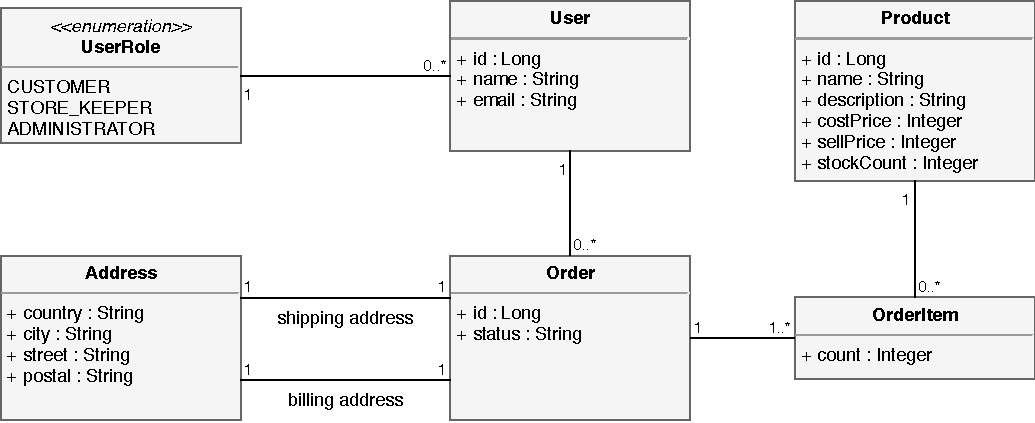
\includegraphics[keepaspectratio=true, width=0.9\linewidth]{figures/example-model.pdf}
    \caption{Doménový model ukázkového e-commerce systému}
    \label{fig:example-model}
\end{figure}

Tento model je využ\'{\i}ván v každé ze služeb. Nicméně, ne každá služba využije všechny jeho entity,
ale pouze jejich podmnožinu, kterou potřebuje ke svoj\'{\i} práci.

\subsection{Byznysová pravidla a kontexty}

V tabulce~\ref{tbl:business-rules} je v\'yčet všech dvaceti byznysov\'ych pravidel, která byla
vymodelována pro ukázkovou aplikaci. V tabulce kromě identifikátoru a popisu byznysového pravidla
vid\'{\i}me, na které užitné př\'{\i}pady se pravidlo aplikuje, a jak\'y je typ pravidla
(\textit{pre} pro precondition, \textit{post} pro post-condition).

\begin{table}
    \centering
    \begin{tabular}{ l l l r }
        \hline
        \textbf{\#} & \textbf{Use-cases} & \textbf{Pravidlo} & \textbf{Typ} \\ \hline \hline
        \textbf{BR01} & UC01 & Uživatel nesm\'{\i} b\'yt přihlášen\'y & pre \\ \hline
        \textbf{BR02} & UC02, UC03 & \makecell[l]{Uživatel nesm\'{\i} zobrazovat ani manipulovat \\ s produkty, které nejsou aktivn\'{\i}} & post \\ \hline
        \textbf{BR03} & UC02 až UC04 & \makecell[l]{Uživatel nesm\'{\i} u produktu vidět nákupn\'{\i} cenu, \\ pouze v\'yslednou cenu} & post \\ \hline
        \textbf{BR04} & UC04 & \makecell[l]{Zákazník mus\'{\i} řádně vyplnit doručovac\'{\i} \\ adresu (č.p., ulice, město, PSČ, stát)} & pre \\ \hline
        \textbf{BR05} & UC04, UC13 & \makecell[l]{Zákazník mus\'{\i} řádně vyplnit fakturačn\'{\i} \\ adresu (č.p., ulice, město, PSČ, stát)} & pre \\ \hline
        \textbf{BR06} & UC01, UC04, UC11 & Uživatel mus\'{\i} m\'{\i}t vyplněnou emailovou adresu & pre \\ \hline
        \textbf{BR07} & UC03 & Nákupní košík může obsahovat maximálně 10 položek & pre \\ \hline
        \textbf{BR08} & UC04 & \makecell[l]{Položky objednávky mus\'{\i} m\'{\i}t počet kusů menš\'{\i}, \\ než je aktuáln\'{\i} stav skladov\'ych zásob produktu} & pre \\ \hline
        \textbf{BR09} & UC04 & \makecell[l]{Stát mus\'{\i} b\'yt v seznamu zem\'{\i}, \\ do kter\'ych firma doručuje} & pre \\ \hline
        \textbf{BR10} & UC04 & Zákazn\'{\i}k mus\'{\i} b\'yt přihlášen & pre \\ \hline
        \textbf{BR11} & UC05 až UC08 & \makecell[l]{Skladn\'{\i}k mus\'{\i} b\'yt do systému přihlášen \\ a m\'{\i}t roli "Skladn\'{\i}k"} & pre \\ \hline
        \textbf{BR12} & UC02 & \makecell[l]{Skladn\'{\i}k u produktu nesm\'{\i} vidět nákupn\'{\i} cenu, \\ pouze v\'yslednou cenu} & post \\ \hline
        \textbf{BR13} & UC05 & Produkt mus\'{\i} m\'{\i}t jméno s délkou >5 & pre \\ \hline
        \textbf{BR14} & UC06 & Stav zásob produktů mus\'{\i} b\'yt č\'{\i}slo větš\'{\i} nebo rovno 0 & pre \\ \hline
        \textbf{BR15} & UC08 & \makecell[l]{Stav objednávky mus\'{\i} b\'yt pouze "přijato", \\ "expedováno" a "doručeno"} & pre \\ \hline
        \textbf{BR16} & UC09 až UC13 & \makecell[l]{Administrátor mus\'{\i} b\'yt do systému přihlášen \\ a m\'{\i}t roli "Administrátor"} & pre \\ \hline
        \textbf{BR17} & UC10 & \makecell[l]{V\'ysledná cena produktu mus\'{\i} b\'yt větš\'{\i} \\ než jeho nákupn\'{\i} cena} & pre \\ \hline
        \textbf{BR18} & UC11 & Skladn\'{\i}k mus\'{\i} m\'{\i}t jméno delš\'{\i} než 2 znaky & pre \\ \hline
        \textbf{BR19} & UC12 & Smazaný uživatel nesmí být administrátor & pre \\ \hline
        \hline
    \end{tabular}
    \caption{Byznysová pravidla ukázkového e-commerce systému}
    \label{tbl:business-rules}
\end{table}

Dále jsou v tabulce~\ref{tbl:business-contexts} vypsány všechny byznysové kontexty v ukázkové aplikaci.
Některé z nich jsou konkrétn\'{\i} a jsou namapovány na jeden nebo v\'{\i}ce \gls{UC},
jiné jsou abstraktn\'{\i} a slouž\'{\i} ostatn\'{\i} kontexty je rozšiřuj\'{\i}.
Prefixy byly vybrány na základě byznysové domény, ke které se kontext vzahuje, stajně jako
jsou podle domén děleny i jednotlivé služby systému.

\begin{table}
    \centering
    \begin{tabular*}{\textwidth}{ l c l }
        \hline
        \textbf{Identifikátor} & \textbf{Use-cases} & \textbf{Byznysová pravidla} \\ \hline \hline
        \textbf{auth.adminLoggedIn} & - & BR16 \\ \hline
        \textbf{auth.employeeLoggedIn} & - & BR11 \\ \hline
        \textbf{auth.userLoggedIn} & - & BR10 \\ \hline
        \textbf{billing.correctAddress} & - & BR05 \\ \hline
        \textbf{billing.createInvoice} & UC13 & BR05 \\ \hline
        \textbf{order.addToShippingCart} & UC03 & BR02, BR07, BR08, BR10 \\ \hline
        \textbf{order.changeStatus} & UC08 & \makecell[l]{BR04, BR05, BR06, BR08, BR09, BR11, \\ BR15} \\ \hline
        \textbf{order.create} & UC04 & \makecell[l]{BR03, BR04, BR05, BR06, BR07, BR08, \\ BR09, BR10, BR15} \\ \hline
        \textbf{order.listAll} & UC07, UC09 & BR11 \\ \hline
        \textbf{order.valid} & - & BR04, BR05, BR06, BR09, BR15 \\ \hline
        \textbf{product.changePrice} & UC10 & BR16, BR17 \\ \hline
        \textbf{product.changeStock} & UC06 & BR08, BR11, BR14 \\ \hline
        \textbf{product.create} & UC05 & BR10, BR11, BR13, BR14 \\ \hline
        \textbf{product.detail} & UC02 & BR02, BR03, BR10, BR12 \\ \hline
        \textbf{product.hidden} & - & BR02 \\ \hline
        \textbf{product.listAll} & UC02 & BR02, BR03, BR12 \\ \hline
        \textbf{shipping.correctAddress} & - & BR04, BR09 \\ \hline
        \textbf{user.createCustomer} & UC01 & BR01, BR06 \\ \hline
        \textbf{user.createEmployee} & UC11 & BR06, BR16, BR18 \\ \hline
        \textbf{user.delete} & UC12 & BR16, BR19 \\ \hline
        \textbf{user.validEmail} & - & BR06 \\ \hline
        \hline
    \end{tabular*}
    \caption{Byznysové kontexty ukázkového e-commerce systému}
    \label{tbl:business-contexts}
\end{table}

Na obrázku~\ref{fig:example-system-context-hirearchy} je vizualizována
hierarchie byznysov\'ych kontextů v ukázkovém systému, jejich vazba na \gls{UC}
a také byznysová pravidla, která se v kontextech aplikuj\'{\i}.

\subsection{Služby}

Na obrázku~\ref{fig:example-system} jsou zobrazeny komponenty systému a jejich vzájemné závislosti.
Pro ověřen\'{\i} schopnosti podporovat v\'{\i}ce platforem byly pro implementaci systému využity
jazyky Java, Python a JavaScript v kombinaci s běhov\'ym prostřed\'{\i}m Node.js.
Komunikace služeb prob\'{\i}há pomoc\'{\i} \gls{REST} \gls{API} využ\'{\i}vaj\'{\i}c\'{\i} formát \gls{JSON}.
Specifikace jednotliv\'ych rozhran\'{\i} služeb nen\'{\i} pro tuto kapitolu podstatná a proto se
j\'{\i} text dále nevěnuje. Pro demonstrativn\'{\i} účely byly s\'{\i}ťové adresy nastaveny př\'{\i}mo v kódu jednotliv\'ych
služeb. Nicméně, navržen\'y framework nevynucuje tento př\'{\i}stup, a tud\'{\i}ž by komplexnější
způsob \textit{service discovery} nebylo problém do systému integrovat.

\begin{figure}
    \centering
    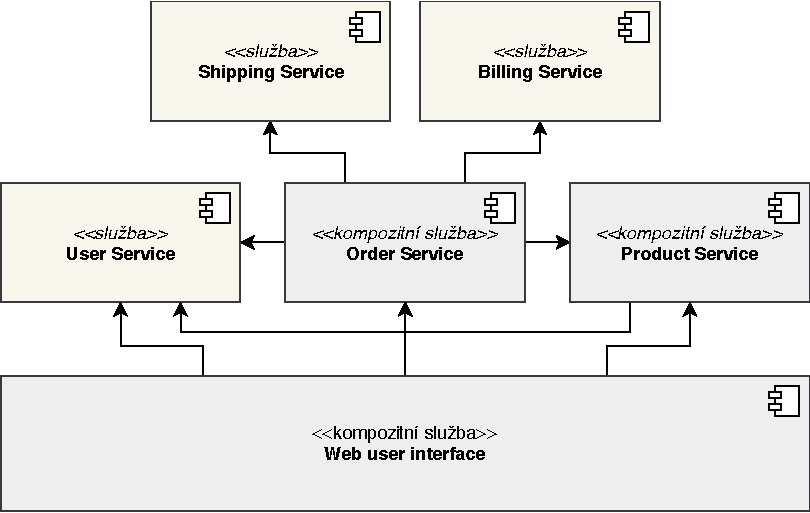
\includegraphics[keepaspectratio=true, width=0.8\linewidth]{figures/example-system.pdf}
    \caption{Komponenty ukázkového e-commerce systému}
    \label{fig:example-system}
\end{figure}

\paragraph{Billing service}

Služba \textit{Billing service} má na starosti funkcionalitu t\'ykaj\'{\i}c\'{\i} se fakturace objednávek
a byla implementována v jazyce Java s použit\'{\i}m frameworku Spring Boot\footnote{\url{https://projects.spring.io/spring-boot/}}.

\paragraph{Order service}

Kompozitn\'{\i} služba \textit{Order service} slouž\'{\i}c\'{\i} pro vytvářen\'{\i} a správu objednávek
byla implementována v jazyce Java a jej\'{\i} \gls{API} bylo sestaveno za použit\'{\i} frameworku Spring
Boot, jak je ukázáno ve zdrojovém kódu~\ref{lst:order-service-springboot}, kde
je ukázka obsluhy požadavků na v\'ypis zbož\'{\i} v koš\'{\i}ku uživatele.

\lstinputlisting[
caption={Ukázka využit\'{\i} frameworku Spring Boot pro účely Order service},
label={lst:order-service-springboot},
language=Java,
%frame=single,
]
{code/order_service.java}

\paragraph{Product service}

Služba \textit{Product service} realizuje \gls{UC} t\'ykaj\'{\i}c\'{\i} se
prohl\'{\i}žen\'{\i} a administrac\'{\i} nab\'{\i}zen\'ych
produktů a jejich skladov\'ych zásob. Služba byla implementována v jazyce Python.
Pro vytvořen\'{\i} \gls{REST} \gls{API} služby byl využit
light-weight framework \textit{Flask}\footnote{\url{http://flask.pocoo.org/}}.
Ve zdrojovém kódu~\ref{lst:product-service-flask} je znázorněno použit\'{\i}
tohoto frameworku pro obsluhu požadavku na v\'ypis všech produktů.

\lstinputlisting[
caption={Ukázka využit\'{\i} frameworku Flask pro účely Product service},
label={lst:product-service-flask},
language=Python,
%frame=single,
]
{code/product_service.py}

\paragraph{Shipping service}

Služba \textit{Shipping service} má na starosti funkcionalitu t\'ykaj\'{\i}c\'{\i} se odes\'{\i}lán\'{\i} objednávek
a byla implementována v jazyce Java s použit\'{\i}m frameworku Spring Boot.

\paragraph{User service}

Služba \textit{User service} realizuj\'{\i}c\'{\i} funkcionalitu t\'ykaj\'{\i}c\'{\i} se uživatelsk\'ych účtů byla
implementována v jazyce JavaScript na platformě Node.js s použit\'{\i}m
frameworku Express\footnote{\url{https://expressjs.com/}}. Ve zdrojovém kódu~\ref{lst:user-service-expressjs}
je ukázka mapován\'{\i} controllerů na \gls{URL} \code{/users} a různé metody protokolu \gls{HTTP}.

\lstinputlisting[
caption={Ukázka využit\'{\i} frameworku Express.js pro účely User service},
label={lst:user-service-expressjs},
language=JavaScript,
%frame=single,
]
{code/user_service.js}

\paragraph{Webové uživatelské rozhran\'{\i}}

Služba, která slouž\'{\i} uživatelům ukázkového systému jako webové uživatelské
rozhran\'{\i}, byla implementována v jazyce Java s použit\'{\i}m frameworku Spring Boot.
Na sn\'{\i}mku~\ref{fig:example-screenshot} je vidět UI ukázkového systému,
konkrétně informován\'{\i} uživatele o tom, že se nepodařilo přidat produkt
do koš\'{\i}ku, protože bylo porušeno byznysové pravidlo – koš\'{\i}k nesm\'{\i} obsahovat
v\'{\i}ce než 10 položek.

\paragraph{Centráln\'{\i} správa byznysov\'ych pravidel}

Do ukázkového systému byl nasazen také systém pro centráln\'{\i} správu byznysov\'ych kontextů,
kter\'y je popsan\'y v sekci~\ref{sec:central-administration}. Systém byl napojen na všechny
služby systému, kromě webového \gls{UI}, a bylo úspěšně demonstrováno, že lze za běhu systému
dynamicky upravovat byznysové kontexty, resp. jejich byznysová pravidla.

\paragraph{Běhové prostřed\'{\i} služeb}
Pro jednoduché spuštěn\'{\i} celého ukázkového systému byla využita technologie
Docker~\cite{merkel2014docker}, která umožňuje vytvořit virtuáln\'{\i} běhové prostřed\'{\i}
pro aplikaci pomoc\'{\i} kontejnerizace využ\'{\i}vaj\'{\i}c\'{\i} virtualizaci nad operačn\'{\i}m systémem.
Uživatel si nadefinuje tzv. \textit{image}, kter\'y se skládá z jednotliv\'ych vrstev.
Základn\'{\i} vrstvou je operačn\'{\i} systém, dalš\'{\i}mi mohou b\'yt jednotlivé knihovny instalované do systému.
Př\'{\i}klad definice image pomoc\'{\i} technologie Docker je znázorněn ve zdrojovém
kódu~\ref{lst:docker-image}. Konkrétně se jedná o definici image, kter\'y
rozšiřuje oficiáln\'{\i} image \code{library/node:9.11.1}\footnote{\url{https://hub.docker.com/\_/node/}}
stavěj\'{\i}c\'{\i} nad operačn\'{\i}m systémem \textit{Linux}\footnote{\url{https://www.linuxfoundation.org/projects/linux/}},
a přidává vrstvy s prototypem knihovny pro platformu Node.js.

\lstinputlisting[
caption={Ukázka zápisu Docker image obsahuj\'{\i}c\'{\i} knihovnu pro platformu Node.js},
label={lst:docker-image},
language=Dockerfile,
%frame=single,
]
{code/dockerfile_nodejs.txt}

\paragraph{Spouštěn\'{\i} služeb}
Pro samotné spuštěn\'{\i} byla využita funkce \textit{Compose}, která umožňuje
definovat a spouštět v\'{\i}ce-kontejnerové aplikace. Ve zdrojovém kódu~\ref{lst:docker-compose}
můžeme vidět zápis Order service. Pro jej\'{\i} image je použit \code{filipklimes-diploma/example-order-service}.
V sekci \code{ports} deklarujeme, že služba má m\'{\i}t z vnějšku př\'{\i}stupn\'y port \code{5501}, na kterém poskytuje své
\gls{REST} \gls{API}, a port \code{5551}, nak terém poskytuje své gRPC \gls{API} pro sd\'{\i}lené byznysov\'ych kontextů. Order service je závislá
na Product, Billing, Shipping a User service, což explicitně specifikujeme v sekci \code{depends\_on},
aby Docker Compose mohl spustit služby ve správném pořad\'{\i}. Nakonec pomoc\'{\i} \code{links} deklarujeme,
že pro kontejner, ve kterém Order Service poběž\'{\i}, maj\'{\i} b\'yt na s\'{\i}ti př\'{\i}stupné služby \code{product}, \code{user},
\code{billing} a \code{shipping}. Vše je popsáno ve formátu \gls{YAML}, kter\'y je vhodný
pro konfiguračn\'{\i} soubory díky jeho snadné čitelnosti pro člověka a jednoduchému použ\'{\i}ván\'{\i}.

\lstinputlisting[
caption={Ukázka zápisu v\'{\i}ce-kontejnerové aplikace pro Docker Compose},
label={lst:docker-compose},
language=Yaml,
%frame=single,
]
{code/docker_compose.yml}

\section{Srovnán\'{\i} s konvenčn\'{\i}m př\'{\i}stupem}

%\goal{Ukázka na konkrétn\'{\i}m př\'{\i}kladě}
Z tabulky~\ref{tbl:business-contexts} plyne, že 55 \% byznysov\'ych pravidel v ukázkovém systému je
využ\'{\i}váno ve v\'{\i}ce kontextech, a polovina je využ\'{\i}vána např\'{\i}č v\'{\i}ce službami.
V tabulce~\ref{tbl:duplication} je přehledně shrnuto, která pravidla jsou využ\'{\i}vána ve kter\'ych službách.
Při použit\'{\i} konvenčn\'{\i}ho př\'{\i}stupu by tato pravidla bylo nutné implementovat alespoň
jednou pro každou ze služeb, za předpokladu, že by nedocházelo k duplikac\'{\i}m ve službách samotn\'ych.
Manuáln\'{\i} duplikace nav\'{\i}c přináš\'{\i} nutnost synchronizovat podobu pravidla při každém změnovém
ř\'{\i}zen\'{\i}, což zvyšuje náklady na v\'yvoj a riziko lidské chyby.

\begin{table}
    \centering
    \begin{tabularx}{\textwidth}{ l X | l X }
        \hline
        \textbf{\#} & \textbf{Použito ve službách} & \textbf{\#} & \textbf{Použito ve službách} \\ \hline \hline
        \textbf{BR01} & user & \textbf{BR11} & auth, order, product \\
        \textbf{BR02} & order, product & \textbf{BR12} & product \\
        \textbf{BR03} & order, product & \textbf{BR13} & product \\
        \textbf{BR04} & order, shipping & \textbf{BR14} & product \\
        \textbf{BR05} & billing, order & \textbf{BR15} & order \\
        \textbf{BR06} & order, user & \textbf{BR16} & (auth), product, user \\
        \textbf{BR07} & order & \textbf{BR17} & product \\
        \textbf{BR08} & order & \textbf{BR18} & user \\
        \textbf{BR09} & order, shipping & \textbf{BR19} & user \\
        \textbf{BR10} & (auth), order, product & \\
        \hline
    \end{tabularx}
    \caption{Využit\'{\i} byznysov\'ych pravidel ve službách ukázkového systému}
    \label{tbl:duplication}
\end{table}

%\goal{V\'yhody frameworku}
D\'{\i}ky použit\'{\i} navrženého frameworku je však možné každé pravidlo nadefinovat centrálně
a framework se postará o jeho automatickou integraci do všech částí systému, kde má být aplikováno.
D\'{\i}ky tomu je možno byznysová pravidla, resp. kontexty, spravovat pomoc\'{\i} nástroje pro
centráln\'{\i} správu, kter\'y je součást\'{\i} navrženého frameworku. Z toho vypl\'yvá
sn\'{\i}žen\'{\i} nároků na v\'yvoj a sn\'{\i}žené riziko lidské chyby.

%\goal{Nev\'yhody použit\'{\i}}
Jako nev\'yhodu použit\'{\i} frameworku lze považovat počátečn\'{\i} investici v
podobě integrace knihoven do služeb systému. Zvážit mus\'{\i}me i cenu popisu byznysov\'ych pravidel
v \gls{DSL}, kter\'y se musej\'{\i} v\'yvojáři systému naučit nav\'{\i}c oproti programovac\'{\i}mu jazyku,
ve kterém popisuj\'{\i} služby. Dále je při návrhu systému potřeba identifikovat byznysové kontexty, jejich
hirearchii a vzájemnou vazbu s byznysov\'ymi pravidly, aby bylo možno framework efektivně využ\'{\i}vat.
To může vyžadovat v\'{\i}ce času, než klasick\'y návrh.

%\goal{Závěr}
Navržen\'y framework tedy oproti konvenčn\'{\i}mu př\'{\i}stupu nab\'{\i}z\'{\i} možnost z\'{\i}skat dlouhodobě
nižš\'{\i} náklady na v\'yvoj za cenu počátečn\'{\i} investice. Architekt softwarového systému mus\'{\i} př\'{\i}padné nasazen\'{\i}
frameworku zvážit z několika úhlů pohledu a posoudit, zda bude životnost systému dostatečně dlouhá a systém
dostatečně velk\'y. Dalš\'{\i}m podstatn\'ym bodem ke zvážen\'{\i} je reálná m\'{\i}ra znovupoužit\'{\i} byznysov\'ych pravidel.
Mohou existovat domény, ve kter\'ych bude nasazen\'{\i} frameworku jistě mnohem vhodnějš\'{\i}, než v jin\'ych.
D\'{\i}ky provedené př\'{\i}padové studii bylo prokázáno, že v \gls{SOA} lze efektivně řešit sdílení byznysov\'ych pravidel
navržen\'ym způsobem.

\section{Shrnut\'{\i}}

Tato kapitola popisuje, jak\'ym způsobem byly testovány prototypy knihoven
pro platformy jazyků Java a Python a pro platformu Node.js. T\'{\i}m byla otestována
jejich správná fukcionalita. Dále kapitola specifikuje ukázkový systém, na kterém byla
provedena demonstrace použit\'{\i} frameworku, a popisuje jeho implementaci.
Tím bylo otestováno, že navržen\'y framework je funkčn\'{\i},
splňuje požadavky identifikované v sekci~\ref{sec:implementation-requirements}
a prokazuje reálné snížení manuální duplikace byznysových pravidel oproti
konvenčn\'{\i}mu př\'{\i}stupu k návrhu a implementaci softwarov\'ych systému.

%\usepackage[T1]{fontenc}
%\usepackage[utf8]{inputenc}

%!TEX ROOT=../diploma-thesis.tex

\chapter{Závěr}\label{ch:zaver}

\section{Anal\'yza dopadu použit\'{\i} frameworku}

\section{Budouc\'{\i} rozšiřitelnost frameworku}

\subsection{Kvalitní doménově specifický jazyk}
Zadáním této práce nebylo zkonstruovat vlastní \gls{DSL}
k účelům automatické distribuce a centrální správy byznys pravidel,
nicméně v sekci~\ref{sec:implementation-requirements} jsme potřebu takového
jazyka jasně identifikovali a následně v kapitole~\ref{ch:reserse}
jsme došli k závěru, že momentálně neexistuje vhodné \gls{DSL},
které by splňovalo všechny naše požadavky a mohli bychom ho
využít pro naše účely. V rámci implementace prototypu knihoven
jsme navrhli a implementovali vlastní \gls{DSL} v jazyce \gls{XML},
jak jsme popsali v sekci~\ref{sec:dsl-impl}. Tento jazyk je však
velmi omezený a snaží se vyhovět co nejnižším nárokům na implementaci.
Sestavení kvalitního jazyka pro naše účely je tématem nejméně pro
bakalářskou práci. Nicméně, námi navržený framework je schopen toto
rozšíření pojmout, stačí doimplementovat plug-in, který se bude starat
o převod z daného \gls{DSL} do paměťové reprezentace byznysového kontextu.

Kvalitní jazyk by měl kromě výše zmíněných požadavků pro zachycení
pravidla poskytovat co nejpřehlednější zápis, aby ho mohl snadno číst a zapisovat
nejen vývojář, ale i doménový expert či administrátor systému. Tím by se
ještě zvýšil přínos centrální administrace byznysových pravidel, kterou jsme v rámci
této práce implementovali a popsali v sekci~\ref{sec:central-administration}.
Můžeme také diskutovat, že by jazyk pro popis byznysových kontextů sloužil pouze
jako platforma a samotná pravidla by byla popsána v \gls{DSL} vytvořeném na míru
byznysové doméně, pro kterou by byl implementován systém využívající našeho frameworku.

\subsection{Integrace frameworku s uživatelským rozhraním}

V sekci~\ref{sec:architecture} jsme nastínili způsob, jakým lze využívat náš framework.
Jedním ze způsobů je integrace do uživatelského rozhraní. Autoři přístupu \gls{ADDA} již
vyvinuli způsob, kterým lze integrovat vyhodnocování
byznysových pravidel v uživatelském rozhraní~\cite{cemus2017separation}. Propojení s
naším frameworkem by znamenalo pouze implementovat adaptér, který by převáděl námi
použitou reprezentaci byznysového pravidla do podoby, kterou je schopen využívat
aspect weaver v \gls{UI}. Tím by se rozšířila působnost našeho frameworku a zároveň
by se zvýšil uživatelský komfort \gls{EIS}, který framework využívá, díky real-time
validaci vstupních hodnot formulářů.

\subsection{Integrace frameworku s datovou vrstvou}

Jak jsme také zmínili v sekci~\ref{sec:architecture}, integrace do datové vrstvy
je také jednou z možností. Podobně jako v případě \gls{UI}, autoři přístupu
\gls{ADDA} navrhují způsob, kterým lze automaticky distribuovat post-conditions
do datové vrstvy transformováním jejich podmínek do výrazů v \gls{SQL}
jazyce~\ref{cemus2015automated}. Aplikováním příslušného aspect weaveru by byl
zvýšen dosah frameworku a byla by pokryta další oblast, ve které může docházet
k manuální duplikaci byznysových pravidel.

\section{Možnost\'{\i} uplatněn\'{\i} navrženého frameworku}

\section{Dalš\'{\i} možnosti uplatněn\'{\i} \gls{AOP} v \gls{SOA}}

\todo{
\begin{itemize}
    \item{Extrakce dokumentace}
    \item{Extrakce byznysového modelu}
    \item{Konfigurace prostřed\'{\i}}
\end{itemize}
}

\section{Shrnut\'{\i}}

\todo{
\begin{itemize}
    \item{Dosáhli jsme c\'{\i}lů práce}
    \item{Stručné shrnut\'{\i} co všechno a jak jsme udělali}
\end{itemize}
}


\bibliographystyle{csplainnat}

%bibliographystyle{plain}
%\bibliographystyle{psc}
{
%JZ: 11.12.2008 Kdo chce mit v techto ukazkovych odkazech take odkaz na CSTeX:
\def\CS{$\cal C\kern-0.1667em\lower.5ex\hbox{$\cal S$}\kern-0.075em $}
\bibliography{reference}
}

\appendix

%!TEX ROOT=../diploma-thesis.tex

\renewcommand*{\glsnamefont}[1]{\textbf{#1}}
\setlength{\glsdescwidth}{0.7\textwidth}
\printglossary[type=\acronymtype,title={Seznam použit\'ych zkratek}]\label{ch:shortcuts}

%!TEX ROOT=../diploma-thesis.tex

\chapter{Přehledové obrázky a sn\'{\i}mky}

\vspace{4\baselineskip}

\begin{figure}[h]
    \centering
    \fbox{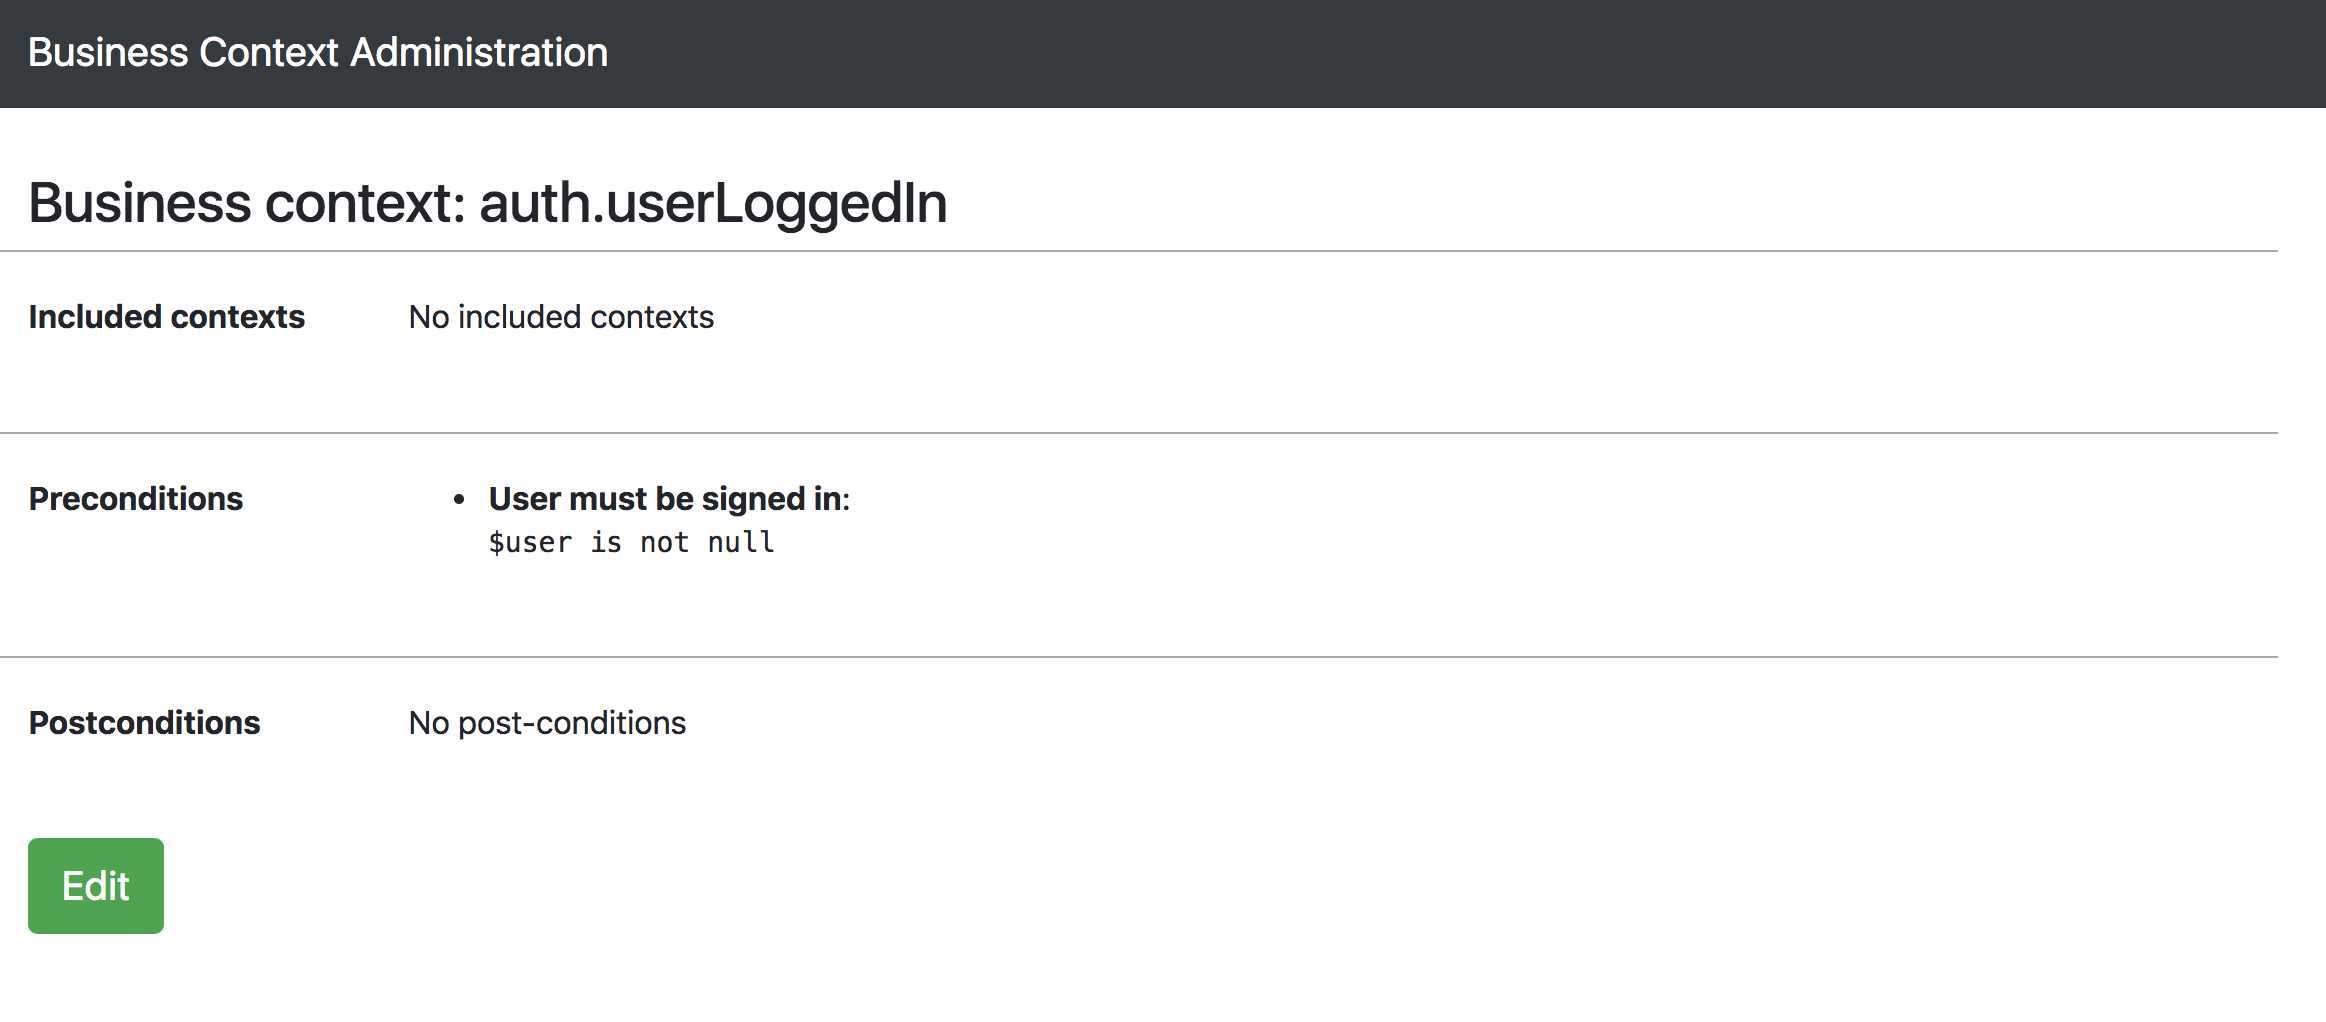
\includegraphics[width=0.9\linewidth]{figures/business-context-detail.png}}
    \caption{Detail byznysového kontextu v centráln\'{\i} administraci}
    \label{fig:screenshot-context-detail}
\end{figure}

\begin{figure}
    \centering
    \fbox{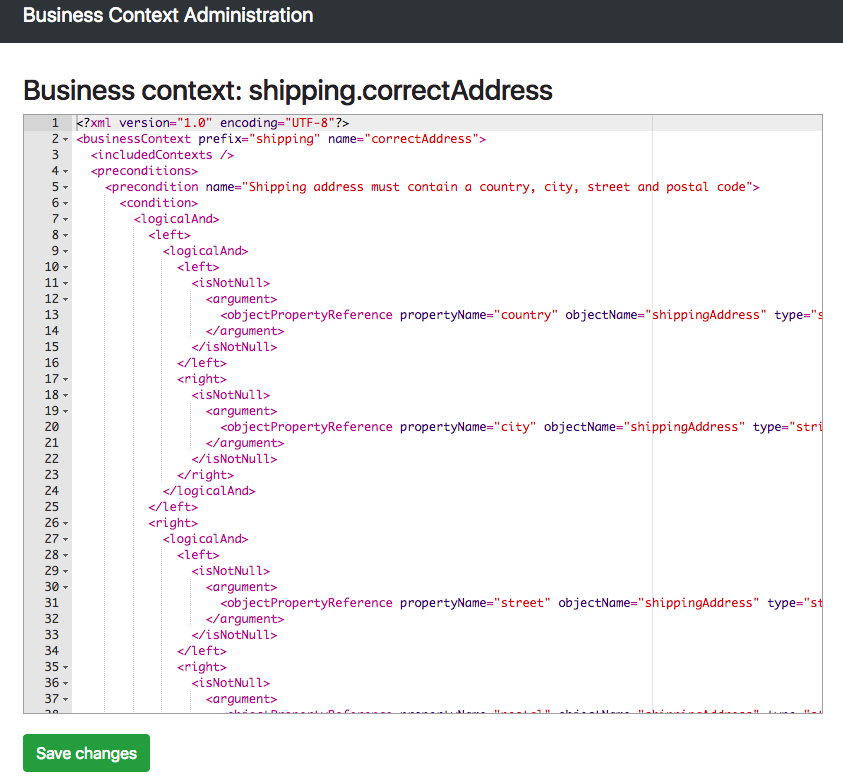
\includegraphics[width=0.7\linewidth]{figures/business-context-edit.png}}
    \caption{Formulář pro vytvořen\'{\i} nebo úpravu byznysového kontextu v centráln\'{\i} administraci}
    \label{fig:screenshot-context-edit}
\end{figure}

\begin{figure}
    \centering
    \fbox{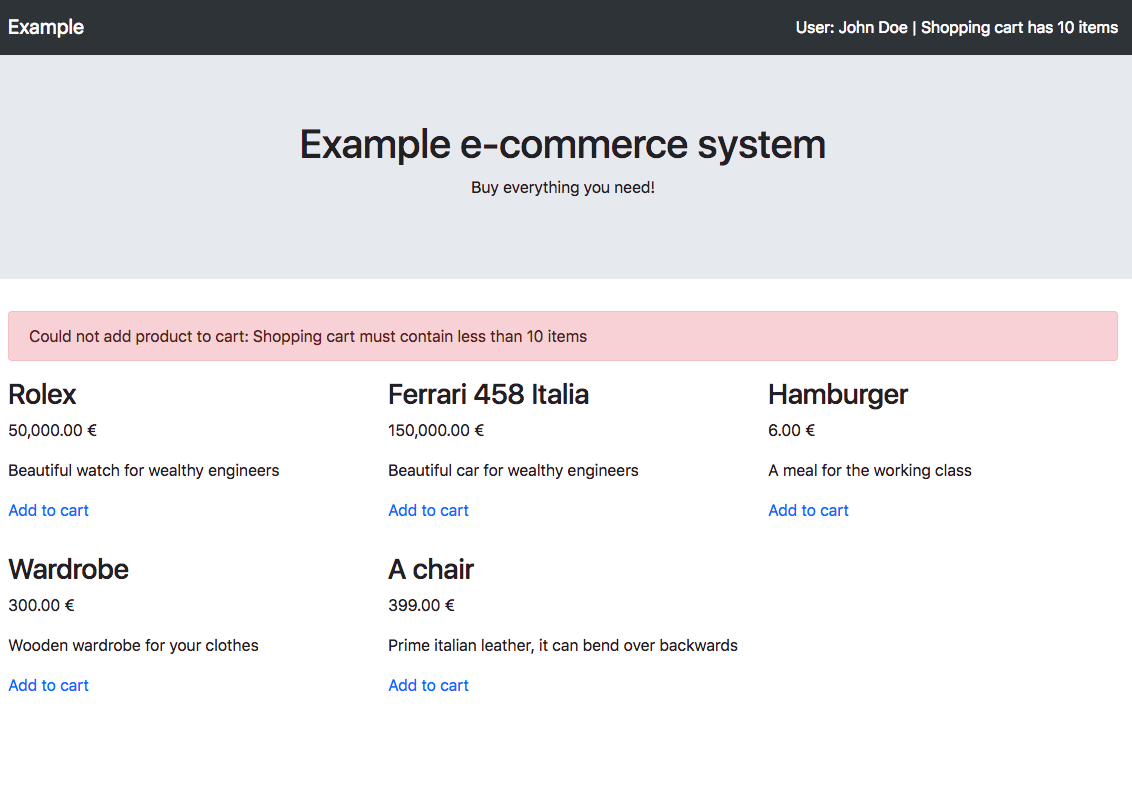
\includegraphics[width=0.7\linewidth]{figures/add-product-to-cart-fail.png}}
    \caption{Propagace byznysového pravidla při přidáván\'{\i} produktu do koš\'{\i}ku v ukázkovém systému}
    \label{fig:example-screenshot}
\end{figure}


\begin{sidewaysfigure}[ht]
    \centering
    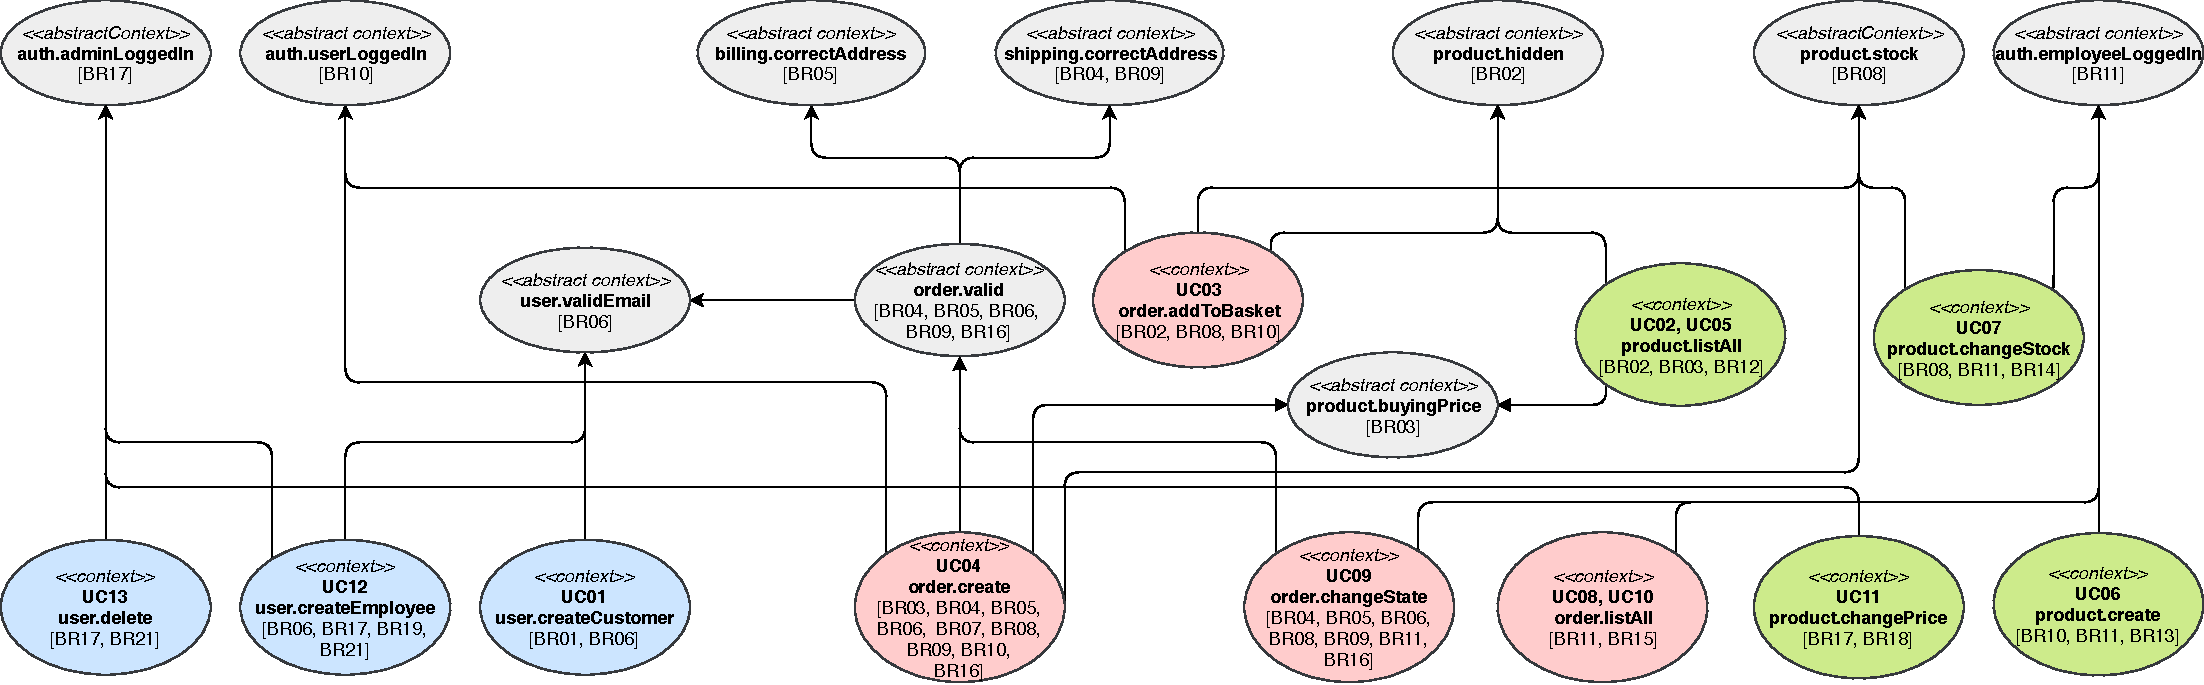
\includegraphics[keepaspectratio=true, width=\linewidth]{figures/example-system-context-hierarchy.pdf}
    \caption{Diagram hirearchie byznysov\'ych kontextů ukázkového systému}
    \label{fig:example-system-context-hirearchy}
\end{sidewaysfigure}
%!TEX ROOT=../diploma-thesis.tex

\chapter{Obsah přiloženého CD}

\begin{Verbatim}[fontsize=\footnotesize]
    |-- central-administration/      Systém centrální administrace byz. kontextů
    |
    |-- example/                     Ukázkový e-commerce systém
    |  |-- billing/                  Fakturační služba
    |  |-- order/                    Objednávková služba
    |  |-- product/                  Produktová služba
    |  |-- shipping/                 Doručovací služba
    |  |-- ui/                       Uživatelské rozhraní
    |  |-- user/                     Uživatelská služba
    |
    |-- java/                        Prototyp knihovny pro jazyk Java
    |  |-- business-context/         Jádro knihovny
    |  |-- business-context-aspectj/ Adaptér pro framework AspectJ
    |  |-- business-context-grpc/    Knihovna pro síťovou komunikaci využívající gRPC
    |  |-- business-context-xml/     Knihovna pro načítání a zápis byz. kontextů do XML
    |
    |-- nodejs/                      Prototyp knihovny pro platformu Node.js
    |  |-- business-context/         Jádro knihovny
    |  |-- business-context-grpc/    Knihovna pro síťovou komunikaci využívající gRPC
    |  |-- business-context-xml/     Knihovna pro načítání a zápis byz. kontextů do XML
    |
    |-- proto/                       Schéma síťové komunikace ve formátu Proto Buffers
    |
    |-- python/                      Prototyp knihovny pro jazyk Python
    |  |-- business_context/         Jádro knihovny
    |  |-- business_context_grpc/    Knihovna pro síťovou komunikaci využívající gRPC
    |  |-- business_context_xml/     Knihovna pro načítání a zápis byz. kontextů do XML
    |
    |-- xml/                         Schéma XML pro zápis byz. kontextů
    |
    |-- text/                        Zdrojový kód bakalářské práce v jazyce LaTeX
\end{Verbatim}


\end{document}
